\documentclass[sigconf,screen]{acmart}

% KDD 2028 (dates and venue TBA)
\copyrightyear{2028}
\acmYear{2028}
\acmConference[KDD '28]{Proceedings of the 34th ACM SIGKDD Conference on Knowledge Discovery and Data Mining}{TBA, 2028}{TBA}
\acmBooktitle{Proceedings of the 34th ACM SIGKDD Conference on Knowledge Discovery and Data Mining (KDD '28), TBA, 2028, TBA}
\usepackage{hyperref}
\usepackage{mathtools}
\usepackage{enumitem}
\usepackage{pgfplots}
\pgfplotsset{compat=1.18}
\usepgfplotslibrary{groupplots}
\usetikzlibrary{patterns}


% \usepackage[letterpaper,margin=0.8in]{geometry}

\newlist{todolist}{itemize}{2}
\setlist[todolist]{label=$\square$}
\newcommand{\done}{\rlap{$\square$}{\raisebox{2pt}{\large\hspace{1pt}\checkmark}}\hspace{-2.5pt}}


\usepackage{listings}
\usepackage[dvipsnames]{xcolor}
\usepackage{colortbl}

\definecolor{codegreen}{rgb}{0,0.6,0}
\definecolor{codepurple}{rgb}{0.58,0,0.82}
\definecolor{backcolour}{rgb}{0.96,0.96,0.94}

\lstdefinestyle{cppstyle}{
  language=C++,
  basicstyle=\ttfamily\footnotesize,
  keywordstyle=\color{blue},
  commentstyle=\color{codegreen},
  stringstyle=\color{codepurple},
  backgroundcolor=\color{backcolour},
  frame=single,
  columns=fullflexible,
  breaklines=true,
  showstringspaces=false,
  xleftmargin=1em,
  aboveskip=0.5em, belowskip=0.5em,
}
\lstset{style=cppstyle}

\newcommand{\TODO}[1]{\textbf{\textcolor{red}{#1}}}
\newcommand{\Claude}[1]{\textbf{\textcolor{YellowOrange}{#1}}}

% Inconsolata has no italic: substitute upright silently (no font warnings).
{\fontencoding{T1}\fontfamily{zi4}\selectfont}{\fontencoding{TS1}\fontfamily{zi4}\selectfont}
\DeclareFontShape{T1}{zi4}{m}{it}{<->ssub*zi4/m/n}{}
\DeclareFontShape{TS1}{zi4}{m}{it}{<->ssub*zi4/m/n}{}

\title{Distributed Training of Gradient-Boosted Trees with Sparse Oblique Splits}
\author{Ariel Lubonja}
\email{ariel@cs.jhu.edu}
\affiliation{
  \institution{Johns Hopkins University}
  \city{Baltimore}
  \state{Maryland}
  \country{USA}
}

\author{Jungsang Yoon}
\email{jyoon72@jh.edu}
\affiliation{
  \institution{Johns Hopkins University}
  \city{Baltimore}
  \state{Maryland}
  \country{USA}
}

\author{Haoyin Xu}
\email{hx@jhu.edu}
\affiliation{
  \institution{Johns Hopkins University}
  \city{Baltimore}
  \state{Maryland}
  \country{USA}
}

\author{Richard Stotz}
\email{richardstotz@google.com}
\affiliation{
  \institution{Google}
  \city{Zurich}
  \country{Switzerland}
}

\author{Jeffrey Hetherly}
\email{hetherly@google.com}
\affiliation{
  \institution{Google}
  \city{San Francisco}
  \state{California}
  \country{USA}
}

\author{Mathieu Guillame-Bert}
\email{gbm@google.com}
\affiliation{
  \institution{Google}
  \city{Zurich}
  \country{Switzerland}
}

\author{Vladimir Braverman}
\email{vova@cs.jhu.edu}
\affiliation{
  \institution{Johns Hopkins University}
  \city{Baltimore}
  \state{Maryland}
  \country{USA}
}

\author{Joshua T. Vogelstein}
\email{jovo@jhu.edu}
\affiliation{
  \institution{Johns Hopkins University}
  \city{Baltimore}
  \state{Maryland}
  \country{USA}
}

\author{Randal Burns}
\email{randal@cs.jhu.edu}
\affiliation{
  \institution{Johns Hopkins University}
  \city{Baltimore}
  \state{Maryland}
  \country{USA}
}

\renewcommand{\shortauthors}{Lubonja et al.}

\makeatletter
% Full-width \twocolumn[] blocks act as floats: lift acmart's \vspace warning like figure* does.
\newcommand{\floatblock}{\let\@vspace\@vspace@orig\let\@vspacer\@vspacer@orig}
\makeatother

\begin{document}

\ccsdesc[500]{Computing methodologies~Classification and regression trees}
\ccsdesc[300]{Computing methodologies~Distributed algorithms}
\keywords{gradient boosted trees, sparse oblique splits, distributed training}

\maketitle

\section{Work log - Weekly TODOs}

\textit{Ariel TODOs by Nov-10}

\textbf{\textit{Accuracy cost of parititioning columns: }}

\TODO{ensure we're measuring on datasets where SPO > AA accuracy}

\textcolor{cyan}{\done~2. Fix single vs. Distributed full replication accuracy + cross-column comms.} Fig.~\ref{fig:column-replication-ydf}, Sec.~\ref{sec:cross-network-projections}

Tradeoff of Extra memory vs. Accuracy: policy × amount (e.g. 120 \% storage) vs accuracy. \textbf{4 plots}: $0\% \to 100\%$ replication, under column assignment method. \textbf{100\% replication is equivalent to local SPO}
    \begin{todolist}
        \item[\textcolor{gray}{\done}] \textcolor{gray}{Round-robin}. Fig.~\ref{fig:column-replication-ydf}
        \item Random
        \item if AA acc = SPO acc, any partition strategy should get similar accuracy. Start with datasets where SPO is better (perhaps trunk)
        \item Important columns in model trained on 1\% of the dataset
        \item Correlation-based: all pairs uplift graph. Together or apart?
        \item Jovo methods: Feature information, mini-patches
        \item[\textcolor{gray}{\done}] \textcolor{gray}{Do selected columns remain constant along trees?} See Fig.~\ref{fig:cc18-tree-feature-hist}
    \end{todolist}

\textbf{\textit{Procedural}}

\begin{todolist}
    \item[\textcolor{cyan}{\done}] \textcolor{cyan}{\href{https://github.com/google/yggdrasil-decision-forests/commit/2fe3a7fae5a3e8646401cd98f5c0a2a9d5d81653}{Richard's new} AA + SPO scan.} Table~\ref{tab:dist-accuracy-ydf}
    \begin{todolist}
        \item[\textcolor{cyan}{\done}] \textcolor{cyan}{implement and vastly increase projections (to YDF defaults).}
        \item[\textcolor{cyan}{\done}] \textcolor{cyan}{AA, SPO (train\_oblique\_forest.cc default params) vs. SPO (YDF default params). Table~\ref{tab:dist-accuracy-ydf}}
        \item[\textcolor{cyan}{\done}] \textcolor{cyan}{Richard's AA+SPO. \textbf{Include?} Didn't see much accuracy diff. Table~\ref{tab:dist-accuracy-ydf}}
    \end{todolist}
    \item \Claude{why is SPO faster than AA despite Presort time excluded?} Opus-high then Fable-max to verify.
    \item[\textcolor{gray}{\done}] \textcolor{gray}{Plot Barrier results} See Fig.~\ref{fig:yt8m-barriers}
    \begin{todolist}
        \item[\textcolor{gray}{\done}] \textcolor{gray}{Naive SPO with cross-node communication}. See Sec. \ref{sec:cross-network-projections}
    \end{todolist}
    \stepcounter{enumi}\item[\textcolor{gray}{\done}] \textcolor{gray}{(in-worker oblique) Replace std::sort with Highway VQSort}
    \item[\textcolor{cyan}{\done}] \textcolor{cyan}{Multiple runs for Training and accuracy (seed)} 5 seeds: Table~\ref{tab:column-replication-ydf}, Table~\ref{tab:cross-network}
    \item[\textcolor{cyan}{\done}] \textcolor{cyan}{Related Work review. Fable: are there any previous work red flags that strongly challenge the novelty of this work? something a reviewer would point to and say "how is this different from that?" run a review with fable-max, then run a 2nd fable-max agent to verify the first, and iterate until both are happy} Sec.~\ref{sec:related-work}
\end{todolist}


\section{Introduction}

% The timely story writes itself — tabular foundation models (TabPFN etc.) don’t scale to large data, GBDTs still win there, and you’re pushing the frontier of the thing that wins at scale. Lead with that in papers and talks, not “trees are still relevant.”

% Being excellent at the unfashionable-but-used thing is a good position, but only if you stay literate in the fashionable thing — which is what the 20% buys you. 20% on tabular llm - to GBT dynamic

Distributed Tree training offers two main advantages: training on very large data ($>$100m examples+) that does not fit in a single machine's memory, and distributed hyperparameter tuning. 

To our knowledge, no distributed tree learner searches sparse oblique splits when no worker holds every feature, which is what this paper does. This severely limits Sparse Oblique methods to datasets that are limited to a single machine. AutoML frequently selects SPO-GBT as the best method.

YDF has support for distributed training GBTs~\cite{ydf,guillamebert2018exact}: the distribution is among the features, i.e. different workers handle different features. This allows us to train on very large (deep \& wide) datasets, because each worker just needs (roughly) enough memory to hold the label column and the feature column. 


Distributed training has 0 support for Sparse oblique splits; mainly because it's nontrivial to implement: Workers would need to store the pseudo-features, or store enough features to construct the pseudo-features efficiently, without moving features around too much. 
Column-partitioned learners~\cite{abuzaid2016yggdrasil,guillamebert2018exact,ydf} assign each feature to one worker, which also builds the split's bitmap. An oblique split reads features held by several workers, so no single owner exists. YDF has all the primitives and the GBT implementation ready.


\subsection{Current YDF Distributed GBT}

\textbf{Different workers handle different features}. This is very scalable, as each worker needs $\sim O(2N)$ memory.

YDF Distributed training requires:

\begin{itemize}
    \item Manager - a single machine that comms to the workers.
    \item Workers, communicating via IP. \texttt{Multi\_THREAD} or \texttt{GRPC}
    \item a Shared Directory - a computation cache \& checkpointing in case of worker(s) failure
    \item a Sharded dataset (path): csv, tfrecord, Apache Beam. Sharded by column. Usually 10 shards / worker.
\end{itemize}

 [Source: \href{https://ydf.readthedocs.io/en/latest/tutorial/distributed_training/#setup}{YDF Docs}]

 \begin{figure*}[t]
    \centering
    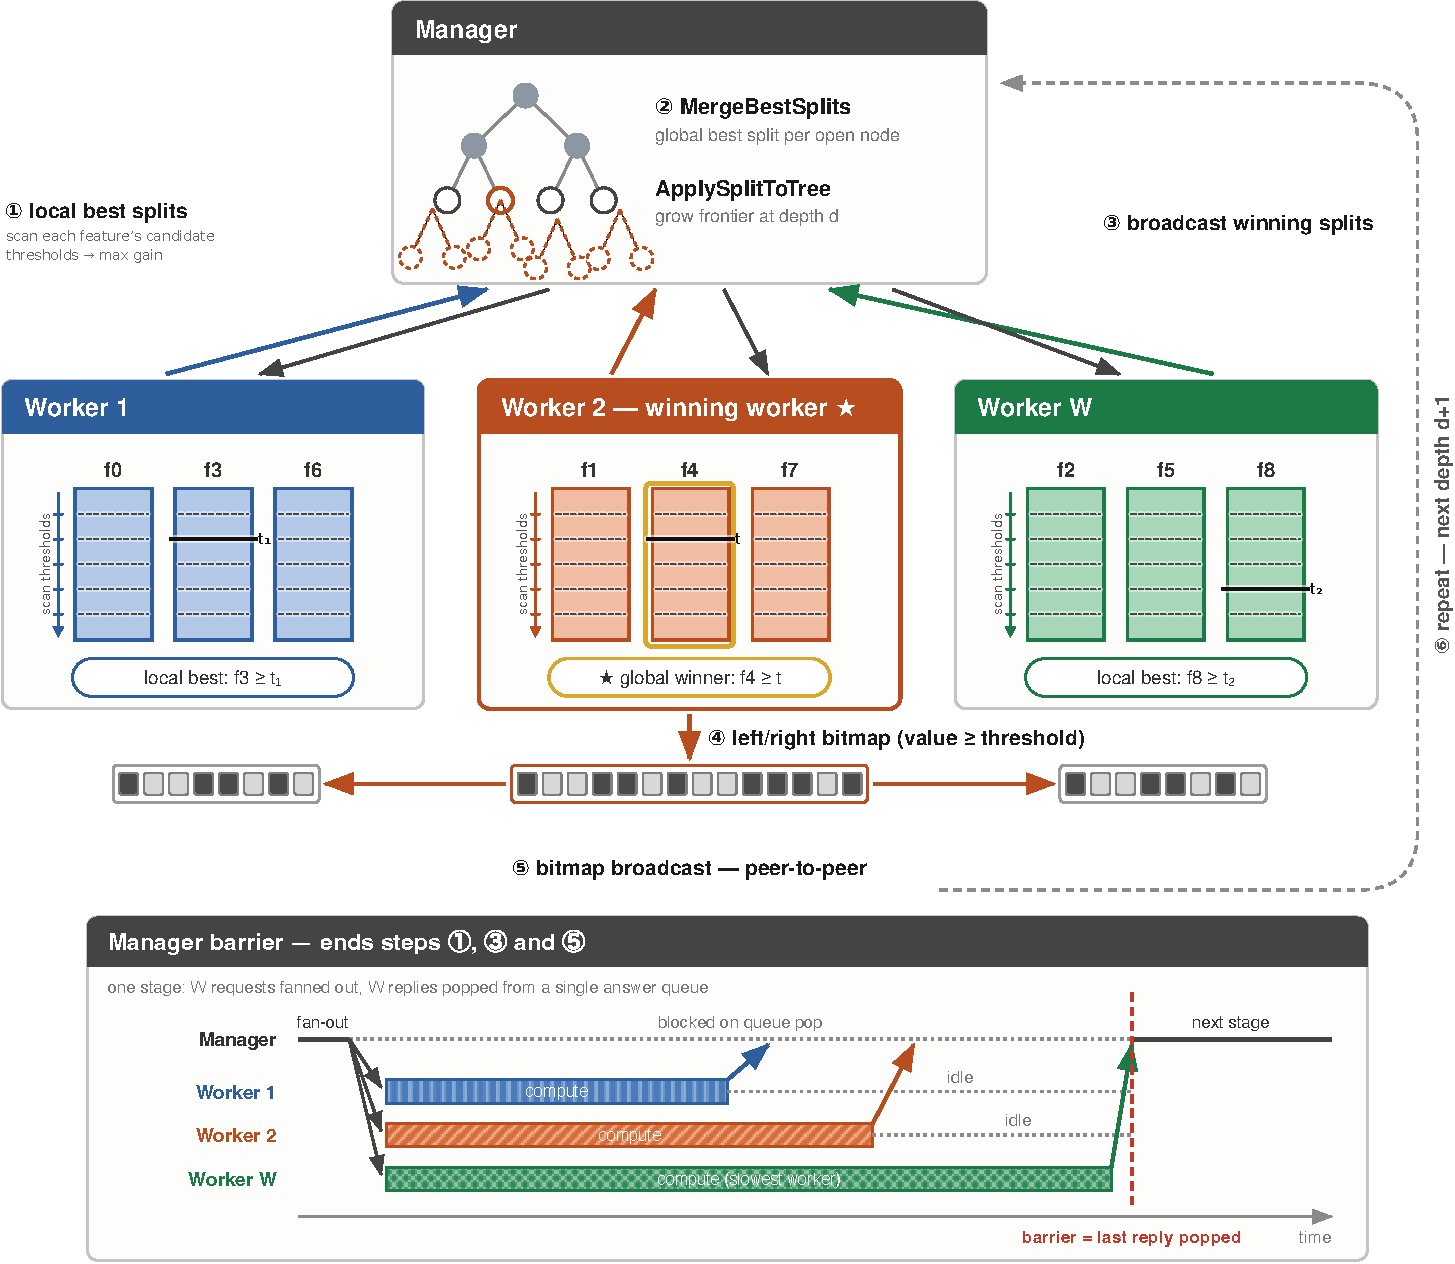
\includegraphics[width=.72\linewidth]{figures/method/distributed_gbt_training_loop_barrier.pdf}
    \caption{Distributed GBT Training Loop and manager barrier.}
    \Description{Manager-worker training loop with a barrier at each depth.}
    \label{fig:ydf-dist-gbt-training-loop}
\end{figure*}

\subsubsection{Load-balanced Data Sharding}

\begin{figure}[H]
    \centering
    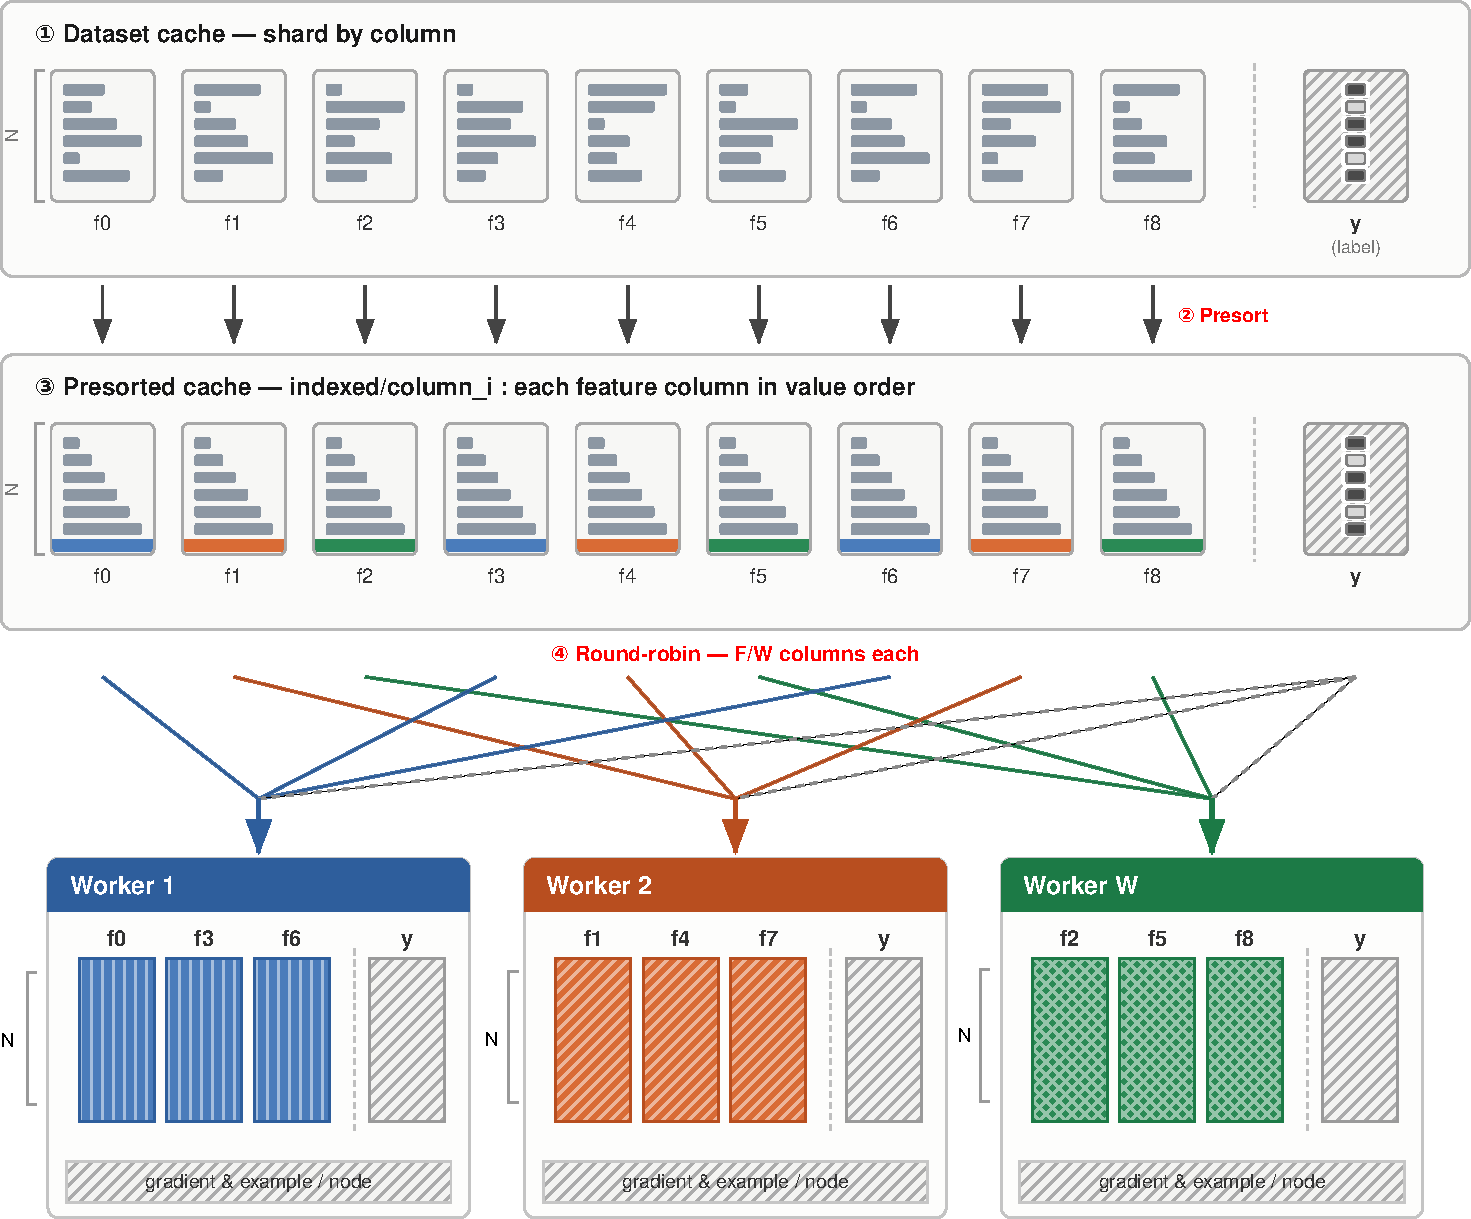
\includegraphics[width=1\linewidth]{figures/method/distributed_gbt_column_partitioning.pdf}
    \caption{Data Sharding illustration. Dataset is split by column, presorted, then round-robined in a load-balancing way.}
    \Description{Columns presorted and round-robined to workers.}
    \label{fig:ydf-dist-gbt-load-balancing}
\end{figure}

Feature columns are weighed by their expected compute expense : numerical features weigh $5.0$, Discretized weigh $1.0$ (\texttt{LoadBalancer::Initialize}). Numerical columns are Pre-Sorted (\texttt{dataset\_cache.cc::}\newline\texttt{SortNumericalColumns}).

\begin{enumerate}
    \item Shard dataset in shared directory, by column. 
        \begin{itemize}
            \item 1 column to 1 worker. No replication.
            \item \textbf{Main issue}: how to shard these once in SPO when they're sampled per node?
        \end{itemize}
    \item Presort Columns. \textbf{Not possible in SPO}
    \item Load-balanced column round-robin to workers, by compute intensity: 5 for Numeric, 1 for Discretized. \textbf{Issue 3. No fixed columns in SPO}
    \item Train
\end{enumerate}

\subsubsection{Training}

\paragraph{for depth in tree:}

\begin{enumerate}
    \item Workers scan their column subset, computing local \texttt{BestSplit} for nodes at a depth $d$ (in \texttt{FindBestSplitsWithThreadPool}). Local maxes are sent to Manager.
    \item Manager computes global Max in \texttt{MergeBestSplits}. Update manager's tree structure \texttt{ApplySplitToTree}.
    \item Manager broadcasts global winning split -\newline \texttt{EmitEvaluateSplits}
    \item Worker who owns Winning Column creates \textbf{bitmap} of examples to split into left-right. There is 1 winner per node at this depth
        \begin{lstlisting}
for (auto value : values) {
  const auto node_idx = example_to_node[example_idx];
  if (active_node_idx >= 0)
    active_node.writer.Write(value >= active_node.threshold);  // the bitmap
  example_idx++;
}
        \end{lstlisting}
    \item Winning workers broadcasts bitmap peer-to-peer
    \item Monitor workload for skew. Work-steal.
\end{enumerate}


\subsubsection{Approximate Splits}

AA-GBT offers approximate splits to further improve training speed. Very often, this can speed up training by 2x-5x without negative impact on quality. In our experiments, these are not used. Instead, the data is Presorted and Exact splits are run.

\section{Related Work}
\label{sec:related-work}

Oblique decision trees split on linear combinations of features rather than on a single feature. Breiman's original random forest paper proposed Forest-RC, which draws random linear combinations of a few inputs at each node~\cite{breiman}. OC1 searches for hyperplanes by hill climbing with random perturbations~\cite{murthy1994system}, canonical correlation forests derive the projection at each node from CCA~\cite{rainforth2015canonical}, and TAO learns sparse oblique trees by alternating optimization over the node hyperplanes~\cite{carreira2018alternating}, with bivariate trees as the two-feature special case~\cite{kairgeldin_bivariate_2024}. Sparse projection oblique random forests (SPO-RF)~\cite{tomita2020sparse} sample sparse random projections at each node and are implemented in treeple~\cite{treeple} and in YDF~\cite{ydf}, whose sparse oblique splits we optimize. SPO-RF is also the base learner of MIGHT, which trains forests to purity to obtain calibrated posteriors for biomedical screening~\cite{might1,might2}. Common to all of these methods is the fact that the feature being split exists only once the node's projection has been drawn and therefore cannot be presorted/pre-quantized before training.

Axis-aligned learners find splits either exactly or with histograms. Exact splitting sorts the candidate feature's values within the node or scans a pre-sorted index of the whole column: ranger~\cite{wright2017ranger}, XGBoost's exact method~\cite{chen2016xgboost} and YDF~\cite{ydf} pre-sort, and scikit-learn's forests sort in the node~\cite{pedregosa2011scikit}. Histogram splitting, the default in LightGBM~\cite{ke2017lightgbm}, CatBoost~\cite{prokhorenkova2018catboost}, XGBoost's histogram method~\cite{chen2016xgboost}, TF Boosted Trees~\cite{ponomareva2017tf} and Spark MLlib~\cite{meng2016mllib}, quantizes every feature once before training into a fixed number of bins, so that filling a node's histogram is a scatter-add over stored bin indices with no search in the loop. XGBoost's local proposal variant~\cite{chen2016xgboost} and YDF's histogram splits~\cite{ydf} instead recompute bin boundaries per node, from the node's quantiles, its value range, or at random. Further savings come from sharing work across nodes: histogram subtraction derives one child's histogram from the parent's~\cite{ke2017lightgbm}, CatBoost's oblivious trees split every node of a level on the same feature and bin grid~\cite{prokhorenkova2018catboost}, and GPU trainers assemble partial histograms per thread block~\cite{wenthundergbm19,xu2025scalagbm}. 

\textit{The partitioning landscape}

\begin{itemize}
    \item PLANET (Panda et al., VLDB 2009). Row-partitioned MapReduce tree ensembles with a central controller; the lineage of every data-parallel learner. Binned splits because exact ones would need a distributed sort per attribute.
    \item Fu, Jiang, Shao, Cui, “An Experimental Evaluation of Large Scale GBDT Systems” / Vero (VLDB 2019). Defines the row/column × row-store/column-store quadrants and derives the cost formulas. Shows vertical partitioning wins at high dimension and deep trees; places LightGBM feature-parallel as replicated.
    \item LightGBM (Ke et al., NIPS 2017) + its distributed guide. Data, feature and voting parallel modes; feature parallel keeps the full dataset on every worker, which is exactly why it dodges your problem.
    \item PV-Tree (Meng et al., NIPS 2016). Two-phase voting to cut data-parallel histogram traffic. Quantifies attribute-parallel placement cost as proportional to \#samples (your bitmap term).
    \item DimBoost (Jiang, Cui, Zhang, Fu, SIGMOD 2018). High-dimensional GBDT on parameter servers, row-partitioned. Closed access; cite via Vero.
    \item Also, unread this session: Ye et al., “Stochastic gradient boosted distributed decision trees” (CIKM 2009; horizontal vs vertical GBDT, Yggdrasil cites it as the vertical precedent); Vasiloudis et al., “Block-distributed GBT” (SIGIR 2019; 2-D row×column blocks, the hybrid quadrant you lack); Svore \& Burges (2011; full copy per worker, search split by feature).
\end{itemize}
% Added 2026-10-26 from the related-work check (ariel_notes/related_work/2026-10-26_distributed_spo/).
% Entries without a locator there (1-5, 7-10, 12-15) are from memory, not read in that pass: verify before final.

\textit{Classic parallel decision-tree induction}

\begin{itemize}
    \item \textit{Parallel Formulations of Decision-Tree Classification Algorithms} (Srivastava, Han, Kumar, Singh; Data Mining and Knowledge Discovery 1999). The canonical taxonomy of parallel tree construction: synchronous (data-parallel), partitioned (task-parallel per subtree) and hybrid. Our column-partitioned protocol is the synchronous, attribute-distributed case in this vocabulary.
    \item \textit{SPRINT: A Scalable Parallel Classifier for Data Mining} (Shafer, Agrawal, Mehta; VLDB 1996) and \textit{SLIQ: A Fast Scalable Classifier for Data Mining} (Mehta, Agrawal, Rissanen; EDBT 1996). Presorted attribute lists split across processors; splitting a node requires exchanging record ids proportional to $N$. The origin of the per-level placement cost our bitmap broadcast pays, and of the obstacle for splits that read several attributes.
    \item \textit{ScalParC: A New Scalable and Efficient Parallel Classification Algorithm for Mining Large Datasets} (Joshi, Karypis, Kumar; IPPS 1998). Removes SPRINT's $O(N)$ per-processor memory with a distributed hash table; shows that placement bookkeeping, not split finding, bounds attribute-distributed designs.
    \item \textit{Communication and Memory Efficient Parallel Decision Tree Construction} (Jin, Agrawal; SDM 2003). Data-parallel construction that prunes candidate splits statistically to cut communication; an early communication-versus-exactness trade-off of the kind our cross-worker options face.
    \item \textit{A Streaming Parallel Decision Tree Algorithm} (Ben-Haim, Tom-Tov; JMLR 2010). Data-parallel training with mergeable histograms, the basis of the histogram-allreduce family. There a projection is local to every worker, so oblique splits cost no extra communication but lose exact thresholds.
\end{itemize}

\textit{Distributed GBDT designs}

\begin{itemize}
    \item \textit{Stochastic Gradient Boosted Distributed Decision Trees} (Ye, Chow, Chen, Zheng; CIKM 2009). The first GBDT study of horizontal (MapReduce) against vertical (MPI) partitioning, finding the vertical version faster; the earliest precedent for feature-partitioned boosting.
    \item \textit{Large-Scale Learning to Rank Using Boosted Decision Trees} (Svore, Burges; in Scaling Up Machine Learning, 2011). Every node holds the full dataset and the split search is divided by feature. Feature-parallel search without feature-partitioned data: it avoids cross-worker features by replicating the data, which our memory motivation rules out.
    \item \textit{Parallel Boosted Regression Trees for Web Search Ranking} (Tyree, Weinberger, Agrawal, Paykin; WWW 2011). Shared-memory GBRT parallelized over features with histograms; the single-machine analogue of feature-parallel split search.
    \item \textit{TencentBoost: A Gradient Boosting Tree System with Parameter Server} (Jiang, Jiang, Cui, Zhang; ICDE 2017). Row-partitioned GBDT on a parameter server and the predecessor of DimBoost; the horizontal alternative at the scale we target.
    \item \textit{Block-Distributed Gradient Boosted Trees} (Vasiloudis, Cho, Bostr\"om; SIGIR 2019). Partitions rows and features in two-dimensional blocks over a parameter server: the hybrid quadrant between row and column partitioning, and the design a cross-worker projection scheme would move toward.
    \item \textit{A Parallel Random Forest Algorithm for Big Data in a Spark Cloud Computing Environment} (Chen, Li, Tang, Bilal, Yu, Weng, Li; IEEE TPDS 2017). Vertical, one-feature-per-partition random forest on Spark with importance-ranked feature selection per tree; a precedent for importance-driven column assignment.
\end{itemize}

\textit{Optional}

\begin{itemize}
    \item \textit{CLOUDS: A Decision Tree Classifier for Large Datasets} (Alsabti, Ranka, Singh; KDD 1998). Early histogram-based approximate splitting for data that does not fit in memory.
    \item \textit{Parallel Classification for Data Mining on Shared-Memory Multiprocessors} (Zaki, Ho, Agrawal; ICDE 1999). Attribute-parallel tree construction on SMPs; feature-level parallelism without partitioning the data.
    \item \textit{MLlib: Machine Learning in Apache Spark} (Meng et al.; JMLR 2016). The reference for Spark's row-partitioned, PLANET-style trees, whose per-node feature subsets are drawn on the driver and broadcast.
    \item \textit{FedTree: A Federated Learning System for Trees} (Li, Wen, He; MLSys 2023). One GBDT system with both horizontal and vertical federated partitioning; both keep single-feature splits.
\end{itemize}

\section{Method: Column Distribution Strategies on Distributed SPO-GBT}

Partitioning function should be done when loading data - where VerticalDataset is created. 

\textbf{There is a range of replication: from 0\% replication to 100\% replication}. 0\% replication is worst case: disjoint columns. 100\% replication is equivalent to local SPO-GBT but expensive.

\subsection{All Columns on Every Worker}

In GBT, each worker (tree) node scans all $\mathbf{F}$ columns, unlike RF and SPO-RF, which sample $\sqrt{\mathbf{F}} \sim \mathbf{F}$. \newline\mbox{}

\textbf{\textit{Benefit}}: Full feature range available for sampling

\textbf{\textit{Cost:}} Requires many-to-many communication at each depth, as no single node holds all features.


\subsection{V0: \texorpdfstring{$\frac{F}{W}$}{F/W} Worker-local projections}


Load balancing disabled for Dist. SPO-GBT


Each worker holds and samples from a small subset of columns.

\textbf{\textit{How many features should each worker hold?}}

Define $F_{\text{node}} \coloneqq \mathbf{F}$ as the number of columns stored at each worker.



\begin{description}
    \item[\textit{Benefit}:]
    \begin{itemize}
        \item No communication
    \end{itemize}
\end{description}

\begin{description}
    \item[\textit{Cost}:]
    \begin{itemize}
        \item Smaller search space than sampling $F \sim \mathbf{F}$.
        \item Each worker still needs to hold $F$ features instead of 1.
    \end{itemize}
\end{description}

\twocolumn[{\floatblock
\section{Accuracy}
\label{sec:accuracy}

Both learners use YDF defaults with early stopping off, since the distributed learner has none, so every arm trains all 300 trees on the full training set.

\TODO{find datasets set with high number of columns. these are too small for Distributed}

\mbox{}\par\vskip0.5em
\noindent\begin{minipage}{\textwidth}
\captionsetup{type=table}
\centering
\scriptsize
\setlength{\tabcolsep}{2pt}
\caption{Test AUC of single-machine vs. $W$-distributed GBT. Single-machine SPO-GBT samples $\min(F^2,6000)$ projections per node, distributed SPO-GBT splits them across the $W$ workers, each sampling from its $F/W$ columns.}
\label{tab:dist-accuracy-ydf}
\IfFileExists{tables/table_dist_accuracy_ydf_body.tex}{% auto-generated by benchmarks/src/distributed_spo_gbt/make_paper_tables.py -- regenerate, do not hand-edit
% source: IN-PROCESS rerun on AWS m7i.metal-24xl (Xeon 8488C; workers = threads of one process), results/kdd28/accuracy/tab-dist-accuracy-ydf/distacc/results.csv + results/kdd28/accuracy/tab-dist-accuracy-ydf/distacc_aaspo/distacc_aaspo.csv + results/kdd28/accuracy/tab-dist-accuracy-ydf/distacc_aaspo/distacc_exact300.csv
% setup: 300 trees, depth 6, EXACT (profile kdd28_ydf) | distacc_single_spo: P=min(F^2,6000), density 2, no early stopping, single machine, 5 CV folds (chronological sets: 1 holdout), seed 1 | distacc_single_aa: P=n/a (AA), no early stopping, single machine, 5 CV folds (chronological sets: 1 holdout), seed 1 | distacc_spo: P=min(F^2,6000) total over W, density 2, W=1/4/8/16/32, 5 CV folds (chronological sets: 1 holdout), seed 1 | distacc_aa: P=n/a (AA), W=1/4/8/16/32, 5 CV folds (chronological sets: 1 holdout), seed 1 | distacc_single_aa_spo: P=min(F^2,6000), density 2, + axis-aligned splits, no early stopping, single machine, 5 CV folds (chronological sets: 1 holdout), seed 1 | distacc_single_spo_harness_exact300: P=min(F,1000), density 1.5, no early stopping, single machine, 5 CV folds (chronological sets: 1 holdout), seed 1 | eval suite kdd28_tabarena33

\resizebox{\linewidth}{!}{%
\begin{tabular}{lr|r|rrrrrr|rrrrrr}
\toprule
Dataset & \multicolumn{1}{c}{\parbox[b]{1.0cm}{\centering AA+SPO-GBT single machine}} & \multicolumn{1}{c}{\parbox[b]{1.0cm}{\centering SPO-GBT Hao single machine}} & \multicolumn{1}{c}{\parbox[b]{1.0cm}{\centering SPO-GBT single machine}} & \multicolumn{1}{c}{\parbox[b]{1.0cm}{\centering SPO-GBT dist.\ $W{=}1$}} & \multicolumn{1}{c}{\parbox[b]{1.0cm}{\centering SPO-GBT dist.\ $W{=}4$}} & \multicolumn{1}{c}{\parbox[b]{1.0cm}{\centering SPO-GBT dist.\ $W{=}8$}} & \multicolumn{1}{c}{\parbox[b]{1.0cm}{\centering SPO-GBT dist.\ $W{=}16$}} & \multicolumn{1}{c}{\parbox[b]{1.0cm}{\centering SPO-GBT dist.\ $W{=}32$}} & \multicolumn{1}{c}{\parbox[b]{1.0cm}{\centering AA-GBT single machine}} & \multicolumn{1}{c}{\parbox[b]{1.0cm}{\centering AA-GBT dist.\ $W{=}1$}} & \multicolumn{1}{c}{\parbox[b]{1.0cm}{\centering AA-GBT dist.\ $W{=}4$}} & \multicolumn{1}{c}{\parbox[b]{1.0cm}{\centering AA-GBT dist.\ $W{=}8$}} & \multicolumn{1}{c}{\parbox[b]{1.0cm}{\centering AA-GBT dist.\ $W{=}16$}} & \multicolumn{1}{c}{\parbox[b]{1.0cm}{\centering AA-GBT dist.\ $W{=}32$}} \\
\midrule
\shortstack[l]{APSFailure\\[-2pt]{\tiny\color{black!55} (76k, 170)}} & \shortstack[r]{{\boldmath\textbf{.9916}}\\[-2pt]{\tiny\color{black!55} {\boldmath\textbf{$\pm$.0039}}}} & \shortstack[r]{.9915\\[-2pt]{\tiny\color{black!55} $\pm$.0037}} & \shortstack[r]{.9914\\[-2pt]{\tiny\color{black!55} $\pm$.0045}} & \cellcolor[RGB]{240,239,236}\shortstack[r]{.9914\\[-2pt]{\tiny\color{black!55} $\pm$.0041}} & \cellcolor[RGB]{240,237,234}\shortstack[r]{.9912\\[-2pt]{\tiny\color{black!55} $\pm$.0032}} & \cellcolor[RGB]{240,236,233}\shortstack[r]{.9912\\[-2pt]{\tiny\color{black!55} $\pm$.0032}} & \cellcolor[RGB]{240,237,234}\shortstack[r]{.9913\\[-2pt]{\tiny\color{black!55} $\pm$.0041}} & \cellcolor[RGB]{239,230,227}\shortstack[r]{.9906\\[-2pt]{\tiny\color{black!55} $\pm$.0034}} & \shortstack[r]{.9902\\[-2pt]{\tiny\color{black!55} $\pm$.0040}} & \cellcolor[RGB]{240,234,231}\shortstack[r]{.9898\\[-2pt]{\tiny\color{black!55} $\pm$.0040}} & \cellcolor[RGB]{240,234,231}\shortstack[r]{.9898\\[-2pt]{\tiny\color{black!55} $\pm$.0040}} & \cellcolor[RGB]{240,234,231}\shortstack[r]{.9898\\[-2pt]{\tiny\color{black!55} $\pm$.0040}} & \cellcolor[RGB]{240,234,231}\shortstack[r]{.9898\\[-2pt]{\tiny\color{black!55} $\pm$.0040}} & \cellcolor[RGB]{240,234,231}\shortstack[r]{.9898\\[-2pt]{\tiny\color{black!55} $\pm$.0040}} \\
\shortstack[l]{Amazon\_employee\_access$^{*}$\\[-2pt]{\tiny\color{black!55} (33k, 9)}} & \shortstack[r]{.8393\\[-2pt]{\tiny\color{black!55} $\pm$.0051}} & \shortstack[r]{.8433\\[-2pt]{\tiny\color{black!55} $\pm$.0096}} & \shortstack[r]{{\boldmath\textbf{.8455}}\\[-2pt]{\tiny\color{black!55} {\boldmath\textbf{$\pm$.0046}}}} & \cellcolor[RGB]{239,232,229}\shortstack[r]{.8448\\[-2pt]{\tiny\color{black!55} $\pm$.0073}} & \cellcolor[RGB]{237,203,200}\shortstack[r]{.8422\\[-2pt]{\tiny\color{black!55} $\pm$.0086}} & \cellcolor[RGB]{230,107,106}\color{white}\shortstack[r]{.8336\\[-2pt]{\tiny $\pm$.0119}} & \cellcolor[RGB]{215,195,240}\shortstack[r]{.8394\\[-2pt]{\tiny\color{black!55} $\pm$.0115}} & \cellcolor[RGB]{215,195,240}\shortstack[r]{.8394\\[-2pt]{\tiny\color{black!55} $\pm$.0115}} & \shortstack[r]{.8416\\[-2pt]{\tiny\color{black!55} $\pm$.0129}} & \cellcolor[RGB]{238,214,211}\shortstack[r]{.8394\\[-2pt]{\tiny\color{black!55} $\pm$.0115}} & \cellcolor[RGB]{238,214,211}\shortstack[r]{.8394\\[-2pt]{\tiny\color{black!55} $\pm$.0115}} & \cellcolor[RGB]{238,214,211}\shortstack[r]{.8394\\[-2pt]{\tiny\color{black!55} $\pm$.0115}} & \cellcolor[RGB]{215,195,240}\shortstack[r]{.8394\\[-2pt]{\tiny\color{black!55} $\pm$.0115}} & \cellcolor[RGB]{215,195,240}\shortstack[r]{.8394\\[-2pt]{\tiny\color{black!55} $\pm$.0115}} \\
\shortstack[l]{Bank\_Customer\_Churn\\[-2pt]{\tiny\color{black!55} (10k, 10)}} & \shortstack[r]{.8497\\[-2pt]{\tiny\color{black!55} $\pm$.0065}} & \shortstack[r]{{\boldmath\textbf{.8541}}\\[-2pt]{\tiny\color{black!55} {\boldmath\textbf{$\pm$.0016}}}} & \shortstack[r]{.8488\\[-2pt]{\tiny\color{black!55} $\pm$.0046}} & \cellcolor[RGB]{233,235,235}\shortstack[r]{.8493\\[-2pt]{\tiny\color{black!55} $\pm$.0074}} & \cellcolor[RGB]{240,238,235}\shortstack[r]{.8487\\[-2pt]{\tiny\color{black!55} $\pm$.0049}} & \cellcolor[RGB]{227,73,72}\color{white}\shortstack[r]{.8176\\[-2pt]{\tiny $\pm$.0064}} & \cellcolor[RGB]{233,235,235}\shortstack[r]{.8493\\[-2pt]{\tiny\color{black!55} $\pm$.0039}} & \cellcolor[RGB]{233,235,235}\shortstack[r]{.8493\\[-2pt]{\tiny\color{black!55} $\pm$.0039}} & \shortstack[r]{.8493\\[-2pt]{\tiny\color{black!55} $\pm$.0039}} & \cellcolor[RGB]{240,239,236}\shortstack[r]{.8493\\[-2pt]{\tiny\color{black!55} $\pm$.0039}} & \cellcolor[RGB]{240,239,236}\shortstack[r]{.8493\\[-2pt]{\tiny\color{black!55} $\pm$.0039}} & \cellcolor[RGB]{240,239,236}\shortstack[r]{.8493\\[-2pt]{\tiny\color{black!55} $\pm$.0039}} & \cellcolor[RGB]{240,239,236}\shortstack[r]{.8493\\[-2pt]{\tiny\color{black!55} $\pm$.0039}} & \cellcolor[RGB]{240,239,236}\shortstack[r]{.8493\\[-2pt]{\tiny\color{black!55} $\pm$.0039}} \\
\shortstack[l]{Bioresponse\\[-2pt]{\tiny\color{black!55} (3751, 1776)}} & \shortstack[r]{.8733\\[-2pt]{\tiny\color{black!55} $\pm$.0101}} & \shortstack[r]{.8725\\[-2pt]{\tiny\color{black!55} $\pm$.0120}} & \shortstack[r]{.8722\\[-2pt]{\tiny\color{black!55} $\pm$.0101}} & \cellcolor[RGB]{208,220,232}\shortstack[r]{{\boldmath\textbf{.8746}}\\[-2pt]{\tiny\color{black!55} {\boldmath\textbf{$\pm$.0125}}}} & \cellcolor[RGB]{220,227,234}\shortstack[r]{.8737\\[-2pt]{\tiny\color{black!55} $\pm$.0087}} & \cellcolor[RGB]{225,230,234}\shortstack[r]{.8733\\[-2pt]{\tiny\color{black!55} $\pm$.0098}} & \cellcolor[RGB]{236,237,236}\shortstack[r]{.8725\\[-2pt]{\tiny\color{black!55} $\pm$.0106}} & \cellcolor[RGB]{215,224,233}\shortstack[r]{.8740\\[-2pt]{\tiny\color{black!55} $\pm$.0104}} & \shortstack[r]{.8698\\[-2pt]{\tiny\color{black!55} $\pm$.0067}} & \cellcolor[RGB]{230,233,235}\shortstack[r]{.8706\\[-2pt]{\tiny\color{black!55} $\pm$.0082}} & \cellcolor[RGB]{230,233,235}\shortstack[r]{.8706\\[-2pt]{\tiny\color{black!55} $\pm$.0082}} & \cellcolor[RGB]{230,233,235}\shortstack[r]{.8706\\[-2pt]{\tiny\color{black!55} $\pm$.0082}} & \cellcolor[RGB]{230,233,235}\shortstack[r]{.8706\\[-2pt]{\tiny\color{black!55} $\pm$.0082}} & \cellcolor[RGB]{230,233,235}\shortstack[r]{.8706\\[-2pt]{\tiny\color{black!55} $\pm$.0082}} \\
\shortstack[l]{Diabetes130US\\[-2pt]{\tiny\color{black!55} (72k, 47)}} & \shortstack[r]{.6524\\[-2pt]{\tiny\color{black!55} $\pm$.0051}} & \shortstack[r]{.6547\\[-2pt]{\tiny\color{black!55} $\pm$.0013}} & \shortstack[r]{.6519\\[-2pt]{\tiny\color{black!55} $\pm$.0041}} & \cellcolor[RGB]{238,208,205}\shortstack[r]{.6491\\[-2pt]{\tiny\color{black!55} $\pm$.0045}} & \cellcolor[RGB]{238,214,211}\shortstack[r]{.6496\\[-2pt]{\tiny\color{black!55} $\pm$.0035}} & \cellcolor[RGB]{238,238,236}\shortstack[r]{.6520\\[-2pt]{\tiny\color{black!55} $\pm$.0055}} & \cellcolor[RGB]{175,200,229}\shortstack[r]{.6568\\[-2pt]{\tiny\color{black!55} $\pm$.0059}} & \cellcolor[RGB]{197,213,231}\shortstack[r]{.6551\\[-2pt]{\tiny\color{black!55} $\pm$.0064}} & \shortstack[r]{.6580\\[-2pt]{\tiny\color{black!55} $\pm$.0032}} & \cellcolor[RGB]{213,223,233}\shortstack[r]{{\boldmath\textbf{.6600}}\\[-2pt]{\tiny\color{black!55} {\boldmath\textbf{$\pm$.0041}}}} & \cellcolor[RGB]{213,223,233}\shortstack[r]{{\boldmath\textbf{.6600}}\\[-2pt]{\tiny\color{black!55} {\boldmath\textbf{$\pm$.0041}}}} & \cellcolor[RGB]{213,223,233}\shortstack[r]{{\boldmath\textbf{.6600}}\\[-2pt]{\tiny\color{black!55} {\boldmath\textbf{$\pm$.0041}}}} & \cellcolor[RGB]{213,223,233}\shortstack[r]{{\boldmath\textbf{.6600}}\\[-2pt]{\tiny\color{black!55} {\boldmath\textbf{$\pm$.0041}}}} & \cellcolor[RGB]{213,223,233}\shortstack[r]{{\boldmath\textbf{.6600}}\\[-2pt]{\tiny\color{black!55} {\boldmath\textbf{$\pm$.0041}}}} \\
\shortstack[l]{E-CommereShippingData\\[-2pt]{\tiny\color{black!55} (11k, 10)}} & \shortstack[r]{.7327\\[-2pt]{\tiny\color{black!55} $\pm$.0055}} & \shortstack[r]{.7373\\[-2pt]{\tiny\color{black!55} $\pm$.0033}} & \shortstack[r]{.7336\\[-2pt]{\tiny\color{black!55} $\pm$.0060}} & \cellcolor[RGB]{237,201,199}\shortstack[r]{.7302\\[-2pt]{\tiny\color{black!55} $\pm$.0035}} & \cellcolor[RGB]{119,166,223}\color{white}\shortstack[r]{.7427\\[-2pt]{\tiny $\pm$.0090}} & \cellcolor[RGB]{115,164,222}\color{white}\shortstack[r]{{\boldmath\textbf{.7431}}\\[-2pt]{\tiny {\boldmath\textbf{$\pm$.0083}}}} & \cellcolor[RGB]{209,221,233}\shortstack[r]{.7359\\[-2pt]{\tiny\color{black!55} $\pm$.0057}} & \cellcolor[RGB]{209,221,233}\shortstack[r]{.7359\\[-2pt]{\tiny\color{black!55} $\pm$.0057}} & \shortstack[r]{.7356\\[-2pt]{\tiny\color{black!55} $\pm$.0061}} & \cellcolor[RGB]{236,237,236}\shortstack[r]{.7359\\[-2pt]{\tiny\color{black!55} $\pm$.0057}} & \cellcolor[RGB]{236,237,236}\shortstack[r]{.7359\\[-2pt]{\tiny\color{black!55} $\pm$.0057}} & \cellcolor[RGB]{236,237,236}\shortstack[r]{.7359\\[-2pt]{\tiny\color{black!55} $\pm$.0057}} & \cellcolor[RGB]{236,237,236}\shortstack[r]{.7359\\[-2pt]{\tiny\color{black!55} $\pm$.0057}} & \cellcolor[RGB]{236,237,236}\shortstack[r]{.7359\\[-2pt]{\tiny\color{black!55} $\pm$.0057}} \\
\shortstack[l]{Fitness\_Club$^{*}$\\[-2pt]{\tiny\color{black!55} (1500, 6)}} & \shortstack[r]{.7655\\[-2pt]{\tiny\color{black!55} $\pm$.0173}} & \shortstack[r]{{\boldmath\textbf{.7714}}\\[-2pt]{\tiny\color{black!55} {\boldmath\textbf{$\pm$.0092}}}} & \shortstack[r]{.7645\\[-2pt]{\tiny\color{black!55} $\pm$.0165}} & \cellcolor[RGB]{238,216,213}\shortstack[r]{.7624\\[-2pt]{\tiny\color{black!55} $\pm$.0179}} & \cellcolor[RGB]{234,166,164}\shortstack[r]{.7580\\[-2pt]{\tiny\color{black!55} $\pm$.0176}} & \cellcolor[RGB]{215,195,240}\shortstack[r]{.7655\\[-2pt]{\tiny\color{black!55} $\pm$.0125}} & \cellcolor[RGB]{215,195,240}\shortstack[r]{.7655\\[-2pt]{\tiny\color{black!55} $\pm$.0125}} & \cellcolor[RGB]{215,195,240}\shortstack[r]{.7655\\[-2pt]{\tiny\color{black!55} $\pm$.0125}} & \shortstack[r]{.7672\\[-2pt]{\tiny\color{black!55} $\pm$.0098}} & \cellcolor[RGB]{239,220,218}\shortstack[r]{.7655\\[-2pt]{\tiny\color{black!55} $\pm$.0125}} & \cellcolor[RGB]{239,220,218}\shortstack[r]{.7655\\[-2pt]{\tiny\color{black!55} $\pm$.0125}} & \cellcolor[RGB]{215,195,240}\shortstack[r]{.7655\\[-2pt]{\tiny\color{black!55} $\pm$.0125}} & \cellcolor[RGB]{215,195,240}\shortstack[r]{.7655\\[-2pt]{\tiny\color{black!55} $\pm$.0125}} & \cellcolor[RGB]{215,195,240}\shortstack[r]{.7655\\[-2pt]{\tiny\color{black!55} $\pm$.0125}} \\
\shortstack[l]{GiveMeSomeCredit$^{*}$\\[-2pt]{\tiny\color{black!55} (150k, 10)}} & \shortstack[r]{.8641\\[-2pt]{\tiny\color{black!55} $\pm$.0014}} & \shortstack[r]{{\boldmath\textbf{.8647}}\\[-2pt]{\tiny\color{black!55} {\boldmath\textbf{$\pm$.0008}}}} & \shortstack[r]{.8637\\[-2pt]{\tiny\color{black!55} $\pm$.0014}} & \cellcolor[RGB]{239,238,236}\shortstack[r]{.8638\\[-2pt]{\tiny\color{black!55} $\pm$.0014}} & \cellcolor[RGB]{240,238,235}\shortstack[r]{.8636\\[-2pt]{\tiny\color{black!55} $\pm$.0015}} & \cellcolor[RGB]{232,234,235}\shortstack[r]{.8643\\[-2pt]{\tiny\color{black!55} $\pm$.0014}} & \cellcolor[RGB]{215,195,240}\shortstack[r]{.8641\\[-2pt]{\tiny\color{black!55} $\pm$.0014}} & \cellcolor[RGB]{215,195,240}\shortstack[r]{.8641\\[-2pt]{\tiny\color{black!55} $\pm$.0014}} & \shortstack[r]{.8641\\[-2pt]{\tiny\color{black!55} $\pm$.0014}} & \cellcolor[RGB]{240,239,236}\shortstack[r]{.8641\\[-2pt]{\tiny\color{black!55} $\pm$.0014}} & \cellcolor[RGB]{240,239,236}\shortstack[r]{.8641\\[-2pt]{\tiny\color{black!55} $\pm$.0014}} & \cellcolor[RGB]{240,239,236}\shortstack[r]{.8641\\[-2pt]{\tiny\color{black!55} $\pm$.0014}} & \cellcolor[RGB]{215,195,240}\shortstack[r]{.8641\\[-2pt]{\tiny\color{black!55} $\pm$.0014}} & \cellcolor[RGB]{215,195,240}\shortstack[r]{.8641\\[-2pt]{\tiny\color{black!55} $\pm$.0014}} \\
\shortstack[l]{HR\_Data\_Scientists\\[-2pt]{\tiny\color{black!55} (19k, 12)}} & \shortstack[r]{.7930\\[-2pt]{\tiny\color{black!55} $\pm$.0072}} & \shortstack[r]{{\boldmath\textbf{.7982}}\\[-2pt]{\tiny\color{black!55} {\boldmath\textbf{$\pm$.0073}}}} & \shortstack[r]{.7942\\[-2pt]{\tiny\color{black!55} $\pm$.0088}} & \cellcolor[RGB]{234,236,235}\shortstack[r]{.7946\\[-2pt]{\tiny\color{black!55} $\pm$.0081}} & \cellcolor[RGB]{233,235,235}\shortstack[r]{.7947\\[-2pt]{\tiny\color{black!55} $\pm$.0066}} & \cellcolor[RGB]{238,211,209}\shortstack[r]{.7917\\[-2pt]{\tiny\color{black!55} $\pm$.0055}} & \cellcolor[RGB]{229,232,235}\shortstack[r]{.7950\\[-2pt]{\tiny\color{black!55} $\pm$.0089}} & \cellcolor[RGB]{229,232,235}\shortstack[r]{.7950\\[-2pt]{\tiny\color{black!55} $\pm$.0089}} & \shortstack[r]{.7955\\[-2pt]{\tiny\color{black!55} $\pm$.0090}} & \cellcolor[RGB]{240,234,231}\shortstack[r]{.7950\\[-2pt]{\tiny\color{black!55} $\pm$.0089}} & \cellcolor[RGB]{240,234,231}\shortstack[r]{.7950\\[-2pt]{\tiny\color{black!55} $\pm$.0089}} & \cellcolor[RGB]{240,234,231}\shortstack[r]{.7950\\[-2pt]{\tiny\color{black!55} $\pm$.0089}} & \cellcolor[RGB]{240,234,231}\shortstack[r]{.7950\\[-2pt]{\tiny\color{black!55} $\pm$.0089}} & \cellcolor[RGB]{240,234,231}\shortstack[r]{.7950\\[-2pt]{\tiny\color{black!55} $\pm$.0089}} \\
\shortstack[l]{Is-this-a-good-customer$^{*}$\\[-2pt]{\tiny\color{black!55} (1723, 13)}} & \shortstack[r]{.6817\\[-2pt]{\tiny\color{black!55} $\pm$.0239}} & \shortstack[r]{.7041\\[-2pt]{\tiny\color{black!55} $\pm$.0303}} & \shortstack[r]{.6915\\[-2pt]{\tiny\color{black!55} $\pm$.0342}} & \cellcolor[RGB]{185,206,230}\shortstack[r]{.6957\\[-2pt]{\tiny\color{black!55} $\pm$.0249}} & \cellcolor[RGB]{42,120,214}\color{white}\shortstack[r]{{\boldmath\textbf{.7137}}\\[-2pt]{\tiny {\boldmath\textbf{$\pm$.0507}}}} & \cellcolor[RGB]{120,167,223}\color{white}\shortstack[r]{.7006\\[-2pt]{\tiny $\pm$.0490}} & \cellcolor[RGB]{215,195,240}\shortstack[r]{.6980\\[-2pt]{\tiny\color{black!55} $\pm$.0076}} & \cellcolor[RGB]{215,195,240}\shortstack[r]{.6980\\[-2pt]{\tiny\color{black!55} $\pm$.0076}} & \shortstack[r]{.7014\\[-2pt]{\tiny\color{black!55} $\pm$.0192}} & \cellcolor[RGB]{237,201,199}\shortstack[r]{.6980\\[-2pt]{\tiny\color{black!55} $\pm$.0076}} & \cellcolor[RGB]{237,201,199}\shortstack[r]{.6980\\[-2pt]{\tiny\color{black!55} $\pm$.0076}} & \cellcolor[RGB]{237,201,199}\shortstack[r]{.6980\\[-2pt]{\tiny\color{black!55} $\pm$.0076}} & \cellcolor[RGB]{215,195,240}\shortstack[r]{.6980\\[-2pt]{\tiny\color{black!55} $\pm$.0076}} & \cellcolor[RGB]{215,195,240}\shortstack[r]{.6980\\[-2pt]{\tiny\color{black!55} $\pm$.0076}} \\
\shortstack[l]{Marketing\_Campaign$^{*}$\\[-2pt]{\tiny\color{black!55} (2240, 25)}} & \shortstack[r]{.9027\\[-2pt]{\tiny\color{black!55} $\pm$.0242}} & \shortstack[r]{{\boldmath\textbf{.9053}}\\[-2pt]{\tiny\color{black!55} {\boldmath\textbf{$\pm$.0283}}}} & \shortstack[r]{.9018\\[-2pt]{\tiny\color{black!55} $\pm$.0260}} & \cellcolor[RGB]{224,229,234}\shortstack[r]{.9030\\[-2pt]{\tiny\color{black!55} $\pm$.0253}} & \cellcolor[RGB]{231,130,129}\color{white}\shortstack[r]{.8919\\[-2pt]{\tiny $\pm$.0343}} & \cellcolor[RGB]{232,135,133}\color{white}\shortstack[r]{.8924\\[-2pt]{\tiny $\pm$.0323}} & \cellcolor[RGB]{227,73,72}\color{white}\shortstack[r]{.8616\\[-2pt]{\tiny $\pm$.0226}} & \cellcolor[RGB]{215,195,240}\shortstack[r]{.8965\\[-2pt]{\tiny\color{black!55} $\pm$.0277}} & \shortstack[r]{.8942\\[-2pt]{\tiny\color{black!55} $\pm$.0300}} & \cellcolor[RGB]{209,221,233}\shortstack[r]{.8965\\[-2pt]{\tiny\color{black!55} $\pm$.0277}} & \cellcolor[RGB]{209,221,233}\shortstack[r]{.8965\\[-2pt]{\tiny\color{black!55} $\pm$.0277}} & \cellcolor[RGB]{209,221,233}\shortstack[r]{.8965\\[-2pt]{\tiny\color{black!55} $\pm$.0277}} & \cellcolor[RGB]{209,221,233}\shortstack[r]{.8965\\[-2pt]{\tiny\color{black!55} $\pm$.0277}} & \cellcolor[RGB]{215,195,240}\shortstack[r]{.8965\\[-2pt]{\tiny\color{black!55} $\pm$.0277}} \\
\shortstack[l]{NATICUSdroid\\[-2pt]{\tiny\color{black!55} (7491, 86)}} & \shortstack[r]{.9843\\[-2pt]{\tiny\color{black!55} $\pm$.0037}} & \shortstack[r]{{\boldmath\textbf{.9861}}\\[-2pt]{\tiny\color{black!55} {\boldmath\textbf{$\pm$.0035}}}} & \shortstack[r]{.9847\\[-2pt]{\tiny\color{black!55} $\pm$.0034}} & \cellcolor[RGB]{240,239,236}\shortstack[r]{.9847\\[-2pt]{\tiny\color{black!55} $\pm$.0035}} & \cellcolor[RGB]{239,239,236}\shortstack[r]{.9847\\[-2pt]{\tiny\color{black!55} $\pm$.0039}} & \cellcolor[RGB]{240,233,230}\shortstack[r]{.9841\\[-2pt]{\tiny\color{black!55} $\pm$.0044}} & \cellcolor[RGB]{240,234,232}\shortstack[r]{.9842\\[-2pt]{\tiny\color{black!55} $\pm$.0034}} & \cellcolor[RGB]{231,233,235}\shortstack[r]{.9854\\[-2pt]{\tiny\color{black!55} $\pm$.0037}} & \shortstack[r]{.9851\\[-2pt]{\tiny\color{black!55} $\pm$.0040}} & \cellcolor[RGB]{240,239,236}\shortstack[r]{.9851\\[-2pt]{\tiny\color{black!55} $\pm$.0040}} & \cellcolor[RGB]{240,239,236}\shortstack[r]{.9851\\[-2pt]{\tiny\color{black!55} $\pm$.0040}} & \cellcolor[RGB]{240,239,236}\shortstack[r]{.9851\\[-2pt]{\tiny\color{black!55} $\pm$.0040}} & \cellcolor[RGB]{240,239,236}\shortstack[r]{.9851\\[-2pt]{\tiny\color{black!55} $\pm$.0040}} & \cellcolor[RGB]{240,239,236}\shortstack[r]{.9851\\[-2pt]{\tiny\color{black!55} $\pm$.0040}} \\
\shortstack[l]{bank-marketing$^{*}$\\[-2pt]{\tiny\color{black!55} (45k, 13)}} & \shortstack[r]{.7529\\[-2pt]{\tiny\color{black!55} $\pm$.0070}} & \shortstack[r]{.7557\\[-2pt]{\tiny\color{black!55} $\pm$.0071}} & \shortstack[r]{.7511\\[-2pt]{\tiny\color{black!55} $\pm$.0062}} & \cellcolor[RGB]{217,225,233}\shortstack[r]{.7528\\[-2pt]{\tiny\color{black!55} $\pm$.0065}} & \cellcolor[RGB]{224,229,234}\shortstack[r]{.7523\\[-2pt]{\tiny\color{black!55} $\pm$.0061}} & \cellcolor[RGB]{238,219,216}\shortstack[r]{.7492\\[-2pt]{\tiny\color{black!55} $\pm$.0075}} & \cellcolor[RGB]{215,195,240}\shortstack[r]{{\boldmath\textbf{.7564}}\\[-2pt]{\tiny\color{black!55} {\boldmath\textbf{$\pm$.0088}}}} & \cellcolor[RGB]{215,195,240}\shortstack[r]{{\boldmath\textbf{.7564}}\\[-2pt]{\tiny\color{black!55} {\boldmath\textbf{$\pm$.0088}}}} & \shortstack[r]{.7559\\[-2pt]{\tiny\color{black!55} $\pm$.0088}} & \cellcolor[RGB]{233,235,235}\shortstack[r]{{\boldmath\textbf{.7564}}\\[-2pt]{\tiny\color{black!55} {\boldmath\textbf{$\pm$.0088}}}} & \cellcolor[RGB]{233,235,235}\shortstack[r]{{\boldmath\textbf{.7564}}\\[-2pt]{\tiny\color{black!55} {\boldmath\textbf{$\pm$.0088}}}} & \cellcolor[RGB]{233,235,235}\shortstack[r]{{\boldmath\textbf{.7564}}\\[-2pt]{\tiny\color{black!55} {\boldmath\textbf{$\pm$.0088}}}} & \cellcolor[RGB]{215,195,240}\shortstack[r]{{\boldmath\textbf{.7564}}\\[-2pt]{\tiny\color{black!55} {\boldmath\textbf{$\pm$.0088}}}} & \cellcolor[RGB]{215,195,240}\shortstack[r]{{\boldmath\textbf{.7564}}\\[-2pt]{\tiny\color{black!55} {\boldmath\textbf{$\pm$.0088}}}} \\
\shortstack[l]{blood-transfusion-service-center\\[-2pt]{\tiny\color{black!55} (748, 4)}} & \shortstack[r]{.6800\\[-2pt]{\tiny\color{black!55} $\pm$.0454}} & \shortstack[r]{{\boldmath\textbf{.6876}}\\[-2pt]{\tiny\color{black!55} {\boldmath\textbf{$\pm$.0337}}}} & \shortstack[r]{.6775\\[-2pt]{\tiny\color{black!55} $\pm$.0364}} & \cellcolor[RGB]{220,227,234}\shortstack[r]{.6790\\[-2pt]{\tiny\color{black!55} $\pm$.0483}} & \cellcolor[RGB]{158,190,227}\shortstack[r]{.6837\\[-2pt]{\tiny\color{black!55} $\pm$.0478}} & \cellcolor[RGB]{158,190,227}\shortstack[r]{.6837\\[-2pt]{\tiny\color{black!55} $\pm$.0478}} & \cellcolor[RGB]{158,190,227}\shortstack[r]{.6837\\[-2pt]{\tiny\color{black!55} $\pm$.0478}} & \cellcolor[RGB]{158,190,227}\shortstack[r]{.6837\\[-2pt]{\tiny\color{black!55} $\pm$.0478}} & \shortstack[r]{.6863\\[-2pt]{\tiny\color{black!55} $\pm$.0487}} & \cellcolor[RGB]{238,208,205}\shortstack[r]{.6835\\[-2pt]{\tiny\color{black!55} $\pm$.0476}} & \cellcolor[RGB]{238,208,205}\shortstack[r]{.6835\\[-2pt]{\tiny\color{black!55} $\pm$.0476}} & \cellcolor[RGB]{238,208,205}\shortstack[r]{.6835\\[-2pt]{\tiny\color{black!55} $\pm$.0476}} & \cellcolor[RGB]{238,208,205}\shortstack[r]{.6835\\[-2pt]{\tiny\color{black!55} $\pm$.0476}} & \cellcolor[RGB]{238,208,205}\shortstack[r]{.6835\\[-2pt]{\tiny\color{black!55} $\pm$.0476}} \\
\shortstack[l]{churn$^{*}$\\[-2pt]{\tiny\color{black!55} (5000, 19)}} & \shortstack[r]{.9271\\[-2pt]{\tiny\color{black!55} $\pm$.0210}} & \shortstack[r]{.9234\\[-2pt]{\tiny\color{black!55} $\pm$.0199}} & \shortstack[r]{.9262\\[-2pt]{\tiny\color{black!55} $\pm$.0234}} & \cellcolor[RGB]{218,226,234}\shortstack[r]{{\boldmath\textbf{.9279}}\\[-2pt]{\tiny\color{black!55} {\boldmath\textbf{$\pm$.0198}}}} & \cellcolor[RGB]{234,158,156}\shortstack[r]{.9189\\[-2pt]{\tiny\color{black!55} $\pm$.0150}} & \cellcolor[RGB]{227,73,72}\color{white}\shortstack[r]{.8968\\[-2pt]{\tiny $\pm$.0248}} & \cellcolor[RGB]{227,73,72}\color{white}\shortstack[r]{.9040\\[-2pt]{\tiny $\pm$.0134}} & \cellcolor[RGB]{215,195,240}\shortstack[r]{.9173\\[-2pt]{\tiny\color{black!55} $\pm$.0121}} & \shortstack[r]{.9154\\[-2pt]{\tiny\color{black!55} $\pm$.0144}} & \cellcolor[RGB]{215,224,233}\shortstack[r]{.9173\\[-2pt]{\tiny\color{black!55} $\pm$.0121}} & \cellcolor[RGB]{215,224,233}\shortstack[r]{.9173\\[-2pt]{\tiny\color{black!55} $\pm$.0121}} & \cellcolor[RGB]{215,224,233}\shortstack[r]{.9173\\[-2pt]{\tiny\color{black!55} $\pm$.0121}} & \cellcolor[RGB]{215,224,233}\shortstack[r]{.9173\\[-2pt]{\tiny\color{black!55} $\pm$.0121}} & \cellcolor[RGB]{215,195,240}\shortstack[r]{.9173\\[-2pt]{\tiny\color{black!55} $\pm$.0121}} \\
\shortstack[l]{coil2000\_insurance\_policies\\[-2pt]{\tiny\color{black!55} (9822, 85)}} & \shortstack[r]{.7109\\[-2pt]{\tiny\color{black!55} $\pm$.0097}} & \shortstack[r]{.7117\\[-2pt]{\tiny\color{black!55} $\pm$.0077}} & \shortstack[r]{.7107\\[-2pt]{\tiny\color{black!55} $\pm$.0086}} & \cellcolor[RGB]{208,219,232}\shortstack[r]{.7131\\[-2pt]{\tiny\color{black!55} $\pm$.0091}} & \cellcolor[RGB]{238,219,217}\shortstack[r]{.7089\\[-2pt]{\tiny\color{black!55} $\pm$.0055}} & \cellcolor[RGB]{233,144,142}\shortstack[r]{.7021\\[-2pt]{\tiny\color{black!55} $\pm$.0106}} & \cellcolor[RGB]{234,162,160}\shortstack[r]{.7037\\[-2pt]{\tiny\color{black!55} $\pm$.0207}} & \cellcolor[RGB]{239,229,226}\shortstack[r]{.7097\\[-2pt]{\tiny\color{black!55} $\pm$.0167}} & \shortstack[r]{{\boldmath\textbf{.7157}}\\[-2pt]{\tiny\color{black!55} {\boldmath\textbf{$\pm$.0080}}}} & \cellcolor[RGB]{240,238,235}\shortstack[r]{.7156\\[-2pt]{\tiny\color{black!55} $\pm$.0079}} & \cellcolor[RGB]{240,238,235}\shortstack[r]{.7156\\[-2pt]{\tiny\color{black!55} $\pm$.0079}} & \cellcolor[RGB]{240,238,235}\shortstack[r]{.7156\\[-2pt]{\tiny\color{black!55} $\pm$.0079}} & \cellcolor[RGB]{240,238,235}\shortstack[r]{.7156\\[-2pt]{\tiny\color{black!55} $\pm$.0079}} & \cellcolor[RGB]{240,238,235}\shortstack[r]{.7156\\[-2pt]{\tiny\color{black!55} $\pm$.0079}} \\
\shortstack[l]{credit-g$^{*}$\\[-2pt]{\tiny\color{black!55} (1000, 20)}} & \shortstack[r]{.7703\\[-2pt]{\tiny\color{black!55} $\pm$.0320}} & \shortstack[r]{{\boldmath\textbf{.7812}}\\[-2pt]{\tiny\color{black!55} {\boldmath\textbf{$\pm$.0405}}}} & \shortstack[r]{.7758\\[-2pt]{\tiny\color{black!55} $\pm$.0388}} & \cellcolor[RGB]{237,205,202}\shortstack[r]{.7727\\[-2pt]{\tiny\color{black!55} $\pm$.0412}} & \cellcolor[RGB]{227,73,72}\color{white}\shortstack[r]{.7477\\[-2pt]{\tiny $\pm$.0490}} & \cellcolor[RGB]{227,73,72}\color{white}\shortstack[r]{.7440\\[-2pt]{\tiny $\pm$.0579}} & \cellcolor[RGB]{227,73,72}\color{white}\shortstack[r]{.7569\\[-2pt]{\tiny $\pm$.0514}} & \cellcolor[RGB]{215,195,240}\shortstack[r]{.7623\\[-2pt]{\tiny\color{black!55} $\pm$.0376}} & \shortstack[r]{.7600\\[-2pt]{\tiny\color{black!55} $\pm$.0439}} & \cellcolor[RGB]{210,221,233}\shortstack[r]{.7623\\[-2pt]{\tiny\color{black!55} $\pm$.0376}} & \cellcolor[RGB]{210,221,233}\shortstack[r]{.7623\\[-2pt]{\tiny\color{black!55} $\pm$.0376}} & \cellcolor[RGB]{210,221,233}\shortstack[r]{.7623\\[-2pt]{\tiny\color{black!55} $\pm$.0376}} & \cellcolor[RGB]{210,221,233}\shortstack[r]{.7623\\[-2pt]{\tiny\color{black!55} $\pm$.0376}} & \cellcolor[RGB]{215,195,240}\shortstack[r]{.7623\\[-2pt]{\tiny\color{black!55} $\pm$.0376}} \\
\shortstack[l]{credit\_card\_clients\_default$^{*}$\\[-2pt]{\tiny\color{black!55} (30k, 23)}} & \shortstack[r]{.7735\\[-2pt]{\tiny\color{black!55} $\pm$.0085}} & \shortstack[r]{{\boldmath\textbf{.7772}}\\[-2pt]{\tiny\color{black!55} {\boldmath\textbf{$\pm$.0078}}}} & \shortstack[r]{.7763\\[-2pt]{\tiny\color{black!55} $\pm$.0076}} & \cellcolor[RGB]{240,235,232}\shortstack[r]{.7760\\[-2pt]{\tiny\color{black!55} $\pm$.0055}} & \cellcolor[RGB]{239,222,220}\shortstack[r]{.7748\\[-2pt]{\tiny\color{black!55} $\pm$.0057}} & \cellcolor[RGB]{238,210,208}\shortstack[r]{.7737\\[-2pt]{\tiny\color{black!55} $\pm$.0073}} & \cellcolor[RGB]{227,73,72}\color{white}\shortstack[r]{.7523\\[-2pt]{\tiny $\pm$.0068}} & \cellcolor[RGB]{215,195,240}\shortstack[r]{.7748\\[-2pt]{\tiny\color{black!55} $\pm$.0069}} & \shortstack[r]{.7735\\[-2pt]{\tiny\color{black!55} $\pm$.0086}} & \cellcolor[RGB]{224,229,234}\shortstack[r]{.7748\\[-2pt]{\tiny\color{black!55} $\pm$.0069}} & \cellcolor[RGB]{224,229,234}\shortstack[r]{.7748\\[-2pt]{\tiny\color{black!55} $\pm$.0069}} & \cellcolor[RGB]{224,229,234}\shortstack[r]{.7748\\[-2pt]{\tiny\color{black!55} $\pm$.0069}} & \cellcolor[RGB]{224,229,234}\shortstack[r]{.7748\\[-2pt]{\tiny\color{black!55} $\pm$.0069}} & \cellcolor[RGB]{215,195,240}\shortstack[r]{.7748\\[-2pt]{\tiny\color{black!55} $\pm$.0069}} \\
\shortstack[l]{customer\_satisfaction\_in\_airline$^{*}$\\[-2pt]{\tiny\color{black!55} (130k, 21)}} & \shortstack[r]{{\boldmath\textbf{.9942}}\\[-2pt]{\tiny\color{black!55} {\boldmath\textbf{$\pm$.0002}}}} & \shortstack[r]{.9935\\[-2pt]{\tiny\color{black!55} $\pm$.0002}} & \shortstack[r]{.9941\\[-2pt]{\tiny\color{black!55} $\pm$.0001}} & \cellcolor[RGB]{240,239,236}\shortstack[r]{.9941\\[-2pt]{\tiny\color{black!55} $\pm$.0002}} & \cellcolor[RGB]{238,215,212}\shortstack[r]{.9919\\[-2pt]{\tiny\color{black!55} $\pm$.0003}} & \cellcolor[RGB]{237,195,193}\shortstack[r]{.9901\\[-2pt]{\tiny\color{black!55} $\pm$.0003}} & \cellcolor[RGB]{237,194,192}\shortstack[r]{.9901\\[-2pt]{\tiny\color{black!55} $\pm$.0002}} & \cellcolor[RGB]{215,195,240}\shortstack[r]{.9929\\[-2pt]{\tiny\color{black!55} $\pm$.0003}} & \shortstack[r]{.9929\\[-2pt]{\tiny\color{black!55} $\pm$.0003}} & \cellcolor[RGB]{240,239,236}\shortstack[r]{.9929\\[-2pt]{\tiny\color{black!55} $\pm$.0003}} & \cellcolor[RGB]{240,239,236}\shortstack[r]{.9929\\[-2pt]{\tiny\color{black!55} $\pm$.0003}} & \cellcolor[RGB]{240,239,236}\shortstack[r]{.9929\\[-2pt]{\tiny\color{black!55} $\pm$.0003}} & \cellcolor[RGB]{240,239,236}\shortstack[r]{.9929\\[-2pt]{\tiny\color{black!55} $\pm$.0003}} & \cellcolor[RGB]{215,195,240}\shortstack[r]{.9929\\[-2pt]{\tiny\color{black!55} $\pm$.0003}} \\
\shortstack[l]{diabetes$^{*}$\\[-2pt]{\tiny\color{black!55} (768, 8)}} & \shortstack[r]{.7920\\[-2pt]{\tiny\color{black!55} $\pm$.0226}} & \shortstack[r]{{\boldmath\textbf{.8046}}\\[-2pt]{\tiny\color{black!55} {\boldmath\textbf{$\pm$.0170}}}} & \shortstack[r]{.7901\\[-2pt]{\tiny\color{black!55} $\pm$.0232}} & \cellcolor[RGB]{121,168,223}\shortstack[r]{.7991\\[-2pt]{\tiny\color{black!55} $\pm$.0212}} & \cellcolor[RGB]{230,114,112}\color{white}\shortstack[r]{.7788\\[-2pt]{\tiny $\pm$.0232}} & \cellcolor[RGB]{215,195,240}\shortstack[r]{.7955\\[-2pt]{\tiny\color{black!55} $\pm$.0231}} & \cellcolor[RGB]{215,195,240}\shortstack[r]{.7955\\[-2pt]{\tiny\color{black!55} $\pm$.0231}} & \cellcolor[RGB]{215,195,240}\shortstack[r]{.7955\\[-2pt]{\tiny\color{black!55} $\pm$.0231}} & \shortstack[r]{.7948\\[-2pt]{\tiny\color{black!55} $\pm$.0225}} & \cellcolor[RGB]{231,234,235}\shortstack[r]{.7955\\[-2pt]{\tiny\color{black!55} $\pm$.0231}} & \cellcolor[RGB]{231,234,235}\shortstack[r]{.7955\\[-2pt]{\tiny\color{black!55} $\pm$.0231}} & \cellcolor[RGB]{215,195,240}\shortstack[r]{.7955\\[-2pt]{\tiny\color{black!55} $\pm$.0231}} & \cellcolor[RGB]{215,195,240}\shortstack[r]{.7955\\[-2pt]{\tiny\color{black!55} $\pm$.0231}} & \cellcolor[RGB]{215,195,240}\shortstack[r]{.7955\\[-2pt]{\tiny\color{black!55} $\pm$.0231}} \\
\shortstack[l]{ecom-offers\\[-2pt]{\tiny\color{black!55} (40k, 119)}} & \shortstack[r]{.6166} & \shortstack[r]{.6141} & \shortstack[r]{.6126} & \cellcolor[RGB]{215,224,233}\shortstack[r]{.6145} & \cellcolor[RGB]{238,209,206}\shortstack[r]{.6099} & \cellcolor[RGB]{240,237,234}\shortstack[r]{.6124} & \cellcolor[RGB]{202,216,232}\shortstack[r]{.6155} & \cellcolor[RGB]{194,211,231}\shortstack[r]{.6161} & \shortstack[r]{{\boldmath\textbf{.6197}}} & \cellcolor[RGB]{239,230,227}\shortstack[r]{.6189} & \cellcolor[RGB]{239,230,227}\shortstack[r]{.6189} & \cellcolor[RGB]{239,230,227}\shortstack[r]{.6189} & \cellcolor[RGB]{239,230,227}\shortstack[r]{.6189} & \cellcolor[RGB]{239,230,227}\shortstack[r]{.6189} \\
\shortstack[l]{hazelnut-spread-contaminant-detection$^{*}$\\[-2pt]{\tiny\color{black!55} (2400, 30)}} & \shortstack[r]{{\boldmath\textbf{.9827}}\\[-2pt]{\tiny\color{black!55} {\boldmath\textbf{$\pm$.0050}}}} & \shortstack[r]{.9802\\[-2pt]{\tiny\color{black!55} $\pm$.0071}} & \shortstack[r]{.9824\\[-2pt]{\tiny\color{black!55} $\pm$.0049}} & \cellcolor[RGB]{240,234,231}\shortstack[r]{.9820\\[-2pt]{\tiny\color{black!55} $\pm$.0059}} & \cellcolor[RGB]{237,201,198}\shortstack[r]{.9790\\[-2pt]{\tiny\color{black!55} $\pm$.0068}} & \cellcolor[RGB]{236,186,184}\shortstack[r]{.9776\\[-2pt]{\tiny\color{black!55} $\pm$.0072}} & \cellcolor[RGB]{227,73,72}\color{white}\shortstack[r]{.9610\\[-2pt]{\tiny $\pm$.0068}} & \cellcolor[RGB]{215,195,240}\shortstack[r]{.9731\\[-2pt]{\tiny\color{black!55} $\pm$.0109}} & \shortstack[r]{.9737\\[-2pt]{\tiny\color{black!55} $\pm$.0101}} & \cellcolor[RGB]{239,232,229}\shortstack[r]{.9731\\[-2pt]{\tiny\color{black!55} $\pm$.0109}} & \cellcolor[RGB]{239,232,229}\shortstack[r]{.9731\\[-2pt]{\tiny\color{black!55} $\pm$.0109}} & \cellcolor[RGB]{239,232,229}\shortstack[r]{.9731\\[-2pt]{\tiny\color{black!55} $\pm$.0109}} & \cellcolor[RGB]{239,232,229}\shortstack[r]{.9731\\[-2pt]{\tiny\color{black!55} $\pm$.0109}} & \cellcolor[RGB]{215,195,240}\shortstack[r]{.9731\\[-2pt]{\tiny\color{black!55} $\pm$.0109}} \\
\shortstack[l]{heloc\\[-2pt]{\tiny\color{black!55} (10k, 23)}} & \shortstack[r]{.7840\\[-2pt]{\tiny\color{black!55} $\pm$.0134}} & \shortstack[r]{{\boldmath\textbf{.7876}}\\[-2pt]{\tiny\color{black!55} {\boldmath\textbf{$\pm$.0109}}}} & \shortstack[r]{.7841\\[-2pt]{\tiny\color{black!55} $\pm$.0107}} & \cellcolor[RGB]{228,232,235}\shortstack[r]{.7850\\[-2pt]{\tiny\color{black!55} $\pm$.0116}} & \cellcolor[RGB]{237,204,201}\shortstack[r]{.7809\\[-2pt]{\tiny\color{black!55} $\pm$.0119}} & \cellcolor[RGB]{238,209,207}\shortstack[r]{.7814\\[-2pt]{\tiny\color{black!55} $\pm$.0115}} & \cellcolor[RGB]{236,187,185}\shortstack[r]{.7795\\[-2pt]{\tiny\color{black!55} $\pm$.0115}} & \cellcolor[RGB]{238,215,213}\shortstack[r]{.7820\\[-2pt]{\tiny\color{black!55} $\pm$.0078}} & \shortstack[r]{.7827\\[-2pt]{\tiny\color{black!55} $\pm$.0098}} & \cellcolor[RGB]{239,231,228}\shortstack[r]{.7820\\[-2pt]{\tiny\color{black!55} $\pm$.0078}} & \cellcolor[RGB]{239,231,228}\shortstack[r]{.7820\\[-2pt]{\tiny\color{black!55} $\pm$.0078}} & \cellcolor[RGB]{239,231,228}\shortstack[r]{.7820\\[-2pt]{\tiny\color{black!55} $\pm$.0078}} & \cellcolor[RGB]{239,231,228}\shortstack[r]{.7820\\[-2pt]{\tiny\color{black!55} $\pm$.0078}} & \cellcolor[RGB]{239,231,228}\shortstack[r]{.7820\\[-2pt]{\tiny\color{black!55} $\pm$.0078}} \\
\shortstack[l]{homecredit-default\\[-2pt]{\tiny\color{black!55} (40k, 696)}} & \shortstack[r]{.7986} & \shortstack[r]{{\boldmath\textbf{.8151}}} & \shortstack[r]{.8092} & \cellcolor[RGB]{227,73,72}\color{white}\shortstack[r]{.7816} & \cellcolor[RGB]{227,73,72}\color{white}\shortstack[r]{.7744} & \cellcolor[RGB]{227,73,72}\color{white}\shortstack[r]{.7685} & \cellcolor[RGB]{227,73,72}\color{white}\shortstack[r]{.7914} & \cellcolor[RGB]{227,73,72}\color{white}\shortstack[r]{.7568} & \shortstack[r]{.8061} & \cellcolor[RGB]{225,230,234}\shortstack[r]{.8072} & \cellcolor[RGB]{225,230,234}\shortstack[r]{.8072} & \cellcolor[RGB]{225,230,234}\shortstack[r]{.8072} & \cellcolor[RGB]{225,230,234}\shortstack[r]{.8072} & \cellcolor[RGB]{225,230,234}\shortstack[r]{.8072} \\
\shortstack[l]{homesite-insurance\\[-2pt]{\tiny\color{black!55} (40k, 299)}} & \shortstack[r]{.9546} & \shortstack[r]{.9544} & \shortstack[r]{.9531} & \cellcolor[RGB]{217,225,233}\shortstack[r]{.9548} & \cellcolor[RGB]{233,235,235}\shortstack[r]{.9536} & \cellcolor[RGB]{236,237,236}\shortstack[r]{.9534} & \cellcolor[RGB]{239,222,219}\shortstack[r]{.9515} & \cellcolor[RGB]{239,228,225}\shortstack[r]{.9521} & \shortstack[r]{.9551} & \cellcolor[RGB]{239,238,236}\shortstack[r]{{\boldmath\textbf{.9552}}} & \cellcolor[RGB]{239,238,236}\shortstack[r]{{\boldmath\textbf{.9552}}} & \cellcolor[RGB]{239,238,236}\shortstack[r]{{\boldmath\textbf{.9552}}} & \cellcolor[RGB]{239,238,236}\shortstack[r]{{\boldmath\textbf{.9552}}} & \cellcolor[RGB]{239,238,236}\shortstack[r]{{\boldmath\textbf{.9552}}} \\
\shortstack[l]{in\_vehicle\_coupon\_recommendation\\[-2pt]{\tiny\color{black!55} (13k, 24)}} & \shortstack[r]{.8301\\[-2pt]{\tiny\color{black!55} $\pm$.0067}} & \shortstack[r]{.8281\\[-2pt]{\tiny\color{black!55} $\pm$.0033}} & \shortstack[r]{{\boldmath\textbf{.8331}}\\[-2pt]{\tiny\color{black!55} {\boldmath\textbf{$\pm$.0042}}}} & \cellcolor[RGB]{238,219,216}\shortstack[r]{.8313\\[-2pt]{\tiny\color{black!55} $\pm$.0060}} & \cellcolor[RGB]{227,73,72}\color{white}\shortstack[r]{.8171\\[-2pt]{\tiny $\pm$.0041}} & \cellcolor[RGB]{227,73,72}\color{white}\shortstack[r]{.8144\\[-2pt]{\tiny $\pm$.0060}} & \cellcolor[RGB]{227,73,72}\color{white}\shortstack[r]{.8116\\[-2pt]{\tiny $\pm$.0060}} & \cellcolor[RGB]{235,179,177}\shortstack[r]{.8277\\[-2pt]{\tiny\color{black!55} $\pm$.0035}} & \shortstack[r]{.8277\\[-2pt]{\tiny\color{black!55} $\pm$.0035}} & \cellcolor[RGB]{240,239,236}\shortstack[r]{.8277\\[-2pt]{\tiny\color{black!55} $\pm$.0035}} & \cellcolor[RGB]{240,239,236}\shortstack[r]{.8277\\[-2pt]{\tiny\color{black!55} $\pm$.0035}} & \cellcolor[RGB]{240,239,236}\shortstack[r]{.8277\\[-2pt]{\tiny\color{black!55} $\pm$.0035}} & \cellcolor[RGB]{240,239,236}\shortstack[r]{.8277\\[-2pt]{\tiny\color{black!55} $\pm$.0035}} & \cellcolor[RGB]{240,239,236}\shortstack[r]{.8277\\[-2pt]{\tiny\color{black!55} $\pm$.0035}} \\
\shortstack[l]{jm1\\[-2pt]{\tiny\color{black!55} (11k, 21)}} & \shortstack[r]{{\boldmath\textbf{.7593}}\\[-2pt]{\tiny\color{black!55} {\boldmath\textbf{$\pm$.0075}}}} & \shortstack[r]{.7456\\[-2pt]{\tiny\color{black!55} $\pm$.0073}} & \shortstack[r]{.7556\\[-2pt]{\tiny\color{black!55} $\pm$.0076}} & \cellcolor[RGB]{213,223,233}\shortstack[r]{.7576\\[-2pt]{\tiny\color{black!55} $\pm$.0035}} & \cellcolor[RGB]{235,179,177}\shortstack[r]{.7501\\[-2pt]{\tiny\color{black!55} $\pm$.0066}} & \cellcolor[RGB]{227,73,72}\color{white}\shortstack[r]{.7350\\[-2pt]{\tiny $\pm$.0059}} & \cellcolor[RGB]{227,73,72}\color{white}\shortstack[r]{.7366\\[-2pt]{\tiny $\pm$.0071}} & \cellcolor[RGB]{227,73,72}\color{white}\shortstack[r]{.7359\\[-2pt]{\tiny $\pm$.0046}} & \shortstack[r]{.7347\\[-2pt]{\tiny\color{black!55} $\pm$.0066}} & \cellcolor[RGB]{224,230,234}\shortstack[r]{.7359\\[-2pt]{\tiny\color{black!55} $\pm$.0046}} & \cellcolor[RGB]{224,230,234}\shortstack[r]{.7359\\[-2pt]{\tiny\color{black!55} $\pm$.0046}} & \cellcolor[RGB]{224,230,234}\shortstack[r]{.7359\\[-2pt]{\tiny\color{black!55} $\pm$.0046}} & \cellcolor[RGB]{224,230,234}\shortstack[r]{.7359\\[-2pt]{\tiny\color{black!55} $\pm$.0046}} & \cellcolor[RGB]{224,230,234}\shortstack[r]{.7359\\[-2pt]{\tiny\color{black!55} $\pm$.0046}} \\
\shortstack[l]{kddcup09\_appetency\\[-2pt]{\tiny\color{black!55} (50k, 212)}} & \shortstack[r]{.8002\\[-2pt]{\tiny\color{black!55} $\pm$.0097}} & \shortstack[r]{{\boldmath\textbf{.8053}}\\[-2pt]{\tiny\color{black!55} {\boldmath\textbf{$\pm$.0079}}}} & \shortstack[r]{.8002\\[-2pt]{\tiny\color{black!55} $\pm$.0084}} & \cellcolor[RGB]{239,228,225}\shortstack[r]{.7992\\[-2pt]{\tiny\color{black!55} $\pm$.0146}} & \cellcolor[RGB]{219,226,234}\shortstack[r]{.8018\\[-2pt]{\tiny\color{black!55} $\pm$.0146}} & \cellcolor[RGB]{209,220,233}\shortstack[r]{.8025\\[-2pt]{\tiny\color{black!55} $\pm$.0145}} & \cellcolor[RGB]{239,228,225}\shortstack[r]{.7992\\[-2pt]{\tiny\color{black!55} $\pm$.0180}} & \cellcolor[RGB]{237,204,202}\shortstack[r]{.7970\\[-2pt]{\tiny\color{black!55} $\pm$.0105}} & \shortstack[r]{.8035\\[-2pt]{\tiny\color{black!55} $\pm$.0111}} & \cellcolor[RGB]{235,236,235}\shortstack[r]{.8039\\[-2pt]{\tiny\color{black!55} $\pm$.0134}} & \cellcolor[RGB]{235,236,235}\shortstack[r]{.8039\\[-2pt]{\tiny\color{black!55} $\pm$.0134}} & \cellcolor[RGB]{235,236,235}\shortstack[r]{.8039\\[-2pt]{\tiny\color{black!55} $\pm$.0134}} & \cellcolor[RGB]{235,236,235}\shortstack[r]{.8039\\[-2pt]{\tiny\color{black!55} $\pm$.0134}} & \cellcolor[RGB]{235,236,235}\shortstack[r]{.8039\\[-2pt]{\tiny\color{black!55} $\pm$.0134}} \\
\shortstack[l]{online\_shoppers\_intention$^{*}$\\[-2pt]{\tiny\color{black!55} (12k, 17)}} & \shortstack[r]{{\boldmath\textbf{.9261}}\\[-2pt]{\tiny\color{black!55} {\boldmath\textbf{$\pm$.0063}}}} & \shortstack[r]{.9256\\[-2pt]{\tiny\color{black!55} $\pm$.0052}} & \shortstack[r]{.9246\\[-2pt]{\tiny\color{black!55} $\pm$.0044}} & \cellcolor[RGB]{237,237,236}\shortstack[r]{.9248\\[-2pt]{\tiny\color{black!55} $\pm$.0068}} & \cellcolor[RGB]{239,227,224}\shortstack[r]{.9235\\[-2pt]{\tiny\color{black!55} $\pm$.0065}} & \cellcolor[RGB]{237,196,194}\shortstack[r]{.9207\\[-2pt]{\tiny\color{black!55} $\pm$.0079}} & \cellcolor[RGB]{239,230,227}\shortstack[r]{.9237\\[-2pt]{\tiny\color{black!55} $\pm$.0063}} & \cellcolor[RGB]{215,195,240}\shortstack[r]{.9240\\[-2pt]{\tiny\color{black!55} $\pm$.0071}} & \shortstack[r]{.9232\\[-2pt]{\tiny\color{black!55} $\pm$.0070}} & \cellcolor[RGB]{230,233,235}\shortstack[r]{.9240\\[-2pt]{\tiny\color{black!55} $\pm$.0071}} & \cellcolor[RGB]{230,233,235}\shortstack[r]{.9240\\[-2pt]{\tiny\color{black!55} $\pm$.0071}} & \cellcolor[RGB]{230,233,235}\shortstack[r]{.9240\\[-2pt]{\tiny\color{black!55} $\pm$.0071}} & \cellcolor[RGB]{230,233,235}\shortstack[r]{.9240\\[-2pt]{\tiny\color{black!55} $\pm$.0071}} & \cellcolor[RGB]{215,195,240}\shortstack[r]{.9240\\[-2pt]{\tiny\color{black!55} $\pm$.0071}} \\
\shortstack[l]{polish\_companies\_bankruptcy\\[-2pt]{\tiny\color{black!55} (5910, 64)}} & \shortstack[r]{.9950\\[-2pt]{\tiny\color{black!55} $\pm$.0031}} & \shortstack[r]{.9820\\[-2pt]{\tiny\color{black!55} $\pm$.0037}} & \shortstack[r]{.9949\\[-2pt]{\tiny\color{black!55} $\pm$.0036}} & \cellcolor[RGB]{237,237,236}\shortstack[r]{{\boldmath\textbf{.9951}}\\[-2pt]{\tiny\color{black!55} {\boldmath\textbf{$\pm$.0032}}}} & \cellcolor[RGB]{227,73,72}\color{white}\shortstack[r]{.9739\\[-2pt]{\tiny $\pm$.0047}} & \cellcolor[RGB]{227,73,72}\color{white}\shortstack[r]{.9740\\[-2pt]{\tiny $\pm$.0029}} & \cellcolor[RGB]{227,73,72}\color{white}\shortstack[r]{.9607\\[-2pt]{\tiny $\pm$.0098}} & \cellcolor[RGB]{227,73,72}\color{white}\shortstack[r]{.9343\\[-2pt]{\tiny $\pm$.0115}} & \shortstack[r]{.9533\\[-2pt]{\tiny\color{black!55} $\pm$.0097}} & \cellcolor[RGB]{239,227,224}\shortstack[r]{.9521\\[-2pt]{\tiny\color{black!55} $\pm$.0142}} & \cellcolor[RGB]{239,227,224}\shortstack[r]{.9521\\[-2pt]{\tiny\color{black!55} $\pm$.0142}} & \cellcolor[RGB]{239,227,224}\shortstack[r]{.9521\\[-2pt]{\tiny\color{black!55} $\pm$.0142}} & \cellcolor[RGB]{239,227,224}\shortstack[r]{.9521\\[-2pt]{\tiny\color{black!55} $\pm$.0142}} & \cellcolor[RGB]{239,227,224}\shortstack[r]{.9521\\[-2pt]{\tiny\color{black!55} $\pm$.0142}} \\
\shortstack[l]{qsar-biodeg\\[-2pt]{\tiny\color{black!55} (1054, 41)}} & \shortstack[r]{.9406\\[-2pt]{\tiny\color{black!55} $\pm$.0107}} & \shortstack[r]{.9356\\[-2pt]{\tiny\color{black!55} $\pm$.0159}} & \shortstack[r]{{\boldmath\textbf{.9410}}\\[-2pt]{\tiny\color{black!55} {\boldmath\textbf{$\pm$.0123}}}} & \cellcolor[RGB]{239,231,228}\shortstack[r]{.9403\\[-2pt]{\tiny\color{black!55} $\pm$.0117}} & \cellcolor[RGB]{234,159,157}\shortstack[r]{.9337\\[-2pt]{\tiny\color{black!55} $\pm$.0163}} & \cellcolor[RGB]{230,115,114}\color{white}\shortstack[r]{.9298\\[-2pt]{\tiny $\pm$.0120}} & \cellcolor[RGB]{227,73,72}\color{white}\shortstack[r]{.9215\\[-2pt]{\tiny $\pm$.0198}} & \cellcolor[RGB]{228,89,88}\color{white}\shortstack[r]{.9275\\[-2pt]{\tiny $\pm$.0148}} & \shortstack[r]{.9244\\[-2pt]{\tiny\color{black!55} $\pm$.0206}} & \cellcolor[RGB]{227,231,235}\shortstack[r]{.9254\\[-2pt]{\tiny\color{black!55} $\pm$.0222}} & \cellcolor[RGB]{227,231,235}\shortstack[r]{.9254\\[-2pt]{\tiny\color{black!55} $\pm$.0222}} & \cellcolor[RGB]{227,231,235}\shortstack[r]{.9254\\[-2pt]{\tiny\color{black!55} $\pm$.0222}} & \cellcolor[RGB]{227,231,235}\shortstack[r]{.9254\\[-2pt]{\tiny\color{black!55} $\pm$.0222}} & \cellcolor[RGB]{227,231,235}\shortstack[r]{.9254\\[-2pt]{\tiny\color{black!55} $\pm$.0222}} \\
\shortstack[l]{seismic-bumps$^{*}$\\[-2pt]{\tiny\color{black!55} (2584, 15)}} & \shortstack[r]{.7105\\[-2pt]{\tiny\color{black!55} $\pm$.0678}} & \shortstack[r]{{\boldmath\textbf{.7300}}\\[-2pt]{\tiny\color{black!55} {\boldmath\textbf{$\pm$.0546}}}} & \shortstack[r]{.7128\\[-2pt]{\tiny\color{black!55} $\pm$.0623}} & \cellcolor[RGB]{218,226,234}\shortstack[r]{.7145\\[-2pt]{\tiny\color{black!55} $\pm$.0557}} & \cellcolor[RGB]{51,125,215}\color{white}\shortstack[r]{.7271\\[-2pt]{\tiny $\pm$.0562}} & \cellcolor[RGB]{224,230,234}\shortstack[r]{.7140\\[-2pt]{\tiny\color{black!55} $\pm$.0631}} & \cellcolor[RGB]{215,195,240}\shortstack[r]{.7176\\[-2pt]{\tiny\color{black!55} $\pm$.0317}} & \cellcolor[RGB]{215,195,240}\shortstack[r]{.7176\\[-2pt]{\tiny\color{black!55} $\pm$.0317}} & \shortstack[r]{.7193\\[-2pt]{\tiny\color{black!55} $\pm$.0326}} & \cellcolor[RGB]{238,219,217}\shortstack[r]{.7176\\[-2pt]{\tiny\color{black!55} $\pm$.0317}} & \cellcolor[RGB]{238,219,217}\shortstack[r]{.7176\\[-2pt]{\tiny\color{black!55} $\pm$.0317}} & \cellcolor[RGB]{238,219,217}\shortstack[r]{.7176\\[-2pt]{\tiny\color{black!55} $\pm$.0317}} & \cellcolor[RGB]{215,195,240}\shortstack[r]{.7176\\[-2pt]{\tiny\color{black!55} $\pm$.0317}} & \cellcolor[RGB]{215,195,240}\shortstack[r]{.7176\\[-2pt]{\tiny\color{black!55} $\pm$.0317}} \\
\shortstack[l]{taiwanese\_bankruptcy\_prediction\\[-2pt]{\tiny\color{black!55} (6819, 94)}} & \shortstack[r]{{\boldmath\textbf{.9451}}\\[-2pt]{\tiny\color{black!55} {\boldmath\textbf{$\pm$.0188}}}} & \shortstack[r]{.9416\\[-2pt]{\tiny\color{black!55} $\pm$.0203}} & \shortstack[r]{.9433\\[-2pt]{\tiny\color{black!55} $\pm$.0218}} & \cellcolor[RGB]{238,217,214}\shortstack[r]{.9413\\[-2pt]{\tiny\color{black!55} $\pm$.0193}} & \cellcolor[RGB]{233,153,151}\shortstack[r]{.9356\\[-2pt]{\tiny\color{black!55} $\pm$.0237}} & \cellcolor[RGB]{235,170,167}\shortstack[r]{.9371\\[-2pt]{\tiny\color{black!55} $\pm$.0208}} & \cellcolor[RGB]{229,94,93}\color{white}\shortstack[r]{.9302\\[-2pt]{\tiny $\pm$.0193}} & \cellcolor[RGB]{227,73,72}\color{white}\shortstack[r]{.9235\\[-2pt]{\tiny $\pm$.0170}} & \shortstack[r]{.9363\\[-2pt]{\tiny\color{black!55} $\pm$.0209}} & \cellcolor[RGB]{240,239,236}\shortstack[r]{.9363\\[-2pt]{\tiny\color{black!55} $\pm$.0183}} & \cellcolor[RGB]{240,239,236}\shortstack[r]{.9363\\[-2pt]{\tiny\color{black!55} $\pm$.0183}} & \cellcolor[RGB]{240,239,236}\shortstack[r]{.9363\\[-2pt]{\tiny\color{black!55} $\pm$.0183}} & \cellcolor[RGB]{240,239,236}\shortstack[r]{.9363\\[-2pt]{\tiny\color{black!55} $\pm$.0183}} & \cellcolor[RGB]{240,239,236}\shortstack[r]{.9363\\[-2pt]{\tiny\color{black!55} $\pm$.0183}} \\
\midrule
Mean & .8295 & \textbf{.8322} & .8301 & \cellcolor[RGB]{240,235,232}.8297 & \cellcolor[RGB]{237,198,196}.8264 & \cellcolor[RGB]{234,163,161}.8232 & \cellcolor[RGB]{234,159,157}.8229 & \cellcolor[RGB]{235,177,175}.8245 & .8275 & \cellcolor[RGB]{240,239,236}.8275 & \cellcolor[RGB]{240,239,236}.8275 & \cellcolor[RGB]{240,239,236}.8275 & \cellcolor[RGB]{240,239,236}.8275 & \cellcolor[RGB]{240,239,236}.8275 \\
Mean time (s) & 225 & 13 & 197 &  &  &  &  &  & 16 &  &  &  &  &  \\
\bottomrule
\end{tabular}}
}{\TODO{rerun pending: profile kdd28\_ydf}}
\par\smallskip\raggedright\footnotesize YDF defaults, early stopping off, 300 trees, depth 6, $P{=}\min(F^2,6000)$ split across workers. 5 CV folds except Chronological holdouts.
Harness defaults means Hao's settings of density 1.5, $P=F$ projections. \textcolor{RoyalPurple}{SPO matches AA bcs. shard ends up with 1 column per worker}
\end{minipage}
\par\vskip0.5em
\noindent\begin{minipage}[t]{0.48\textwidth}\vspace{0pt}
\captionsetup{type=figure}
\centering
% body sizes its axis to 0.5\textwidth; match it to the column
\resizebox{\linewidth}{!}{\begin{minipage}{1.2\linewidth}\setlength{\textwidth}{2\linewidth}%
\IfFileExists{figures/evaluation/fig_dist_accuracy_mean_ydf_body.tex}{% auto-generated by benchmarks/src/distributed_spo_gbt/make_paper_tables.py -- regenerate, do not hand-edit
% source: IN-PROCESS rerun on AWS m7i.metal-24xl (Xeon 8488C; workers = threads of one process), results/kdd28/accuracy/tab-dist-accuracy-ydf/distacc/results.csv + results/kdd28/accuracy/tab-dist-accuracy-ydf/distacc_aaspo/distacc_aaspo.csv + results/kdd28/accuracy/tab-dist-accuracy-ydf/distacc_aaspo/distacc_exact300.csv
% setup: 300 trees, depth 6, EXACT, P=min(F^2,6000) total over W, density 2, no early stopping, W=4, CC18 fold 0, seeds 1-5 (profile kdd28_ydf) | distacc_single_spo: P=min(F^2,6000), single machine, 5 CV folds (chronological sets: 1 holdout), seed 1 | distacc_single_aa: P=n/a (AA), single machine, 5 CV folds (chronological sets: 1 holdout), seed 1 | distacc_spo: W=1/4/8/16/32, 5 CV folds (chronological sets: 1 holdout), seed 1 | distacc_aa: P=n/a (AA), W=1/4/8/16/32, 5 CV folds (chronological sets: 1 holdout), seed 1 | eval suite kdd28_tabarena33

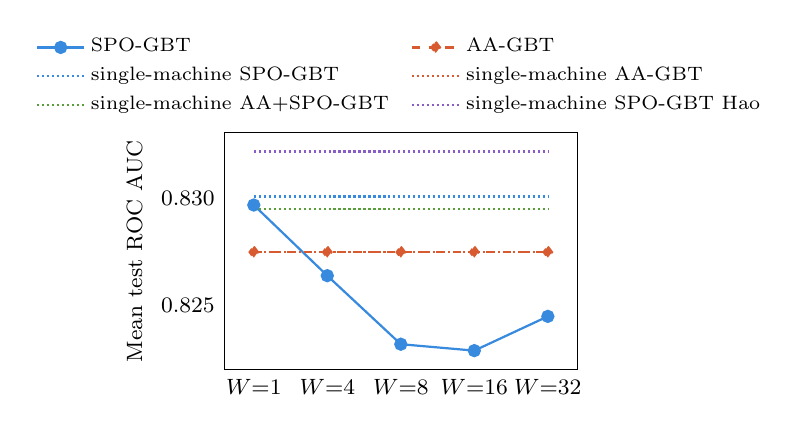
\begin{tikzpicture}
\begin{axis}[width=0.5\textwidth, height=4.6cm, ymin=0.8220, ymax=0.8331, symbolic x coords={1,4,8,16,32}, xtick=data,
  xticklabels={$W{=}1$,$W{=}4$,$W{=}8$,$W{=}16$,$W{=}32$}, ylabel={Mean test ROC AUC},
  yticklabel style={/pgf/number format/fixed, /pgf/number format/precision=3, /pgf/number format/fixed zerofill},
  tick label style={font=\footnotesize}, label style={font=\footnotesize}, tick style={draw=none},
  legend style={font=\scriptsize, at={(0.5,1.03)}, anchor=south, draw=none, /tikz/every even column/.append style={column sep=6pt}}, legend columns=2, legend cell align=left]
\addplot[color={rgb,255:red,55;green,138;blue,221}, mark=*, thick] coordinates {(1,0.8297) (4,0.8264) (8,0.8232) (16,0.8229) (32,0.8245)};
\addlegendentry{SPO-GBT}
\addplot[color={rgb,255:red,216;green,90;blue,48}, mark=diamond*, thick, dashed] coordinates {(1,0.8275) (4,0.8275) (8,0.8275) (16,0.8275) (32,0.8275)};
\addlegendentry{AA-GBT}
\addplot[color={rgb,255:red,55;green,138;blue,221}, thick, densely dotted, no marks] coordinates {(1,0.8301) (32,0.8301)};
\addlegendentry{single-machine SPO-GBT}
\addplot[color={rgb,255:red,216;green,90;blue,48}, thick, densely dotted, no marks] coordinates {(1,0.8275) (32,0.8275)};
\addlegendentry{single-machine AA-GBT}
\addplot[color={rgb,255:red,90;green,158;blue,60}, thick, densely dotted, no marks] coordinates {(1,0.8295) (32,0.8295)};
\addlegendentry{single-machine AA+SPO-GBT}
\addplot[color={rgb,255:red,138;green,92;blue,200}, thick, densely dotted, no marks] coordinates {(1,0.8322) (32,0.8322)};
\addlegendentry{single-machine SPO-GBT Hao}
\end{axis}
\end{tikzpicture}
}{\TODO{rerun pending: profile kdd28\_ydf}}\end{minipage}}
\caption{Mean test AUC over the datasets of Table~\ref{tab:dist-accuracy-ydf}. \textcolor{RoyalPurple}{*Some datasets have few columns, so as $W$ increases, accuracy actually approaches} \textcolor{red}{AA-GBT}}
\Description{Line chart of mean AUC versus number of workers for SPO-GBT and AA-GBT.}
\label{fig:dist-accuracy-mean-ydf}
\end{minipage}\hfill
\begin{minipage}[t]{0.48\textwidth}\vspace{0pt}
\captionsetup{type=figure}
\centering
\resizebox{\linewidth}{!}{\begin{minipage}{1.25\linewidth}\IfFileExists{figures/evaluation/fig_column_replication_ydf_body.tex}{% auto-generated by benchmarks/src/distributed_spo_gbt/make_column_replication_fig.py -- regenerate, do not hand-edit
% setup: 300 trees, depth 6, EXACT, P=min(F^2,6000) total over W, density 2, no early stopping, W=4, CC18 fold 0, seeds 1-5 (profile kdd28_ydf) | distacc_single_spo: P=min(F^2,6000), single machine, 5 CV folds (chronological sets: 1 holdout), seed 1 | colrep_distacc_spo: 5 CV folds (chronological sets: 1 holdout), seed 1 | distacc_spo: W=1/4/8/16/32, 5 CV folds (chronological sets: 1 holdout), seed 1 | eval suite kdd28_tabarena33
\begin{tikzpicture}
\begin{groupplot}[group style={group size=1 by 2, vertical sep=0.35cm, xticklabels at=edge bottom, xlabels at=edge bottom},
  width=\linewidth, xmin=-0.05, xmax=1.05, xtick={0,0.1,...,1.0},
  xticklabel style={/pgf/number format/fixed, /pgf/number format/precision=1, /pgf/number format/fixed zerofill},
  xlabel={column replication $r$}, tick label style={font=\footnotesize}, label style={font=\footnotesize},
  tick style={draw=none}, ymajorgrids, grid style={gray!25}, axis line style={gray!70}, every axis plot/.append style={line join=round}]
\nextgroupplot[height=3.6cm, ylabel={$\Delta$ mean AUC (pts)}]
\addplot[draw=none, fill={rgb,255:red,55;green,138;blue,221}, fill opacity=0.18, forget plot] table {figures/evaluation/column_replication_ydf/band.dat};
\addplot[color={rgb,255:red,0;green,131;blue,0}, dashed, forget plot] coordinates {(-0.05,0) (1.05,0)};
\node[font=\scriptsize, text={rgb,255:red,0;green,131;blue,0}, anchor=south east] at (axis cs:1.05,0) {single};
\addplot[color={rgb,255:red,55;green,138;blue,221}, mark=*, mark size=1.5pt, thick] table[x=r, y=mean] {figures/evaluation/column_replication_ydf/mean.dat};
\nextgroupplot[height=4.2cm, ymin=-5, ymax=5, ytick={-4,-2,...,4}, ylabel={per-dataset $\Delta$ (pts)}]
\addplot[color={rgb,255:red,0;green,131;blue,0}, dashed, forget plot] coordinates {(-0.05,0) (1.05,0)};
\addplot[only marks, mark=*, mark size=0.6pt, color={rgb,255:red,55;green,138;blue,221}, opacity=0.45] table[x=x, y=d] {figures/evaluation/column_replication_ydf/dots.dat};
\addplot[gray!90, empty line=jump] table {figures/evaluation/column_replication_ydf/boxes.dat};
\addplot[black, thick, empty line=jump] table {figures/evaluation/column_replication_ydf/medians.dat};
\addplot[color={rgb,255:red,216;green,90;blue,48}, mark=diamond*, mark size=1.6pt] table[x=r, y=mean] {figures/evaluation/column_replication_ydf/mean.dat};
\end{groupplot}
\end{tikzpicture}
}{\TODO{rerun pending: profile kdd28\_ydf}}\end{minipage}}
\caption{Table~\ref{tab:column-replication-ydf} as charts: mean (top) and per-dataset (bottom) $\Delta$ test accuracy at \texttt{MULTI\_THREAD} $W=4$ vs.\ \texttt{single}.}
\Description{Two stacked panels sharing the replication axis r from 0 to 1. Top: line of the mean accuracy difference to r equals 0 with a shaded confidence band. Bottom: one box plot of per-dataset differences per r, overlaid with the dataset points and the mean. A separate green slot labelled single, right of a dotted line, shows single-machine SPO-GBT the same way, with a dashed line at its mean in the top panel.}
\label{fig:column-replication-ydf}
\par\smallskip\raggedright\footnotesize Top: 95\% bootstrap interval over the datasets. Bottom: per-dataset $\Delta$ (dots) with box plots and the mean (diamonds). \textcolor{green}{Green (\texttt{single})}: single-machine SPO-GBT accuracy. pts = percentage points of test accuracy.
\end{minipage}
}]

\twocolumn[{\floatblock
\section{Accuracy on Datasets with >100 Columns}
\label{sec:accuracy-wide}

\mbox{}\par\vskip0.5em
\noindent\begin{minipage}{\textwidth}
\captionsetup{type=table}
\centering
\scriptsize
\setlength{\tabcolsep}{2pt}
\caption{Test AUC of single-machine vs. $W$-distributed GBT on the datasets with $F>100$.}
\label{tab:dist-accuracy-ydf-wide}
\IfFileExists{tables/table_dist_accuracy_ydf_wide_body.tex}{% auto-generated by benchmarks/src/distributed_spo_gbt/make_paper_tables.py -- regenerate, do not hand-edit
% source: IN-PROCESS reruns (workers = threads of one process): SPAA paper eval rows on AWS m7i.metal-24xl, wide dataset eval rows on c8i.metal-96xl; datasets with F>=100, results/kdd28/accuracy/tab-dist-accuracy-ydf-wide/union/distacc/results.csv + results/kdd28/accuracy/tab-dist-accuracy-ydf-wide/union/distacc_aaspo/results.csv + results/kdd28/accuracy/tab-dist-accuracy-ydf-wide/union/distacc_exact300/results.csv
% setup: 300 trees, depth 6, EXACT (profile kdd28_ydf) | distacc_single_spo: P=min(F^2,6000), density 2, no early stopping, single machine, 5 CV folds (chronological sets: 1 holdout), seed 1 | distacc_single_aa: P=n/a (AA), no early stopping, single machine, 5 CV folds (chronological sets: 1 holdout), seed 1 | distacc_spo: P=min(F^2,6000) total over W, density 2, W=1/4/8/16/32, 5 CV folds (chronological sets: 1 holdout), seed 1 | distacc_aa: P=n/a (AA), W=1/4/8/16/32, 5 CV folds (chronological sets: 1 holdout), seed 1 | distacc_single_aa_spo: P=min(F^2,6000), density 2, + axis-aligned splits, no early stopping, single machine, 5 CV folds (chronological sets: 1 holdout), seed 1 | distacc_single_spo_harness_exact300: P=min(F,1000), density 1.5, no early stopping, single machine, 5 CV folds (chronological sets: 1 holdout), seed 1 | eval suite kdd28_wide_union

\resizebox{\linewidth}{!}{%
\begin{tabular}{lr|r|rrrrrr|rrrrrr}
\toprule
Dataset & \multicolumn{1}{c}{\parbox[b]{1.0cm}{\centering AA+SPO-GBT single machine}} & \multicolumn{1}{c}{\parbox[b]{1.0cm}{\centering SPO-GBT Hao single machine}} & \multicolumn{1}{c}{\parbox[b]{1.0cm}{\centering SPO-GBT single machine}} & \multicolumn{1}{c}{\parbox[b]{1.0cm}{\centering SPO-GBT dist.\ $W{=}1$}} & \multicolumn{1}{c}{\parbox[b]{1.0cm}{\centering SPO-GBT dist.\ $W{=}4$}} & \multicolumn{1}{c}{\parbox[b]{1.0cm}{\centering SPO-GBT dist.\ $W{=}8$}} & \multicolumn{1}{c}{\parbox[b]{1.0cm}{\centering SPO-GBT dist.\ $W{=}16$}} & \multicolumn{1}{c}{\parbox[b]{1.0cm}{\centering SPO-GBT dist.\ $W{=}32$}} & \multicolumn{1}{c}{\parbox[b]{1.0cm}{\centering AA-GBT single machine}} & \multicolumn{1}{c}{\parbox[b]{1.0cm}{\centering AA-GBT dist.\ $W{=}1$}} & \multicolumn{1}{c}{\parbox[b]{1.0cm}{\centering AA-GBT dist.\ $W{=}4$}} & \multicolumn{1}{c}{\parbox[b]{1.0cm}{\centering AA-GBT dist.\ $W{=}8$}} & \multicolumn{1}{c}{\parbox[b]{1.0cm}{\centering AA-GBT dist.\ $W{=}16$}} & \multicolumn{1}{c}{\parbox[b]{1.0cm}{\centering AA-GBT dist.\ $W{=}32$}} \\
\midrule
APSFailure (76k, 170) & {\boldmath\textbf{.9916$_{\pm.0039}$}} & .9915$_{\pm.0037}$ & .9914$_{\pm.0045}$ & \cellcolor[RGB]{240,239,236}.9914$_{\pm.0041}$ & \cellcolor[RGB]{240,237,234}.9912$_{\pm.0032}$ & \cellcolor[RGB]{240,236,233}.9912$_{\pm.0032}$ & \cellcolor[RGB]{240,237,234}.9913$_{\pm.0041}$ & \cellcolor[RGB]{239,230,227}.9906$_{\pm.0034}$ & .9902$_{\pm.0040}$ & \cellcolor[RGB]{240,234,231}.9898$_{\pm.0040}$ & \cellcolor[RGB]{240,234,231}.9898$_{\pm.0040}$ & \cellcolor[RGB]{240,234,231}.9898$_{\pm.0040}$ & \cellcolor[RGB]{240,234,231}.9898$_{\pm.0040}$ & \cellcolor[RGB]{240,234,231}.9898$_{\pm.0040}$ \\
Bioresponse (3751, 1776) & .8733$_{\pm.0101}$ & .8725$_{\pm.0120}$ & .8722$_{\pm.0101}$ & \cellcolor[RGB]{208,220,232}{\boldmath\textbf{.8746$_{\pm.0125}$}} & \cellcolor[RGB]{220,227,234}.8737$_{\pm.0087}$ & \cellcolor[RGB]{225,230,234}.8733$_{\pm.0098}$ & \cellcolor[RGB]{236,237,236}.8725$_{\pm.0106}$ & \cellcolor[RGB]{215,224,233}.8740$_{\pm.0104}$ & .8698$_{\pm.0067}$ & \cellcolor[RGB]{230,233,235}.8706$_{\pm.0082}$ & \cellcolor[RGB]{230,233,235}.8706$_{\pm.0082}$ & \cellcolor[RGB]{230,233,235}.8706$_{\pm.0082}$ & \cellcolor[RGB]{230,233,235}.8706$_{\pm.0082}$ & \cellcolor[RGB]{230,233,235}.8706$_{\pm.0082}$ \\
christine (5418, 1636) & .8204$_{\pm.0138}$ & .8192$_{\pm.0109}$ & .8196$_{\pm.0104}$ & \cellcolor[RGB]{237,237,236}.8198$_{\pm.0148}$ & \cellcolor[RGB]{225,230,234}.8207$_{\pm.0104}$ & \cellcolor[RGB]{238,209,206}.8168$_{\pm.0130}$ & \cellcolor[RGB]{238,210,208}.8170$_{\pm.0124}$ & \cellcolor[RGB]{224,230,234}{\boldmath\textbf{.8208$_{\pm.0107}$}} & .8149$_{\pm.0126}$ & \cellcolor[RGB]{239,230,227}.8141$_{\pm.0121}$ & \cellcolor[RGB]{239,230,227}.8141$_{\pm.0121}$ & \cellcolor[RGB]{239,230,227}.8141$_{\pm.0121}$ & \cellcolor[RGB]{239,230,227}.8141$_{\pm.0121}$ & \cellcolor[RGB]{239,230,227}.8141$_{\pm.0121}$ \\
dota2 (103k, 116) & .6285$_{\pm.0043}$ & {\boldmath\textbf{.6306$_{\pm.0048}$}} & .6283$_{\pm.0039}$ & \cellcolor[RGB]{218,226,234}.6299$_{\pm.0026}$ & \cellcolor[RGB]{238,238,236}.6284$_{\pm.0041}$ & \cellcolor[RGB]{238,217,214}.6262$_{\pm.0034}$ & \cellcolor[RGB]{237,206,203}.6253$_{\pm.0048}$ & \cellcolor[RGB]{238,217,214}.6263$_{\pm.0046}$ & .6285$_{\pm.0041}$ & \cellcolor[RGB]{240,238,235}.6284$_{\pm.0041}$ & \cellcolor[RGB]{240,238,235}.6284$_{\pm.0041}$ & \cellcolor[RGB]{240,238,235}.6284$_{\pm.0041}$ & \cellcolor[RGB]{240,238,235}.6284$_{\pm.0041}$ & \cellcolor[RGB]{240,238,235}.6284$_{\pm.0041}$ \\
ecom-offers (40k, 119) & .6166\phantom{$_{\pm.0000}$} & .6141\phantom{$_{\pm.0000}$} & .6126\phantom{$_{\pm.0000}$} & \cellcolor[RGB]{215,224,233}.6145\phantom{$_{\pm.0000}$} & \cellcolor[RGB]{238,209,206}.6099\phantom{$_{\pm.0000}$} & \cellcolor[RGB]{240,237,234}.6124\phantom{$_{\pm.0000}$} & \cellcolor[RGB]{202,216,232}.6155\phantom{$_{\pm.0000}$} & \cellcolor[RGB]{194,211,231}.6161\phantom{$_{\pm.0000}$} & \textbf{.6197}\phantom{$_{\pm.0000}$} & \cellcolor[RGB]{239,230,227}.6189\phantom{$_{\pm.0000}$} & \cellcolor[RGB]{239,230,227}.6189\phantom{$_{\pm.0000}$} & \cellcolor[RGB]{239,230,227}.6189\phantom{$_{\pm.0000}$} & \cellcolor[RGB]{239,230,227}.6189\phantom{$_{\pm.0000}$} & \cellcolor[RGB]{239,230,227}.6189\phantom{$_{\pm.0000}$} \\
epsilon (500k, 2000) & \textbf{.9518}\phantom{$_{\pm.0000}$} & .9465\phantom{$_{\pm.0000}$} & .9510\phantom{$_{\pm.0000}$} & \cellcolor[RGB]{240,238,235}.9510\phantom{$_{\pm.0000}$} & \cellcolor[RGB]{240,235,232}.9506\phantom{$_{\pm.0000}$} & \cellcolor[RGB]{239,230,227}.9502\phantom{$_{\pm.0000}$} & \cellcolor[RGB]{239,225,222}.9498\phantom{$_{\pm.0000}$} & \cellcolor[RGB]{238,218,215}.9491\phantom{$_{\pm.0000}$} & .9403\phantom{$_{\pm.0000}$} & \cellcolor[RGB]{240,239,236}.9403\phantom{$_{\pm.0000}$} & \cellcolor[RGB]{240,239,236}.9403\phantom{$_{\pm.0000}$} & \cellcolor[RGB]{240,239,236}.9403\phantom{$_{\pm.0000}$} & \cellcolor[RGB]{240,239,236}.9403\phantom{$_{\pm.0000}$} & \cellcolor[RGB]{240,239,236}.9403\phantom{$_{\pm.0000}$} \\
guillermo (20k, 4296) & .9019$_{\pm.0046}$ & .8981$_{\pm.0046}$ & .8998$_{\pm.0044}$ & \cellcolor[RGB]{240,236,233}.8995$_{\pm.0045}$ & \cellcolor[RGB]{239,232,229}.8992$_{\pm.0051}$ & \cellcolor[RGB]{239,225,222}.8986$_{\pm.0061}$ & \cellcolor[RGB]{233,235,235}.9004$_{\pm.0053}$ & \cellcolor[RGB]{219,227,234}.9014$_{\pm.0045}$ & {\boldmath\textbf{.9027$_{\pm.0046}$}} & \cellcolor[RGB]{239,230,227}.9018$_{\pm.0039}$ & \cellcolor[RGB]{239,230,227}.9018$_{\pm.0039}$ & \cellcolor[RGB]{239,230,227}.9018$_{\pm.0039}$ & \cellcolor[RGB]{239,230,227}.9018$_{\pm.0039}$ & \cellcolor[RGB]{239,230,227}.9018$_{\pm.0039}$ \\
hcdr\_main (308k, 120) & .7553$_{\pm.0037}$ & .7575$_{\pm.0039}$ & .7558$_{\pm.0042}$ & \cellcolor[RGB]{240,235,232}.7554$_{\pm.0041}$ & \cellcolor[RGB]{238,214,212}.7535$_{\pm.0037}$ & \cellcolor[RGB]{239,224,221}.7544$_{\pm.0036}$ & \cellcolor[RGB]{239,225,222}.7545$_{\pm.0038}$ & \cellcolor[RGB]{240,239,236}.7558$_{\pm.0038}$ & .7579$_{\pm.0031}$ & \cellcolor[RGB]{240,239,236}{\boldmath\textbf{.7579$_{\pm.0031}$}} & \cellcolor[RGB]{240,239,236}{\boldmath\textbf{.7579$_{\pm.0031}$}} & \cellcolor[RGB]{240,239,236}{\boldmath\textbf{.7579$_{\pm.0031}$}} & \cellcolor[RGB]{240,239,236}{\boldmath\textbf{.7579$_{\pm.0031}$}} & \cellcolor[RGB]{240,239,236}{\boldmath\textbf{.7579$_{\pm.0031}$}} \\
homecredit-default (40k, 696) & .7986\phantom{$_{\pm.0000}$} & \textbf{.8151}\phantom{$_{\pm.0000}$} & .8092\phantom{$_{\pm.0000}$} & \cellcolor[RGB]{227,73,72}\color{white}.7816\phantom{$_{\pm.0000}$} & \cellcolor[RGB]{227,73,72}\color{white}.7744\phantom{$_{\pm.0000}$} & \cellcolor[RGB]{227,73,72}\color{white}.7685\phantom{$_{\pm.0000}$} & \cellcolor[RGB]{227,73,72}\color{white}.7914\phantom{$_{\pm.0000}$} & \cellcolor[RGB]{227,73,72}\color{white}.7568\phantom{$_{\pm.0000}$} & .8061\phantom{$_{\pm.0000}$} & \cellcolor[RGB]{225,230,234}.8072\phantom{$_{\pm.0000}$} & \cellcolor[RGB]{225,230,234}.8072\phantom{$_{\pm.0000}$} & \cellcolor[RGB]{225,230,234}.8072\phantom{$_{\pm.0000}$} & \cellcolor[RGB]{225,230,234}.8072\phantom{$_{\pm.0000}$} & \cellcolor[RGB]{225,230,234}.8072\phantom{$_{\pm.0000}$} \\
homesite-insurance (40k, 299) & .9546\phantom{$_{\pm.0000}$} & .9544\phantom{$_{\pm.0000}$} & .9531\phantom{$_{\pm.0000}$} & \cellcolor[RGB]{217,225,233}.9548\phantom{$_{\pm.0000}$} & \cellcolor[RGB]{233,235,235}.9536\phantom{$_{\pm.0000}$} & \cellcolor[RGB]{236,237,236}.9534\phantom{$_{\pm.0000}$} & \cellcolor[RGB]{239,222,219}.9515\phantom{$_{\pm.0000}$} & \cellcolor[RGB]{239,228,225}.9521\phantom{$_{\pm.0000}$} & .9551\phantom{$_{\pm.0000}$} & \cellcolor[RGB]{239,238,236}\textbf{.9552}\phantom{$_{\pm.0000}$} & \cellcolor[RGB]{239,238,236}\textbf{.9552}\phantom{$_{\pm.0000}$} & \cellcolor[RGB]{239,238,236}\textbf{.9552}\phantom{$_{\pm.0000}$} & \cellcolor[RGB]{239,238,236}\textbf{.9552}\phantom{$_{\pm.0000}$} & \cellcolor[RGB]{239,238,236}\textbf{.9552}\phantom{$_{\pm.0000}$} \\
kddcup09\_appetency (50k, 212) & .8002$_{\pm.0097}$ & {\boldmath\textbf{.8053$_{\pm.0079}$}} & .8002$_{\pm.0084}$ & \cellcolor[RGB]{239,228,225}.7992$_{\pm.0146}$ & \cellcolor[RGB]{219,226,234}.8018$_{\pm.0146}$ & \cellcolor[RGB]{209,220,233}.8025$_{\pm.0145}$ & \cellcolor[RGB]{239,228,225}.7992$_{\pm.0180}$ & \cellcolor[RGB]{237,204,202}.7970$_{\pm.0105}$ & .8035$_{\pm.0111}$ & \cellcolor[RGB]{235,236,235}.8039$_{\pm.0134}$ & \cellcolor[RGB]{235,236,235}.8039$_{\pm.0134}$ & \cellcolor[RGB]{235,236,235}.8039$_{\pm.0134}$ & \cellcolor[RGB]{235,236,235}.8039$_{\pm.0134}$ & \cellcolor[RGB]{235,236,235}.8039$_{\pm.0134}$ \\
philippine (5832, 308) & {\boldmath\textbf{.8711$_{\pm.0156}$}} & .8639$_{\pm.0147}$ & .8702$_{\pm.0145}$ & \cellcolor[RGB]{239,228,225}.8692$_{\pm.0154}$ & \cellcolor[RGB]{240,233,230}.8697$_{\pm.0158}$ & \cellcolor[RGB]{234,165,163}.8636$_{\pm.0131}$ & \cellcolor[RGB]{233,145,143}.8617$_{\pm.0146}$ & \cellcolor[RGB]{227,73,72}\color{white}.8541$_{\pm.0122}$ & .8540$_{\pm.0173}$ & \cellcolor[RGB]{237,206,203}.8510$_{\pm.0187}$ & \cellcolor[RGB]{237,206,203}.8510$_{\pm.0187}$ & \cellcolor[RGB]{237,206,203}.8510$_{\pm.0187}$ & \cellcolor[RGB]{237,206,203}.8510$_{\pm.0187}$ & \cellcolor[RGB]{237,206,203}.8510$_{\pm.0187}$ \\
santander\_transaction (200k, 200) & .8814$_{\pm.0020}$ & {\boldmath\textbf{.8844$_{\pm.0027}$}} & .8823$_{\pm.0019}$ & \cellcolor[RGB]{240,235,232}.8819$_{\pm.0019}$ & \cellcolor[RGB]{239,221,218}.8806$_{\pm.0023}$ & \cellcolor[RGB]{237,205,202}.8792$_{\pm.0012}$ & \cellcolor[RGB]{237,202,199}.8789$_{\pm.0019}$ & \cellcolor[RGB]{237,199,197}.8787$_{\pm.0029}$ & .8806$_{\pm.0028}$ & \cellcolor[RGB]{239,239,236}.8806$_{\pm.0032}$ & \cellcolor[RGB]{239,239,236}.8806$_{\pm.0032}$ & \cellcolor[RGB]{239,239,236}.8806$_{\pm.0032}$ & \cellcolor[RGB]{239,239,236}.8806$_{\pm.0032}$ & \cellcolor[RGB]{239,239,236}.8806$_{\pm.0032}$ \\
vehicle\_sensIT (99k, 100) & {\boldmath\textbf{.9291$_{\pm.0019}$}} & .9286$_{\pm.0018}$ & .9289$_{\pm.0015}$ & \cellcolor[RGB]{240,234,231}.9284$_{\pm.0019}$ & \cellcolor[RGB]{239,232,229}.9283$_{\pm.0018}$ & \cellcolor[RGB]{239,220,217}.9272$_{\pm.0021}$ & \cellcolor[RGB]{237,207,204}.9260$_{\pm.0021}$ & \cellcolor[RGB]{237,197,194}.9251$_{\pm.0021}$ & .9253$_{\pm.0013}$ & \cellcolor[RGB]{240,239,236}.9253$_{\pm.0013}$ & \cellcolor[RGB]{240,239,236}.9253$_{\pm.0013}$ & \cellcolor[RGB]{240,239,236}.9253$_{\pm.0013}$ & \cellcolor[RGB]{240,239,236}.9253$_{\pm.0013}$ & \cellcolor[RGB]{240,239,236}.9253$_{\pm.0013}$ \\
\midrule
Mean & .8410\phantom{$_{\pm.0000}$} & \textbf{.8415}\phantom{$_{\pm.0000}$} & .8410\phantom{$_{\pm.0000}$} & \cellcolor[RGB]{239,221,219}.8394\phantom{$_{\pm.0000}$} & \cellcolor[RGB]{238,209,206}.8383\phantom{$_{\pm.0000}$} & \cellcolor[RGB]{237,195,192}.8370\phantom{$_{\pm.0000}$} & \cellcolor[RGB]{238,208,205}.8382\phantom{$_{\pm.0000}$} & \cellcolor[RGB]{235,179,177}.8356\phantom{$_{\pm.0000}$} & .8392\phantom{$_{\pm.0000}$} & \cellcolor[RGB]{240,236,233}.8389\phantom{$_{\pm.0000}$} & \cellcolor[RGB]{240,236,233}.8389\phantom{$_{\pm.0000}$} & \cellcolor[RGB]{240,236,233}.8389\phantom{$_{\pm.0000}$} & \cellcolor[RGB]{240,236,233}.8389\phantom{$_{\pm.0000}$} & \cellcolor[RGB]{240,236,233}.8389\phantom{$_{\pm.0000}$} \\
\bottomrule
\end{tabular}}
}{\TODO{rerun pending: profile kdd28\_ydf}}
\par\smallskip\raggedright\footnotesize Datasets of Table~\ref{tab:dist-accuracy-ydf} with $F>100$. YDF defaults, early stopping off, 300 trees, depth 6, $P{=}\min(F^2,6000)$ split across workers. 5 CV folds except Chronological holdouts.
\end{minipage}
\par\vskip0.5em
\noindent\begin{minipage}[t]{0.48\textwidth}\vspace{0pt}
\captionsetup{type=figure}
\centering
% body sizes its axis to 0.5\textwidth; match it to the column
\resizebox{\linewidth}{!}{\begin{minipage}{1.2\linewidth}\setlength{\textwidth}{2\linewidth}%
\IfFileExists{figures/evaluation/fig_dist_accuracy_mean_ydf_wide_body.tex}{% auto-generated by benchmarks/src/distributed_spo_gbt/make_paper_tables.py -- regenerate, do not hand-edit
% source: IN-PROCESS rerun on AWS m7i.metal-24xl (Xeon 8488C; workers = threads of one process), datasets with F>100, results/kdd28/accuracy/tab-dist-accuracy-ydf-wide/distacc/results.csv + results/kdd28/accuracy/tab-dist-accuracy-ydf-wide/distacc_aaspo/distacc_aaspo.csv + results/kdd28/accuracy/tab-dist-accuracy-ydf-wide/distacc_aaspo/distacc_exact300.csv
% setup: 300 trees, depth 6, EXACT, P=min(F^2,6000) total over W, density 2, no early stopping, W=4, CC18 fold 0, seeds 1-5 (profile kdd28_ydf) | distacc_single_spo: P=min(F^2,6000), single machine, 5 CV folds (chronological sets: 1 holdout), seed 1 | distacc_single_aa: P=n/a (AA), single machine, 5 CV folds (chronological sets: 1 holdout), seed 1 | distacc_spo: W=1/4/8/16/32, 5 CV folds (chronological sets: 1 holdout), seed 1 | distacc_aa: P=n/a (AA), W=1/4/8/16/32, 5 CV folds (chronological sets: 1 holdout), seed 1 | eval suite kdd28_tabarena33

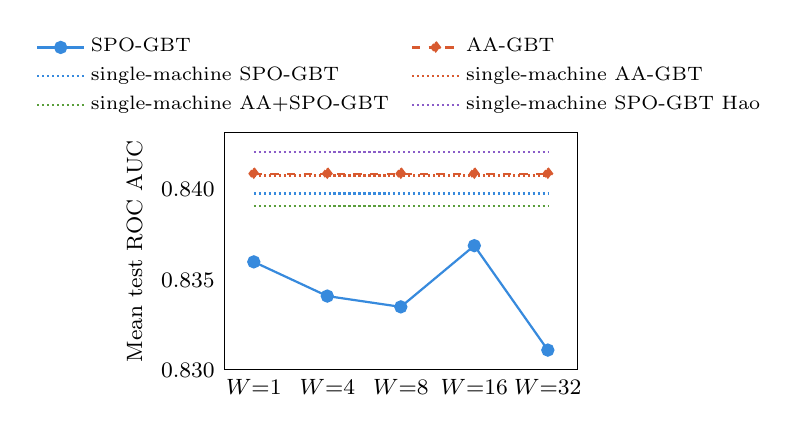
\begin{tikzpicture}
\begin{axis}[width=0.5\textwidth, height=4.6cm, ymin=0.8300, ymax=0.8432, symbolic x coords={1,4,8,16,32}, xtick=data,
  xticklabels={$W{=}1$,$W{=}4$,$W{=}8$,$W{=}16$,$W{=}32$}, ylabel={Mean test ROC AUC},
  yticklabel style={/pgf/number format/fixed, /pgf/number format/precision=3, /pgf/number format/fixed zerofill},
  tick label style={font=\footnotesize}, label style={font=\footnotesize}, tick style={draw=none},
  legend style={font=\scriptsize, at={(0.5,1.03)}, anchor=south, draw=none, /tikz/every even column/.append style={column sep=6pt}}, legend columns=2, legend cell align=left]
\addplot[color={rgb,255:red,55;green,138;blue,221}, mark=*, thick] coordinates {(1,0.8360) (4,0.8341) (8,0.8335) (16,0.8369) (32,0.8311)};
\addlegendentry{SPO-GBT}
\addplot[color={rgb,255:red,216;green,90;blue,48}, mark=diamond*, thick, dashed] coordinates {(1,0.8409) (4,0.8409) (8,0.8409) (16,0.8409) (32,0.8409)};
\addlegendentry{AA-GBT}
\addplot[color={rgb,255:red,55;green,138;blue,221}, thick, densely dotted, no marks] coordinates {(1,0.8398) (32,0.8398)};
\addlegendentry{single-machine SPO-GBT}
\addplot[color={rgb,255:red,216;green,90;blue,48}, thick, densely dotted, no marks] coordinates {(1,0.8408) (32,0.8408)};
\addlegendentry{single-machine AA-GBT}
\addplot[color={rgb,255:red,90;green,158;blue,60}, thick, densely dotted, no marks] coordinates {(1,0.8391) (32,0.8391)};
\addlegendentry{single-machine AA+SPO-GBT}
\addplot[color={rgb,255:red,138;green,92;blue,200}, thick, densely dotted, no marks] coordinates {(1,0.8421) (32,0.8421)};
\addlegendentry{single-machine SPO-GBT Hao}
\end{axis}
\end{tikzpicture}
}{\TODO{rerun pending: profile kdd28\_ydf}}\end{minipage}}
\caption{Mean test AUC over the datasets of Table~\ref{tab:dist-accuracy-ydf-wide}.}
\Description{Line chart of mean AUC versus number of workers for SPO-GBT and AA-GBT on the datasets with more than 100 columns.}
\label{fig:dist-accuracy-mean-ydf-wide}
\end{minipage}\hfill
\begin{minipage}[t]{0.48\textwidth}\vspace{0pt}
\captionsetup{type=figure}
\centering
\resizebox{\linewidth}{!}{\begin{minipage}{1.25\linewidth}\IfFileExists{figures/evaluation/fig_column_replication_ydf_wide_body.tex}{% auto-generated by benchmarks/src/distributed_spo_gbt/make_column_replication_fig.py -- regenerate, do not hand-edit
% setup: 300 trees, depth 6, EXACT, P=min(F^2,6000) total over W, density 2, no early stopping, W=4, CC18 fold 0, seeds 1-5 (profile kdd28_ydf) | distacc_single_spo: P=min(F^2,6000), single machine, 5 CV folds (chronological sets: 1 holdout), seed 1 | colrep_distacc_spo: 5 CV folds (chronological sets: 1 holdout), seed 1 | distacc_spo: W=1/4/8/16/32, 5 CV folds (chronological sets: 1 holdout), seed 1 | eval suite kdd28_tabarena33
\begin{tikzpicture}
\begin{groupplot}[group style={group size=1 by 2, vertical sep=0.35cm, xticklabels at=edge bottom, xlabels at=edge bottom},
  width=\linewidth, xmin=-0.05, xmax=1.05, xtick={0,0.1,...,1.0},
  xticklabel style={/pgf/number format/fixed, /pgf/number format/precision=1, /pgf/number format/fixed zerofill},
  xlabel={column replication $r$}, tick label style={font=\footnotesize}, label style={font=\footnotesize},
  tick style={draw=none}, ymajorgrids, grid style={gray!25}, axis line style={gray!70}, every axis plot/.append style={line join=round}]
\nextgroupplot[height=3.6cm, ylabel={$\Delta$ mean AUC (pts)}]
\addplot[draw=none, fill={rgb,255:red,55;green,138;blue,221}, fill opacity=0.18, forget plot] table {figures/evaluation/column_replication_ydf_wide/band.dat};
\addplot[color={rgb,255:red,0;green,131;blue,0}, dashed, forget plot] coordinates {(-0.05,0) (1.05,0)};
\node[font=\scriptsize, text={rgb,255:red,0;green,131;blue,0}, anchor=south east] at (axis cs:1.05,0) {single};
\addplot[color={rgb,255:red,55;green,138;blue,221}, mark=*, mark size=1.5pt, thick] table[x=r, y=mean] {figures/evaluation/column_replication_ydf_wide/mean.dat};
\nextgroupplot[height=4.2cm, ymin=-5, ymax=5, ytick={-4,-2,...,4}, ylabel={per-dataset $\Delta$ (pts)}]
\addplot[color={rgb,255:red,0;green,131;blue,0}, dashed, forget plot] coordinates {(-0.05,0) (1.05,0)};
\addplot[only marks, mark=*, mark size=0.6pt, color={rgb,255:red,55;green,138;blue,221}, opacity=0.45] table[x=x, y=d] {figures/evaluation/column_replication_ydf_wide/dots.dat};
\addplot[gray!90, empty line=jump] table {figures/evaluation/column_replication_ydf_wide/boxes.dat};
\addplot[black, thick, empty line=jump] table {figures/evaluation/column_replication_ydf_wide/medians.dat};
\addplot[color={rgb,255:red,216;green,90;blue,48}, mark=diamond*, mark size=1.6pt] table[x=r, y=mean] {figures/evaluation/column_replication_ydf_wide/mean.dat};
\end{groupplot}
\end{tikzpicture}
}{\TODO{rerun pending: profile kdd28\_ydf}}\end{minipage}}
\caption{Table~\ref{tab:column-replication-ydf-wide} as charts: mean (top) and per-dataset (bottom) $\Delta$ test accuracy at \texttt{MULTI\_THREAD} $W=4$ vs.\ \texttt{single}.}
\Description{Two stacked panels sharing the replication axis r from 0 to 1, for the datasets with more than 100 columns. Top: line of the mean accuracy difference to r equals 0 with a shaded confidence band. Bottom: one box plot of per-dataset differences per r, overlaid with the dataset points and the mean. A separate green slot labelled single, right of a dotted line, shows single-machine SPO-GBT the same way, with a dashed line at its mean in the top panel.}
\label{fig:column-replication-ydf-wide}
\par\smallskip\raggedright\footnotesize Top: 95\% bootstrap interval over the datasets. Bottom: per-dataset $\Delta$ (dots) with box plots and the mean (diamonds). \textcolor{green}{Green (\texttt{single})}: single-machine SPO-GBT accuracy. pts = percentage points of test accuracy.
\end{minipage}
\par\vskip0.5em
\noindent\begin{minipage}{\textwidth}
\captionsetup{type=table}
\centering\footnotesize\setlength{\tabcolsep}{3pt}
\caption{Test accuracy of distributed SPO-GBT vs.\ column replication $r$ on the datasets with $F>100$.}
\label{tab:column-replication-ydf-wide}
\IfFileExists{tables/table_column_replication_ydf_wide_body.tex}{% auto-generated by benchmarks/src/distributed_spo_gbt/make_column_replication_table.py -- regenerate, do not hand-edit
% data: benchmarks/results/kdd28/accuracy/tab-dist-accuracy-ydf-wide/colrep_distacc/results.csv (IN-PROCESS rerun, c8i.metal-96xl SMT+turbo, W=4; r=0 and single = 2026-11-03 m7i distacc rows; datasets with F>100); single: benchmarks/results/kdd28/accuracy/tab-dist-accuracy-ydf-wide/distacc/results.csv (arm=single:SPO); r = 0: benchmarks/results/kdd28/accuracy/tab-dist-accuracy-ydf-wide/distacc/results.csv (arm=4:SPO)
% setup: 300 trees, depth 6, EXACT, P=min(F^2,6000) total over W, density 2, no early stopping, W=4, CC18 fold 0, seeds 1-5 (profile kdd28_ydf) | distacc_single_spo: P=min(F^2,6000), single machine, 5 CV folds (chronological sets: 1 holdout), seed 1 | colrep_distacc_spo: 5 CV folds (chronological sets: 1 holdout), seed 1 | distacc_spo: W=1/4/8/16/32, 5 CV folds (chronological sets: 1 holdout), seed 1 | eval suite kdd28_tabarena33

\begin{tabular}{crrcr}
\toprule
$r$ & \multicolumn{1}{c}{Mean AUC} & \multicolumn{1}{c}{$\Delta$ (pts)} & W/T/L & \multicolumn{1}{c}{Mean rank} \\
\midrule
0.0 & .8341 & $-0.57$ & 3/0/3 & 8.17 \\
0.1 & .8363 & $-0.34$ & 4/0/2 & 8.17 \\
0.2 & .8344 & $-0.54$ & 4/0/2 & 6.00 \\
0.3 & .8405 & $+0.07$ & 4/0/2 & 6.50 \\
0.4 & .8401 & $+0.04$ & 3/0/3 & 4.33 \\
0.5 & .8375 & $-0.22$ & 3/0/3 & 6.33 \\
0.6 & .8341 & $-0.57$ & 3/0/3 & 6.50 \\
0.7 & .8319 & $-0.79$ & 4/0/2 & 5.17 \\
0.8 & .8382 & $-0.16$ & 4/0/2 & 5.83 \\
0.9 & .8390 & $-0.08$ & 4/0/2 & 4.00 \\
1.0 & .8393 & $-0.05$ & 4/0/2 & 5.00 \\
\midrule
\textbf{single} & \textbf{.8398} & \multicolumn{1}{c}{---} & \multicolumn{1}{c}{---} & \multicolumn{1}{c}{---} \\
\bottomrule
\end{tabular}
}{\TODO{rerun pending: profile kdd28\_ydf}}
\par\smallskip\raggedright\footnotesize Each worker holds its round-robin column share plus a random fraction $r$ of the other workers' columns. YDF defaults, early stopping off, 300 trees, depth 6, $P{=}\min(F^2,6000)$ split across workers. $W{=}4$.
\par\footnotesize \textbf{single} = single-machine SPO-GBT, same hyperparameters
\end{minipage}
}]

\twocolumn[{\floatblock
\section{Runtime}

Skew in tree nodes doesn't create skew in workers. Skew in columns does. 



\noindent\begin{minipage}{\textwidth}
\captionsetup{type=figure}
\centering
% auto-generated by benchmarks/src/distributed_spo_gbt/make_pf_grid_fig.py -- regenerate, do not hand-edit
% cells: pfhm4fix20261101*, n2-highmem-4
\begin{tikzpicture}[baseline=(current bounding box.north)]
\begin{axis}[width=0.52\textwidth, height=5cm, ybar=0.6pt, bar width=4.4pt, ymode=log, log origin=infty, ymin=10, ymax=12000, symbolic x coords={Epsilon,HIGGS,SUSY,YouTube-8M}, xtick={Epsilon,HIGGS,SUSY,YouTube-8M}, xticklabels={Epsilon,HIGGS,SUSY,YouTube-8M}, enlarge x limits=0.14, title={\texttt{n2-highmem-4}}, title style={font=\footnotesize, yshift=-0.5ex}, ymajorgrids, grid style={black!12}, axis line style={black!30}, tick style={draw=none}, tick label style={font=\footnotesize}, label style={font=\footnotesize}, unbounded coords=jump, ytick={10,100,1000,10000}, log ticks with fixed point, clip=false, ylabel={Tree-training time (s)}, legend to name=vertexpflegend, legend style={font=\scriptsize, draw=none, legend columns=5, /tikz/every even column/.append style={column sep=0.5em}}, legend cell align=left]
\addplot[draw=none, fill={rgb,255:red,11;green,61;blue,110}] table[x=dataset, y=spo_w1] {figures/evaluation/vertex_pf/hm4.dat};
\addlegendentry{SPO $W{=}1$}
\addplot[draw=none, fill={rgb,255:red,138;green,47;blue,16}] table[x=dataset, y=aa_w1] {figures/evaluation/vertex_pf/hm4.dat};
\addlegendentry{AA $W{=}1$}
\addplot[draw=none, fill={rgb,255:red,31;green,95;blue,166}] table[x=dataset, y=spo_w2] {figures/evaluation/vertex_pf/hm4.dat};
\addlegendentry{SPO $W{=}2$}
\addplot[draw=none, fill={rgb,255:red,189;green,63;blue,20}] table[x=dataset, y=aa_w2] {figures/evaluation/vertex_pf/hm4.dat};
\addlegendentry{AA $W{=}2$}
\addplot[draw=none, fill={rgb,255:red,63;green,134;blue,210}] table[x=dataset, y=spo_w4] {figures/evaluation/vertex_pf/hm4.dat};
\addlegendentry{SPO $W{=}4$}
\addplot[draw=none, fill={rgb,255:red,227;green,105;blue,46}] table[x=dataset, y=aa_w4] {figures/evaluation/vertex_pf/hm4.dat};
\addlegendentry{AA $W{=}4$}
\addplot[draw=none, fill={rgb,255:red,111;green,168;blue,224}] table[x=dataset, y=spo_w8] {figures/evaluation/vertex_pf/hm4.dat};
\addlegendentry{SPO $W{=}8$}
\addplot[draw=none, fill={rgb,255:red,240;green,140;blue,90}] table[x=dataset, y=aa_w8] {figures/evaluation/vertex_pf/hm4.dat};
\addlegendentry{AA $W{=}8$}
\addplot[draw=none, fill={rgb,255:red,156;green,195;blue,234}] table[x=dataset, y=spo_w16] {figures/evaluation/vertex_pf/hm4.dat};
\addlegendentry{SPO $W{=}16$}
\addplot[draw=none, fill={rgb,255:red,245;green,173;blue,135}] table[x=dataset, y=aa_w16] {figures/evaluation/vertex_pf/hm4.dat};
\addlegendentry{AA $W{=}16$}
\node[rotate=90, anchor=west, font=\tiny, inner sep=1pt] at ([xshift=-22.5pt]axis cs:YouTube-8M,10) {OOM};
\node[rotate=90, anchor=west, font=\tiny, inner sep=1pt] at ([xshift=-17.5pt]axis cs:YouTube-8M,10) {OOM};
\node[rotate=90, anchor=west, font=\tiny, inner sep=1pt] at ([xshift=-12.5pt]axis cs:YouTube-8M,10) {OOM};
\end{axis}
\end{tikzpicture}
\hfill% auto-generated by benchmarks/src/distributed_spo_gbt/make_pf_grid_fig.py -- regenerate, do not hand-edit
% cells: pfgridfix20261101*, n2-highmem-16
\begin{tikzpicture}[baseline=(current bounding box.north)]
\begin{axis}[width=0.46\textwidth, height=5cm, ybar=0.8pt, bar width=6.2pt, ymode=log, log origin=infty, ymin=10, ymax=12000, symbolic x coords={Epsilon,HIGGS,SUSY,YouTube-8M}, xtick={Epsilon,HIGGS,SUSY,YouTube-8M}, xticklabels={Epsilon,HIGGS,SUSY,YouTube-8M}, enlarge x limits=0.14, title={\texttt{n2-highmem-16}}, title style={font=\footnotesize, yshift=-0.5ex}, ymajorgrids, grid style={black!12}, axis line style={black!30}, tick style={draw=none}, tick label style={font=\footnotesize}, label style={font=\footnotesize}, unbounded coords=jump, ytick={10,100,1000,10000}, log ticks with fixed point, clip=false, yticklabels={}]
\addplot[draw=none, fill={rgb,255:red,11;green,61;blue,110}] table[x=dataset, y=spo_w1] {figures/evaluation/vertex_pf/hm16.dat};
\addplot[draw=none, fill={rgb,255:red,138;green,47;blue,16}] table[x=dataset, y=aa_w1] {figures/evaluation/vertex_pf/hm16.dat};
\addplot[draw=none, fill={rgb,255:red,31;green,95;blue,166}] table[x=dataset, y=spo_w2] {figures/evaluation/vertex_pf/hm16.dat};
\addplot[draw=none, fill={rgb,255:red,189;green,63;blue,20}] table[x=dataset, y=aa_w2] {figures/evaluation/vertex_pf/hm16.dat};
\addplot[draw=none, fill={rgb,255:red,63;green,134;blue,210}] table[x=dataset, y=spo_w4] {figures/evaluation/vertex_pf/hm16.dat};
\addplot[draw=none, fill={rgb,255:red,227;green,105;blue,46}] table[x=dataset, y=aa_w4] {figures/evaluation/vertex_pf/hm16.dat};
\end{axis}
\end{tikzpicture}

\par\smallskip\ref*{vertexpflegend}
\caption{Table~\ref{tab:vertex-hm4-pf-runtime} as bars: distributed tree-training time of SPO-GBT and AA-GBT vs. workers $W$, log scale.}
\Description{Two panels of grouped bars on a log time axis, one group per dataset, bars ordered by worker count with SPO in blue and AA in orange; missing bars are marked OOM.}
\label{fig:vertex-hm4-hm16-pf-runtime}
\end{minipage}
\vskip1em
\noindent\begin{minipage}{\textwidth}
\captionsetup{type=table}
\centering\footnotesize\setlength{\tabcolsep}{4pt}
\caption{Distributed tree-training time (s) on Vertex AI}
\label{tab:vertex-hm4-pf-runtime}
% auto-generated by benchmarks/src/distributed_spo_gbt/make_pf_grid_table.py -- regenerate, do not hand-edit
% cells: runtime/distributed_spo_gbt/barriers/vertex/p_F/pfhm4fix20261101*, n2-highmem-4 | pfgridfix20261101*, n2-highmem-16, 10 trees
\begin{tabular}{ll|rrrrr|r||rrr|r}
\toprule
 & & \multicolumn{6}{c||}{\textbf{\texttt{n2-highmem-4}}} & \multicolumn{4}{c}{\textbf{\texttt{n2-highmem-16}}} \\
Dataset & Arm & $W=1$ & $W=2$ & $W=4$ & $W=8$ & $W=16$ & Acc. & $W=1$ & $W=2$ & $W=4$ & Acc. \\
\midrule
Epsilon & AA & 722 & 359 & 183 & 91 & 47 & 0.719 & 130 & 66 & 33 & 0.719 \\
 & SPO in-node & 773 & 399 & 195 & 101 & 51 & 0.726--0.732 & 137 & 70 & 36 & 0.726--0.732 \\
\midrule
HIGGS & AA & 462 & 243 & 136 & 81 & 75 & 0.688 & 96 & 75 & 73 & 0.688 \\
 & SPO in-node & 555 & 314 & 157 & 78 & 40 & 0.685--0.693 & 115 & 68 & 43 & 0.692 \\
\midrule
SUSY & AA & 220 & 117 & 75 & 40 & 32 & 0.787 & 40 & 30 & 27 & 0.787 \\
 & SPO in-node & 160 & 83 & 41 & 23 & 16 & 0.785--0.789 & 34 & 20 & 14 & 0.786--0.789 \\
\midrule
YouTube-8M & AA & OOM & 6510 & 3081 & 1617 & 1087 & 0.900 & 1817 & 901 & 448 & 0.900 \\
 & SPO in-node & OOM & OOM & 2221 & 1110 & 580 & 0.899 & 1487 & 745 & 371 & 0.898 \\
\bottomrule
\end{tabular}

\par\smallskip\raggedright\footnotesize  $P{=}F$ projections. In-node parallel + VQSort. $\lfloor F/W\rfloor$ per worker, so SUSY and HIGGS get 16 at $W{=}16$). 10 trees. Setup excluded, checkpoints off.
\end{minipage}
\vskip1em
\noindent\begin{minipage}{\textwidth}
\captionsetup{type=figure}
\centering
\begin{minipage}[b]{0.48\textwidth}
\centering
% auto-generated by benchmarks/src/distributed_spo_gbt/make_barrier_figs.py -- regenerate, do not hand-edit

\definecolor{ytFS}{RGB}{31,56,100}
\definecolor{ytES}{RGB}{55,138,221}
\definecolor{ytSS}{RGB}{29,158,117}
\definecolor{ytSE}{RGB}{186,117,23}
\definecolor{ytCK}{RGB}{127,119,221}
\definecolor{ytMW}{RGB}{216,90,48}
\definecolor{ytWT}{RGB}{242,193,78}
\begin{tikzpicture}
\begin{groupplot}[group style={group size=1 by 2, vertical sep=1.05cm}, width=\linewidth, height=3.3cm, ymin=-0.6, ymax=3.6, ytick={0,1,2,3}, yticklabels={Fastest wkr., Median wkr., Slowest wkr., Manager}, tick label style={font=\scriptsize}, label style={font=\scriptsize}, tick style={draw=none}, axis on top, clip=true]
\nextgroupplot[xmin=0, xmax=57.6521, xlabel={Wall time since tree start (s)}, xlabel shift=-3pt]
\fill[ytSE] (axis cs:0.000000,2.64) rectangle (axis cs:0.034023,3.36);
\fill[ytSE] (axis cs:0.000110,1.6400000000000001) rectangle (axis cs:0.032685,2.36);
\fill[pattern=north east lines, pattern color=ytWT] (axis cs:0.032685,1.6400000000000001) rectangle (axis cs:0.034023,2.36);
\fill[ytSE] (axis cs:0.000110,0.64) rectangle (axis cs:0.024672,1.3599999999999999);
\fill[pattern=north east lines, pattern color=ytWT] (axis cs:0.024672,0.64) rectangle (axis cs:0.034023,1.3599999999999999);
\fill[ytSE] (axis cs:0.000110,-0.36) rectangle (axis cs:0.018868,0.36);
\fill[pattern=north east lines, pattern color=ytWT] (axis cs:0.018868,-0.36) rectangle (axis cs:0.034023,0.36);
\fill[ytFS] (axis cs:0.034243,2.64) rectangle (axis cs:11.009833,3.36);
\fill[ytFS] (axis cs:0.034387,1.6400000000000001) rectangle (axis cs:11.008154,2.36);
\fill[pattern=north east lines, pattern color=ytWT] (axis cs:11.008154,1.6400000000000001) rectangle (axis cs:11.009833,2.36);
\fill[ytFS] (axis cs:0.034387,0.64) rectangle (axis cs:10.454306,1.3599999999999999);
\fill[pattern=north east lines, pattern color=ytWT] (axis cs:10.454306,0.64) rectangle (axis cs:11.009833,1.3599999999999999);
\fill[ytFS] (axis cs:0.034387,-0.36) rectangle (axis cs:9.775739,0.36);
\fill[pattern=north east lines, pattern color=ytWT] (axis cs:9.775739,-0.36) rectangle (axis cs:11.009833,0.36);
\fill[ytES] (axis cs:11.009956,2.64) rectangle (axis cs:11.032438,3.36);
\fill[ytES] (axis cs:11.010219,1.6400000000000001) rectangle (axis cs:11.030797,2.36);
\fill[pattern=north east lines, pattern color=ytWT] (axis cs:11.030797,1.6400000000000001) rectangle (axis cs:11.032438,2.36);
\fill[ytES] (axis cs:11.010219,0.64) rectangle (axis cs:11.010314,1.3599999999999999);
\fill[pattern=north east lines, pattern color=ytWT] (axis cs:11.010314,0.64) rectangle (axis cs:11.032438,1.3599999999999999);
\fill[ytES] (axis cs:11.010219,-0.36) rectangle (axis cs:11.010279,0.36);
\fill[pattern=north east lines, pattern color=ytWT] (axis cs:11.010279,-0.36) rectangle (axis cs:11.032438,0.36);
\fill[ytSS] (axis cs:11.032511,2.64) rectangle (axis cs:11.037614,3.36);
\fill[ytSS] (axis cs:11.032581,1.6400000000000001) rectangle (axis cs:11.036685,2.36);
\fill[pattern=north east lines, pattern color=ytWT] (axis cs:11.036685,1.6400000000000001) rectangle (axis cs:11.037614,2.36);
\fill[ytSS] (axis cs:11.032581,0.64) rectangle (axis cs:11.036609,1.3599999999999999);
\fill[pattern=north east lines, pattern color=ytWT] (axis cs:11.036609,0.64) rectangle (axis cs:11.037614,1.3599999999999999);
\fill[ytSS] (axis cs:11.032581,-0.36) rectangle (axis cs:11.036023,0.36);
\fill[pattern=north east lines, pattern color=ytWT] (axis cs:11.036023,-0.36) rectangle (axis cs:11.037614,0.36);
\fill[ytSS] (axis cs:11.037615,2.64) rectangle (axis cs:11.057758,3.36);
\fill[ytSS] (axis cs:11.037811,1.6400000000000001) rectangle (axis cs:11.056685,2.36);
\fill[pattern=north east lines, pattern color=ytWT] (axis cs:11.056685,1.6400000000000001) rectangle (axis cs:11.057758,2.36);
\fill[ytSS] (axis cs:11.037811,0.64) rectangle (axis cs:11.054867,1.3599999999999999);
\fill[pattern=north east lines, pattern color=ytWT] (axis cs:11.054867,0.64) rectangle (axis cs:11.057758,1.3599999999999999);
\fill[ytSS] (axis cs:11.037811,-0.36) rectangle (axis cs:11.051310,0.36);
\fill[pattern=north east lines, pattern color=ytWT] (axis cs:11.051310,-0.36) rectangle (axis cs:11.057758,0.36);
\fill[ytFS] (axis cs:11.057829,2.64) rectangle (axis cs:21.979145,3.36);
\fill[ytFS] (axis cs:11.058143,1.6400000000000001) rectangle (axis cs:21.977696,2.36);
\fill[pattern=north east lines, pattern color=ytWT] (axis cs:21.977696,1.6400000000000001) rectangle (axis cs:21.979145,2.36);
\fill[ytFS] (axis cs:11.058143,0.64) rectangle (axis cs:21.653874,1.3599999999999999);
\fill[pattern=north east lines, pattern color=ytWT] (axis cs:21.653874,0.64) rectangle (axis cs:21.979145,1.3599999999999999);
\fill[ytFS] (axis cs:11.058143,-0.36) rectangle (axis cs:20.908185,0.36);
\fill[pattern=north east lines, pattern color=ytWT] (axis cs:20.908185,-0.36) rectangle (axis cs:21.979145,0.36);
\fill[ytES] (axis cs:21.979322,2.64) rectangle (axis cs:22.024828,3.36);
\fill[ytES] (axis cs:21.979459,1.6400000000000001) rectangle (axis cs:22.023283,2.36);
\fill[pattern=north east lines, pattern color=ytWT] (axis cs:22.023283,1.6400000000000001) rectangle (axis cs:22.024828,2.36);
\fill[ytES] (axis cs:21.979459,0.64) rectangle (axis cs:21.979522,1.3599999999999999);
\fill[pattern=north east lines, pattern color=ytWT] (axis cs:21.979522,0.64) rectangle (axis cs:22.024828,1.3599999999999999);
\fill[ytES] (axis cs:21.979459,-0.36) rectangle (axis cs:21.979508,0.36);
\fill[pattern=north east lines, pattern color=ytWT] (axis cs:21.979508,-0.36) rectangle (axis cs:22.024828,0.36);
\fill[ytSS] (axis cs:22.024900,2.64) rectangle (axis cs:22.036296,3.36);
\fill[ytSS] (axis cs:22.024944,1.6400000000000001) rectangle (axis cs:22.035051,2.36);
\fill[pattern=north east lines, pattern color=ytWT] (axis cs:22.035051,1.6400000000000001) rectangle (axis cs:22.036296,2.36);
\fill[ytSS] (axis cs:22.024944,0.64) rectangle (axis cs:22.028962,1.3599999999999999);
\fill[pattern=north east lines, pattern color=ytWT] (axis cs:22.028962,0.64) rectangle (axis cs:22.036296,1.3599999999999999);
\fill[ytSS] (axis cs:22.024944,-0.36) rectangle (axis cs:22.028797,0.36);
\fill[pattern=north east lines, pattern color=ytWT] (axis cs:22.028797,-0.36) rectangle (axis cs:22.036296,0.36);
\fill[ytSS] (axis cs:22.036297,2.64) rectangle (axis cs:22.061915,3.36);
\fill[ytSS] (axis cs:22.036501,1.6400000000000001) rectangle (axis cs:22.060608,2.36);
\fill[pattern=north east lines, pattern color=ytWT] (axis cs:22.060608,1.6400000000000001) rectangle (axis cs:22.061915,2.36);
\fill[ytSS] (axis cs:22.036501,0.64) rectangle (axis cs:22.053904,1.3599999999999999);
\fill[pattern=north east lines, pattern color=ytWT] (axis cs:22.053904,0.64) rectangle (axis cs:22.061915,1.3599999999999999);
\fill[ytSS] (axis cs:22.036501,-0.36) rectangle (axis cs:22.049842,0.36);
\fill[pattern=north east lines, pattern color=ytWT] (axis cs:22.049842,-0.36) rectangle (axis cs:22.061915,0.36);
\fill[ytFS] (axis cs:22.061987,2.64) rectangle (axis cs:33.272104,3.36);
\fill[ytFS] (axis cs:22.062232,1.6400000000000001) rectangle (axis cs:33.270407,2.36);
\fill[pattern=north east lines, pattern color=ytWT] (axis cs:33.270407,1.6400000000000001) rectangle (axis cs:33.272104,2.36);
\fill[ytFS] (axis cs:22.062232,0.64) rectangle (axis cs:32.722007,1.3599999999999999);
\fill[pattern=north east lines, pattern color=ytWT] (axis cs:32.722007,0.64) rectangle (axis cs:33.272104,1.3599999999999999);
\fill[ytFS] (axis cs:22.062232,-0.36) rectangle (axis cs:31.962697,0.36);
\fill[pattern=north east lines, pattern color=ytWT] (axis cs:31.962697,-0.36) rectangle (axis cs:33.272104,0.36);
\fill[ytES] (axis cs:33.272330,2.64) rectangle (axis cs:33.321460,3.36);
\fill[ytES] (axis cs:33.272605,1.6400000000000001) rectangle (axis cs:33.320127,2.36);
\fill[pattern=north east lines, pattern color=ytWT] (axis cs:33.320127,1.6400000000000001) rectangle (axis cs:33.321460,2.36);
\fill[ytES] (axis cs:33.272605,0.64) rectangle (axis cs:33.272677,1.3599999999999999);
\fill[pattern=north east lines, pattern color=ytWT] (axis cs:33.272677,0.64) rectangle (axis cs:33.321460,1.3599999999999999);
\fill[ytES] (axis cs:33.272605,-0.36) rectangle (axis cs:33.272657,0.36);
\fill[pattern=north east lines, pattern color=ytWT] (axis cs:33.272657,-0.36) rectangle (axis cs:33.321460,0.36);
\fill[ytSS] (axis cs:33.321527,2.64) rectangle (axis cs:33.326843,3.36);
\fill[ytSS] (axis cs:33.321799,1.6400000000000001) rectangle (axis cs:33.325841,2.36);
\fill[pattern=north east lines, pattern color=ytWT] (axis cs:33.325841,1.6400000000000001) rectangle (axis cs:33.326843,2.36);
\fill[ytSS] (axis cs:33.321799,0.64) rectangle (axis cs:33.324792,1.3599999999999999);
\fill[pattern=north east lines, pattern color=ytWT] (axis cs:33.324792,0.64) rectangle (axis cs:33.326843,1.3599999999999999);
\fill[ytSS] (axis cs:33.321799,-0.36) rectangle (axis cs:33.323913,0.36);
\fill[pattern=north east lines, pattern color=ytWT] (axis cs:33.323913,-0.36) rectangle (axis cs:33.326843,0.36);
\fill[ytSS] (axis cs:33.326844,2.64) rectangle (axis cs:33.344982,3.36);
\fill[ytSS] (axis cs:33.327037,1.6400000000000001) rectangle (axis cs:33.343870,2.36);
\fill[pattern=north east lines, pattern color=ytWT] (axis cs:33.343870,1.6400000000000001) rectangle (axis cs:33.344982,2.36);
\fill[ytSS] (axis cs:33.327037,0.64) rectangle (axis cs:33.342841,1.3599999999999999);
\fill[pattern=north east lines, pattern color=ytWT] (axis cs:33.342841,0.64) rectangle (axis cs:33.344982,1.3599999999999999);
\fill[ytSS] (axis cs:33.327037,-0.36) rectangle (axis cs:33.341800,0.36);
\fill[pattern=north east lines, pattern color=ytWT] (axis cs:33.341800,-0.36) rectangle (axis cs:33.344982,0.36);
\fill[ytFS] (axis cs:33.345078,2.64) rectangle (axis cs:44.939225,3.36);
\fill[ytFS] (axis cs:33.345442,1.6400000000000001) rectangle (axis cs:44.937333,2.36);
\fill[pattern=north east lines, pattern color=ytWT] (axis cs:44.937333,1.6400000000000001) rectangle (axis cs:44.939225,2.36);
\fill[ytFS] (axis cs:33.345442,0.64) rectangle (axis cs:44.423738,1.3599999999999999);
\fill[pattern=north east lines, pattern color=ytWT] (axis cs:44.423738,0.64) rectangle (axis cs:44.939225,1.3599999999999999);
\fill[ytFS] (axis cs:33.345442,-0.36) rectangle (axis cs:43.743382,0.36);
\fill[pattern=north east lines, pattern color=ytWT] (axis cs:43.743382,-0.36) rectangle (axis cs:44.939225,0.36);
\fill[ytES] (axis cs:44.939489,2.64) rectangle (axis cs:44.980803,3.36);
\fill[ytES] (axis cs:44.939785,1.6400000000000001) rectangle (axis cs:44.979585,2.36);
\fill[pattern=north east lines, pattern color=ytWT] (axis cs:44.979585,1.6400000000000001) rectangle (axis cs:44.980803,2.36);
\fill[ytES] (axis cs:44.939785,0.64) rectangle (axis cs:44.939871,1.3599999999999999);
\fill[pattern=north east lines, pattern color=ytWT] (axis cs:44.939871,0.64) rectangle (axis cs:44.980803,1.3599999999999999);
\fill[ytES] (axis cs:44.939785,-0.36) rectangle (axis cs:44.939853,0.36);
\fill[pattern=north east lines, pattern color=ytWT] (axis cs:44.939853,-0.36) rectangle (axis cs:44.980803,0.36);
\fill[ytSS] (axis cs:44.980886,2.64) rectangle (axis cs:44.990030,3.36);
\fill[ytSS] (axis cs:44.981007,1.6400000000000001) rectangle (axis cs:44.989081,2.36);
\fill[pattern=north east lines, pattern color=ytWT] (axis cs:44.989081,1.6400000000000001) rectangle (axis cs:44.990030,2.36);
\fill[ytSS] (axis cs:44.981007,0.64) rectangle (axis cs:44.983939,1.3599999999999999);
\fill[pattern=north east lines, pattern color=ytWT] (axis cs:44.983939,0.64) rectangle (axis cs:44.990030,1.3599999999999999);
\fill[ytSS] (axis cs:44.981007,-0.36) rectangle (axis cs:44.982342,0.36);
\fill[pattern=north east lines, pattern color=ytWT] (axis cs:44.982342,-0.36) rectangle (axis cs:44.990030,0.36);
\fill[ytSS] (axis cs:44.990030,2.64) rectangle (axis cs:45.010913,3.36);
\fill[ytSS] (axis cs:44.990749,1.6400000000000001) rectangle (axis cs:45.010627,2.36);
\fill[pattern=north east lines, pattern color=ytWT] (axis cs:45.010627,1.6400000000000001) rectangle (axis cs:45.010913,2.36);
\fill[ytSS] (axis cs:44.990749,0.64) rectangle (axis cs:45.006406,1.3599999999999999);
\fill[pattern=north east lines, pattern color=ytWT] (axis cs:45.006406,0.64) rectangle (axis cs:45.010913,1.3599999999999999);
\fill[ytSS] (axis cs:44.990749,-0.36) rectangle (axis cs:45.005268,0.36);
\fill[pattern=north east lines, pattern color=ytWT] (axis cs:45.005268,-0.36) rectangle (axis cs:45.010913,0.36);
\fill[ytFS] (axis cs:45.011014,2.64) rectangle (axis cs:57.549625,3.36);
\fill[ytFS] (axis cs:45.012378,1.6400000000000001) rectangle (axis cs:57.548105,2.36);
\fill[pattern=north east lines, pattern color=ytWT] (axis cs:57.548105,1.6400000000000001) rectangle (axis cs:57.549625,2.36);
\fill[ytFS] (axis cs:45.012378,0.64) rectangle (axis cs:56.863709,1.3599999999999999);
\fill[pattern=north east lines, pattern color=ytWT] (axis cs:56.863709,0.64) rectangle (axis cs:57.549625,1.3599999999999999);
\fill[ytFS] (axis cs:45.012378,-0.36) rectangle (axis cs:55.926683,0.36);
\fill[pattern=north east lines, pattern color=ytWT] (axis cs:55.926683,-0.36) rectangle (axis cs:57.549625,0.36);
\fill[ytES] (axis cs:57.550085,2.64) rectangle (axis cs:57.580632,3.36);
\fill[ytES] (axis cs:57.550510,1.6400000000000001) rectangle (axis cs:57.579341,2.36);
\fill[pattern=north east lines, pattern color=ytWT] (axis cs:57.579341,1.6400000000000001) rectangle (axis cs:57.580632,2.36);
\fill[ytES] (axis cs:57.550510,0.64) rectangle (axis cs:57.550666,1.3599999999999999);
\fill[pattern=north east lines, pattern color=ytWT] (axis cs:57.550666,0.64) rectangle (axis cs:57.580632,1.3599999999999999);
\fill[ytES] (axis cs:57.550510,-0.36) rectangle (axis cs:57.550602,0.36);
\fill[pattern=north east lines, pattern color=ytWT] (axis cs:57.550602,-0.36) rectangle (axis cs:57.580632,0.36);
\fill[ytSS] (axis cs:57.580702,2.64) rectangle (axis cs:57.591970,3.36);
\fill[ytSS] (axis cs:57.580847,1.6400000000000001) rectangle (axis cs:57.590916,2.36);
\fill[pattern=north east lines, pattern color=ytWT] (axis cs:57.590916,1.6400000000000001) rectangle (axis cs:57.591970,2.36);
\fill[ytSS] (axis cs:57.580847,0.64) rectangle (axis cs:57.586839,1.3599999999999999);
\fill[pattern=north east lines, pattern color=ytWT] (axis cs:57.586839,0.64) rectangle (axis cs:57.591970,1.3599999999999999);
\fill[ytSS] (axis cs:57.580847,-0.36) rectangle (axis cs:57.582900,0.36);
\fill[pattern=north east lines, pattern color=ytWT] (axis cs:57.582900,-0.36) rectangle (axis cs:57.591970,0.36);
\fill[ytSS] (axis cs:57.591971,2.64) rectangle (axis cs:57.615950,3.36);
\fill[ytSS] (axis cs:57.592224,1.6400000000000001) rectangle (axis cs:57.615105,2.36);
\fill[pattern=north east lines, pattern color=ytWT] (axis cs:57.615105,1.6400000000000001) rectangle (axis cs:57.615950,2.36);
\fill[ytSS] (axis cs:57.592224,0.64) rectangle (axis cs:57.608221,1.3599999999999999);
\fill[pattern=north east lines, pattern color=ytWT] (axis cs:57.608221,0.64) rectangle (axis cs:57.615950,1.3599999999999999);
\fill[ytSS] (axis cs:57.592224,-0.36) rectangle (axis cs:57.607155,0.36);
\fill[pattern=north east lines, pattern color=ytWT] (axis cs:57.607155,-0.36) rectangle (axis cs:57.615950,0.36);
\fill[ytSE] (axis cs:57.616066,2.64) rectangle (axis cs:57.652059,3.36);
\fill[ytSE] (axis cs:57.616164,1.6400000000000001) rectangle (axis cs:57.650886,2.36);
\fill[pattern=north east lines, pattern color=ytWT] (axis cs:57.650886,1.6400000000000001) rectangle (axis cs:57.652059,2.36);
\fill[ytSE] (axis cs:57.616164,0.64) rectangle (axis cs:57.620345,1.3599999999999999);
\fill[pattern=north east lines, pattern color=ytWT] (axis cs:57.620345,0.64) rectangle (axis cs:57.652059,1.3599999999999999);
\fill[ytSE] (axis cs:57.616164,-0.36) rectangle (axis cs:57.619996,0.36);
\fill[pattern=north east lines, pattern color=ytWT] (axis cs:57.619996,-0.36) rectangle (axis cs:57.652059,0.36);
\fill[black, opacity=0.18] (axis cs:0.000000,-0.6) rectangle (axis cs:11.077829,3.6);
\nextgroupplot[xmin=0.000000, xmax=11.077829, xlabel={Zoom on tree level 0 (s)}, xlabel shift=-3pt, xticklabel style={/pgf/number format/fixed, /pgf/number format/precision=1}, legend style={font=\scriptsize, at={(0.5,-0.55)}, anchor=north, draw=none, legend columns=3, /tikz/every even column/.append style={column sep=0.5em}}, legend cell align=left]
\addlegendimage{area legend, draw=none, fill=ytFS}\addlegendentry{FindSplits}
\addlegendimage{area legend, draw=none, fill=ytES}\addlegendentry{EvaluateSplits}
\addlegendimage{area legend, draw=none, fill=ytSS}\addlegendentry{ShareSplits}
\addlegendimage{area legend, draw=none, fill=ytSE}\addlegendentry{Tree start/end}
\addlegendimage{area legend, draw=none, pattern=north east lines, pattern color=ytWT}\addlegendentry{Waiting at barrier}
\fill[ytSE] (axis cs:0.000000,2.64) rectangle (axis cs:0.034023,3.36);
\fill[ytSE] (axis cs:0.000110,1.6400000000000001) rectangle (axis cs:0.032685,2.36);
\fill[pattern=north east lines, pattern color=ytWT] (axis cs:0.032685,1.6400000000000001) rectangle (axis cs:0.034023,2.36);
\fill[ytSE] (axis cs:0.000110,0.64) rectangle (axis cs:0.024672,1.3599999999999999);
\fill[pattern=north east lines, pattern color=ytWT] (axis cs:0.024672,0.64) rectangle (axis cs:0.034023,1.3599999999999999);
\fill[ytSE] (axis cs:0.000110,-0.36) rectangle (axis cs:0.018868,0.36);
\fill[pattern=north east lines, pattern color=ytWT] (axis cs:0.018868,-0.36) rectangle (axis cs:0.034023,0.36);
\fill[ytFS] (axis cs:0.034243,2.64) rectangle (axis cs:11.009833,3.36);
\fill[ytFS] (axis cs:0.034387,1.6400000000000001) rectangle (axis cs:11.008154,2.36);
\fill[pattern=north east lines, pattern color=ytWT] (axis cs:11.008154,1.6400000000000001) rectangle (axis cs:11.009833,2.36);
\fill[ytFS] (axis cs:0.034387,0.64) rectangle (axis cs:10.454306,1.3599999999999999);
\fill[pattern=north east lines, pattern color=ytWT] (axis cs:10.454306,0.64) rectangle (axis cs:11.009833,1.3599999999999999);
\fill[ytFS] (axis cs:0.034387,-0.36) rectangle (axis cs:9.775739,0.36);
\fill[pattern=north east lines, pattern color=ytWT] (axis cs:9.775739,-0.36) rectangle (axis cs:11.009833,0.36);
\fill[ytES] (axis cs:11.009956,2.64) rectangle (axis cs:11.032438,3.36);
\fill[ytES] (axis cs:11.010219,1.6400000000000001) rectangle (axis cs:11.030797,2.36);
\fill[pattern=north east lines, pattern color=ytWT] (axis cs:11.030797,1.6400000000000001) rectangle (axis cs:11.032438,2.36);
\fill[ytES] (axis cs:11.010219,0.64) rectangle (axis cs:11.010314,1.3599999999999999);
\fill[pattern=north east lines, pattern color=ytWT] (axis cs:11.010314,0.64) rectangle (axis cs:11.032438,1.3599999999999999);
\fill[ytES] (axis cs:11.010219,-0.36) rectangle (axis cs:11.010279,0.36);
\fill[pattern=north east lines, pattern color=ytWT] (axis cs:11.010279,-0.36) rectangle (axis cs:11.032438,0.36);
\fill[ytSS] (axis cs:11.032511,2.64) rectangle (axis cs:11.037614,3.36);
\fill[ytSS] (axis cs:11.032581,1.6400000000000001) rectangle (axis cs:11.036685,2.36);
\fill[pattern=north east lines, pattern color=ytWT] (axis cs:11.036685,1.6400000000000001) rectangle (axis cs:11.037614,2.36);
\fill[ytSS] (axis cs:11.032581,0.64) rectangle (axis cs:11.036609,1.3599999999999999);
\fill[pattern=north east lines, pattern color=ytWT] (axis cs:11.036609,0.64) rectangle (axis cs:11.037614,1.3599999999999999);
\fill[ytSS] (axis cs:11.032581,-0.36) rectangle (axis cs:11.036023,0.36);
\fill[pattern=north east lines, pattern color=ytWT] (axis cs:11.036023,-0.36) rectangle (axis cs:11.037614,0.36);
\fill[ytSS] (axis cs:11.037615,2.64) rectangle (axis cs:11.057758,3.36);
\fill[ytSS] (axis cs:11.037811,1.6400000000000001) rectangle (axis cs:11.056685,2.36);
\fill[pattern=north east lines, pattern color=ytWT] (axis cs:11.056685,1.6400000000000001) rectangle (axis cs:11.057758,2.36);
\fill[ytSS] (axis cs:11.037811,0.64) rectangle (axis cs:11.054867,1.3599999999999999);
\fill[pattern=north east lines, pattern color=ytWT] (axis cs:11.054867,0.64) rectangle (axis cs:11.057758,1.3599999999999999);
\fill[ytSS] (axis cs:11.037811,-0.36) rectangle (axis cs:11.051310,0.36);
\fill[pattern=north east lines, pattern color=ytWT] (axis cs:11.051310,-0.36) rectangle (axis cs:11.057758,0.36);
\fill[ytFS] (axis cs:11.057829,2.64) rectangle (axis cs:21.979145,3.36);
\fill[ytFS] (axis cs:11.058143,1.6400000000000001) rectangle (axis cs:21.977696,2.36);
\fill[pattern=north east lines, pattern color=ytWT] (axis cs:21.977696,1.6400000000000001) rectangle (axis cs:21.979145,2.36);
\fill[ytFS] (axis cs:11.058143,0.64) rectangle (axis cs:21.653874,1.3599999999999999);
\fill[pattern=north east lines, pattern color=ytWT] (axis cs:21.653874,0.64) rectangle (axis cs:21.979145,1.3599999999999999);
\fill[ytFS] (axis cs:11.058143,-0.36) rectangle (axis cs:20.908185,0.36);
\fill[pattern=north east lines, pattern color=ytWT] (axis cs:20.908185,-0.36) rectangle (axis cs:21.979145,0.36);
\end{groupplot}
\end{tikzpicture}

\par\footnotesize (a) Timeline of one SPO-GBT tree
\end{minipage}
\hfill
\begin{minipage}[b]{0.48\textwidth}
\centering
% auto-generated by benchmarks/src/distributed_spo_gbt/make_barrier_figs.py -- regenerate, do not hand-edit

\definecolor{ytFS}{RGB}{31,56,100}
\definecolor{ytES}{RGB}{55,138,221}
\definecolor{ytSS}{RGB}{29,158,117}
\definecolor{ytSE}{RGB}{186,117,23}
\definecolor{ytCK}{RGB}{127,119,221}
\definecolor{ytMW}{RGB}{216,90,48}
\definecolor{ytWT}{RGB}{242,193,78}
\begin{tikzpicture}
\begin{axis}[width=\linewidth, height=5.4cm, xbar stacked, bar width=0.8cm, symbolic y coords={SPO,AA}, ytick={SPO,AA},
  yticklabels={SPO-GBT,AA-GBT}, enlarge y limits=0.5, xmin=0, xmax=100, xlabel={Share of summed wall time (\%)},
  tick label style={font=\scriptsize}, label style={font=\scriptsize}, tick style={draw=none}, xmajorgrids, major grid style={gray!25}, axis on top=false,
  legend style={font=\scriptsize, at={(0.5,-0.3)}, anchor=north, draw=none, legend columns=2, /tikz/every even column/.append style={column sep=0.6em}},
  legend cell align=left, area legend, clip=false]
\addplot[draw=none, fill=ytFS] table[y=arm, x=fs_compute_pct] {figures/evaluation/grcp_n2/yt8m_barriers/budget.dat};
\addlegendentry{FindSplits compute (median worker)}
\addplot[draw=none, fill=ytWT] table[y=arm, x=straggler_pct] {figures/evaluation/grcp_n2/yt8m_barriers/budget.dat};
\addlegendentry{Straggler wait (slowest $-$ median)}
\addplot[draw=none, fill=ytES] table[y=arm, x=evalsplits_pct] {figures/evaluation/grcp_n2/yt8m_barriers/budget.dat};
\addlegendentry{EvaluateSplits}
\addplot[draw=none, fill=ytSS] table[y=arm, x=sharesplits_pct] {figures/evaluation/grcp_n2/yt8m_barriers/budget.dat};
\addlegendentry{ShareSplits}
\addplot[draw=none, fill=ytSE] table[y=arm, x=startend_ckpt_pct] {figures/evaluation/grcp_n2/yt8m_barriers/budget.dat};
\addlegendentry{Tree start/end}
\addplot[draw=none, fill=ytMW] table[y=arm, x=mgrcomm_pct] {figures/evaluation/grcp_n2/yt8m_barriers/budget.dat};
\addlegendentry{Manager--worker comm.}
\node[anchor=west, font=\scriptsize, inner sep=2pt] at (axis cs:100,AA) {1087\,s};
\node[anchor=west, font=\scriptsize, inner sep=2pt] at (axis cs:100,SPO) {580\,s};
\end{axis}
\end{tikzpicture}

\par\footnotesize (b) Time budget per arm, summed over the run.
\end{minipage}
\caption{Barrier timing of distributed AA-GBT and SPO-GBT on YouTube-8M with $W{=}16$ workers on Vertex AI \texttt{n2-highmem-4}. (b) Stacked bars sum the slowest worker's time per stage.}
% TODO(ariel): caption covers (b) only; (a) is the swimlane
\Description{Two panels. Left: timeline of one SPO-GBT tree in four lanes (manager, slowest, median, fastest worker), above a zoom on tree level 0. Right: one horizontal 100\% stacked bar per arm, split into six time components, with the total seconds at its end.}
\label{fig:yt8m-barriers}
\par\smallskip\raggedright\footnotesize 10 trees, $P{=}F$, Disjoint columns (in-worker projections)
\end{minipage}
}]

\twocolumn[{\floatblock%
\subsection{Projections with Cross-Worker Communication}
\label{sec:cross-network-projections}

Naive baseline for communication cost. \textbf{Should match local SPO-GBT accuracy.}


\noindent\begin{minipage}{\textwidth}
\captionsetup{type=figure}
\centering
% auto-generated by benchmarks/src/distributed_spo_gbt/make_cross_network_fig.py -- regenerate, do not hand-edit
\begin{tikzpicture}
\begin{groupplot}[group style={group size=3 by 1, horizontal sep=2.2cm},
  width=0.30\textwidth, height=4.6cm, tick label style={font=\footnotesize}, label style={font=\footnotesize},
  tick style={draw=none}, grid style={gray!25}, axis line style={gray!70}]
\nextgroupplot[xmode=log, ymode=log, xmin=1e2, xmax=1e7, ymin=0.25, ymax=1.15, ytick={0.25,0.5,0.75,1},
  yticklabels={0.25$\times$,0.5$\times$,0.75$\times$,1$\times$}, ymajorgrids, xmajorgrids,
  xlabel={rows $\times$ features}, ylabel={cross-network speedup}, title={(a)}, title style={font=\footnotesize}]
\addplot[gray!80, dashed, forget plot] coordinates {(1e2,1) (1e7,1)};
\addplot[only marks, mark=*, mark size=1.3pt, color={rgb,255:red,55;green,138;blue,221}] table[x=cells, y=speedup] {figures/evaluation/cross_network/speedup.dat};
\nextgroupplot[xbar stacked, bar width=6pt, xmin=0, ytick=data, yticklabels={{spambase},{adult},{bank-marketing},{madelon},{numerai28.6},{Internet-Advertisements},{nomao},{Bioresponse}},
  y tick label style={font=\scriptsize}, xmajorgrids, enlarge y limits=0.08,
  xlabel={cross-network time (s)}, title={(b)}, title style={font=\footnotesize},
  legend style={font=\scriptsize, at={(0.98,0.02)}, anchor=south east, draw=none, fill=white, fill opacity=0.8, text opacity=1},
  legend cell align=left, reverse legend]
\addplot[fill={rgb,255:red,55;green,138;blue,221}, draw=none] table[x=inworker, y=idx] {figures/evaluation/cross_network/breakdown.dat};
\addplot[fill={rgb,255:red,216;green,90;blue,48}, draw=none] table[x=wait, y=idx] {figures/evaluation/cross_network/breakdown.dat};
\addplot[fill=gray!40, draw=none] table[x=other, y=idx] {figures/evaluation/cross_network/breakdown.dat};
\legend{in-worker time, communication wait, other}
\nextgroupplot[xmin=0.1, xmax=1.02, ymin=0.1, ymax=1.02, xmajorgrids, ymajorgrids,
  xlabel={in-worker accuracy}, ylabel={cross-network accuracy}, title={(c)}, title style={font=\footnotesize}]
\addplot[gray!80, dashed, forget plot] coordinates {(0.1,0.1) (1.02,1.02)};
\addplot[only marks, mark=*, mark size=1.3pt, color={rgb,255:red,55;green,138;blue,221}] table[x=inworker, y=crossnet] {figures/evaluation/cross_network/accuracy.dat};
\end{groupplot}
\end{tikzpicture}

\caption{Table~\ref{tab:cross-network} as charts: (a) speedup vs.\ dataset size, (b) time breakdown, (c) test accuracy, means over 5 seeds.}
\Description{Three panels in a row. Left: log-log scatter of speedup against rows times features, decreasing from about 0.94 to 0.36. Middle: horizontal stacked bars for eight datasets. Right: scatter of accuracies along the diagonal.}
\label{fig:cross-network}
\par\smallskip\raggedright\footnotesize (a) one point per dataset, log-log, dashed = parity. (b) cross-network time of the 8 datasets with the lowest speedup. (c) dashed = equal accuracy.
\end{minipage}
\vskip1em
\noindent\begin{minipage}{\textwidth}
\captionsetup{type=table}
\centering\footnotesize\setlength{\tabcolsep}{4pt}
\caption{Tree-training time, communication and test accuracy of in-worker vs.\ cross-network projections per CC18 dataset.}
\label{tab:cross-network}
% auto-generated by benchmarks/src/distributed_spo_gbt/make_cross_network_table.py -- regenerate, do not hand-edit
% data: benchmarks/results/accuracy/distributed_spo_gbt/fixed_reruns_2026-11-01/paper_inputs/table3_results_5seed.csv (mean of 5 seeds)
\begin{tabular}{lrrrrrrrrrr}
\toprule
 & & & \multicolumn{3}{c}{Tree-training time (s)} & \multicolumn{3}{c}{Communication} & \multicolumn{2}{c}{Test accuracy} \\
\cmidrule(lr){4-6}\cmidrule(lr){7-9}\cmidrule(lr){10-11}
Dataset & Rows & $F$ & In-worker & Cross-net. & Speedup & GB & Wait (s) & Wait \% & In-worker & Cross-net. \\
\midrule
banknote-authentication & 1{,}234 & 4 & 8.5 & 9.0 & 0.94$\times$ & 0.07 & 1.6 & 17 & .993 & .993 \\
blood-transfusion-service-center & 673 & 4 & 7.9 & 8.5 & 0.93$\times$ & 0.04 & 1.6 & 19 & .773 & .752 \\
PhishingWebsites & 9{,}949 & 30 & 10.8 & 12.8 & 0.85$\times$ & 4.00 & 3.3 & 26 & .961 & .962 \\
tic-tac-toe & 862 & 9 & 7.2 & 8.5 & 0.85$\times$ & 0.11 & 1.5 & 18 & 1.000 & 1.000 \\
climate-model-simulation-crashes & 486 & 18 & 6.8 & 8.1 & 0.84$\times$ & 0.11 & 1.5 & 19 & .967 & .944 \\
wilt & 4{,}355 & 5 & 7.2 & 8.5 & 0.84$\times$ & 0.29 & 1.5 & 18 & .980 & .982 \\
breast-w & 629 & 9 & 6.8 & 8.2 & 0.84$\times$ & 0.07 & 1.5 & 19 & .971 & .960 \\
pc1 & 998 & 21 & 7.0 & 8.4 & 0.84$\times$ & 0.22 & 1.6 & 19 & .964 & .957 \\
credit-approval & 621 & 15 & 7.2 & 8.7 & 0.84$\times$ & 0.12 & 1.7 & 19 & .910 & .916 \\
phoneme & 4{,}863 & 5 & 7.4 & 8.9 & 0.83$\times$ & 0.33 & 1.6 & 18 & .883 & .902 \\
dresses-sales & 450 & 12 & 6.8 & 8.2 & 0.83$\times$ & 0.07 & 1.6 & 20 & .516 & .488 \\
diabetes & 691 & 8 & 6.9 & 8.3 & 0.83$\times$ & 0.07 & 1.5 & 18 & .777 & .805 \\
ilpd & 524 & 10 & 7.2 & 8.7 & 0.83$\times$ & 0.07 & 1.6 & 19 & .732 & .695 \\
cylinder-bands & 486 & 37 & 7.0 & 8.4 & 0.83$\times$ & 0.22 & 1.7 & 20 & .870 & .889 \\
kc2 & 469 & 21 & 6.8 & 8.2 & 0.83$\times$ & 0.10 & 1.6 & 19 & .811 & .804 \\
credit-g & 900 & 20 & 7.0 & 8.5 & 0.82$\times$ & 0.23 & 1.7 & 20 & .800 & .776 \\
qsar-biodeg & 949 & 41 & 7.3 & 8.9 & 0.82$\times$ & 0.50 & 1.8 & 21 & .866 & .872 \\
kc1 & 1{,}898 & 21 & 7.4 & 9.1 & 0.81$\times$ & 0.43 & 1.8 & 20 & .867 & .869 \\
pc3 & 1{,}406 & 37 & 7.2 & 8.9 & 0.81$\times$ & 0.66 & 1.8 & 20 & .882 & .874 \\
pc4 & 1{,}312 & 37 & 7.3 & 9.0 & 0.81$\times$ & 0.63 & 1.8 & 20 & .936 & .933 \\
wdbc & 512 & 30 & 7.1 & 8.7 & 0.81$\times$ & 0.18 & 1.7 & 19 & .982 & .979 \\
churn & 4{,}500 & 20 & 7.8 & 9.8 & 0.80$\times$ & 1.19 & 2.1 & 21 & .944 & .956 \\
kr-vs-kp & 2{,}876 & 36 & 7.5 & 9.5 & 0.79$\times$ & 1.35 & 2.1 & 22 & .994 & .997 \\
electricity & 40{,}780 & 8 & 10.8 & 13.9 & 0.78$\times$ & 4.49 & 3.5 & 25 & .891 & .896 \\
jm1 & 9{,}796 & 21 & 8.2 & 10.6 & 0.77$\times$ & 2.33 & 2.5 & 23 & .816 & .815 \\
ozone-level-8hr & 2{,}280 & 72 & 7.8 & 10.2 & 0.76$\times$ & 2.07 & 2.4 & 23 & .939 & .939 \\
spambase & 4{,}140 & 57 & 8.1 & 11.0 & 0.73$\times$ & 2.92 & 2.8 & 26 & .946 & .945 \\
adult & 43{,}957 & 14 & 11.7 & 16.7 & 0.70$\times$ & 8.17 & 5.1 & 30 & .878 & .876 \\
bank-marketing & 40{,}689 & 16 & 11.0 & 17.1 & 0.64$\times$ & 8.57 & 5.8 & 34 & .908 & .909 \\
madelon & 2{,}340 & 500 & 12.2 & 21.5 & 0.57$\times$ & 14.68 & 8.5 & 40 & .856 & .849 \\
numerai28.6 & 86{,}688 & 21 & 19.3 & 37.4 & 0.52$\times$ & 23.90 & 17.6 & 47 & .507 & .513 \\
Internet-Advertisements & 2{,}951 & 1{,}558 & 23.5 & 59.5 & 0.39$\times$ & 53.26 & 35.0 & 59 & .974 & .974 \\
nomao & 31{,}018 & 118 & 21.5 & 55.6 & 0.39$\times$ & 46.44 & 33.5 & 60 & .972 & .972 \\
Bioresponse & 3{,}375 & 1{,}776 & 28.9 & 81.0 & 0.36$\times$ & 74.69 & 51.2 & 63 & .810 & .818 \\
\midrule
Total / geomean & & & 333 & 538 & 0.74$\times$ & 252.6 & 208 & 39 & .879 & .877 \\
\bottomrule
\end{tabular}

\par\smallskip\raggedright\footnotesize In-worker: each worker samples projections from its own $F/W$ columns. Cross-network: each worker samples from all $F$ columns and fetches the ones it lacks from their owners at every tree level. Speedup = in-worker time / cross-network time. GB: columns communicated between workers. Wait: time blocked on communication, slowest worker per round. Last row: sums, geomean speedup, mean accuracy. $W{=}4$, 300 trees, depth 6, $P{=}F$, mean of 5 seeds.
\end{minipage}
}]

\clearpage
\bibliographystyle{ACM-Reference-Format}
\bibliography{main}

\appendix
\twocolumn[{\floatblock
\section{Appendix}

\begin{table}[H]
\centering\footnotesize\setlength{\tabcolsep}{3pt}
\caption{Test accuracy of distributed SPO-GBT vs.\ column replication $r$.}
\label{tab:column-replication-ydf}
\IfFileExists{tables/table_column_replication_ydf_body.tex}{% auto-generated by benchmarks/src/distributed_spo_gbt/make_column_replication_table.py -- regenerate, do not hand-edit
% data: benchmarks/results/kdd28/accuracy/tab-column-replication-ydf/colrep_distacc/results.csv (IN-PROCESS rerun, c8i.metal-96xl SMT+turbo, W=4; r=0 and single = 2026-11-03 m7i distacc rows); single: benchmarks/results/kdd28/accuracy/tab-dist-accuracy-ydf/distacc/results.csv (arm=single:SPO); r = 0: benchmarks/results/kdd28/accuracy/tab-dist-accuracy-ydf/distacc/results.csv (arm=4:SPO)
% setup: 300 trees, depth 6, EXACT, P=min(F^2,6000) total over W, density 2, no early stopping, W=4, CC18 fold 0, seeds 1-5 (profile kdd28_ydf) | distacc_single_spo: P=min(F^2,6000), single machine, 5 CV folds (chronological sets: 1 holdout), seed 1 | colrep_distacc_spo: 5 CV folds (chronological sets: 1 holdout), seed 1 | distacc_spo: W=1/4/8/16/32, 5 CV folds (chronological sets: 1 holdout), seed 1 | eval suite kdd28_tabarena33

\begin{tabular}{crrcr}
\toprule
$r$ & \multicolumn{1}{c}{Mean AUC} & \multicolumn{1}{c}{$\Delta$ (pts)} & W/T/L & \multicolumn{1}{c}{Mean rank} \\
\midrule
0.0 & .8264 & $-0.36$ & 10/0/23 & 8.05 \\
0.1 & .8276 & $-0.25$ & 13/0/20 & 7.23 \\
0.2 & .8277 & $-0.24$ & 13/0/20 & 6.92 \\
0.3 & .8291 & $-0.09$ & 12/0/21 & 6.91 \\
0.4 & .8300 & $0.00$ & 14/0/19 & 5.05 \\
0.5 & .8288 & $-0.12$ & 12/0/21 & 6.26 \\
0.6 & .8284 & $-0.16$ & 17/0/16 & 5.85 \\
0.7 & .8286 & $-0.15$ & 20/0/13 & 4.88 \\
0.8 & .8295 & $-0.06$ & 17/0/16 & 5.14 \\
0.9 & .8299 & $-0.02$ & 16/0/17 & 4.41 \\
1.0 & .8298 & $-0.02$ & 17/0/16 & 5.32 \\
\midrule
\textbf{single} & \textbf{.8301} & \multicolumn{1}{c}{---} & \multicolumn{1}{c}{---} & \multicolumn{1}{c}{---} \\
\bottomrule
\end{tabular}
}{\TODO{rerun pending: profile kdd28\_ydf}}
\par\smallskip\raggedright\footnotesize Each worker holds its round-robin column share plus a random fraction $r$ of the other workers' columns. Mean over CC18 w/ 5 seeds. YDF defaults, early stopping off, 300 trees, depth 6, $P{=}\min(F^2,6000)$ split across workers. $W{=}4$.
\par\footnotesize \textbf{single} = single-machine SPO-GBT, same hyperparameters
\end{table}


\subsection{Enabling Parallelism for Distributed SPO}
\label{sec:in-node-parallelism}


Added VQSort 25-Oct-2026. 22-Oct-26: Added In-node parallelism in SPO-GBT. single machine gives 2x.

FYI Local SPO only parallelizes in-node when >10 projections. Ensure you're using YDF defaults for num projections, etc. so this doesn't apply.

\noindent\begin{minipage}[t]{0.45\textwidth}\vspace{0pt}
\captionsetup{type=table}
\centering\scriptsize\setlength{\tabcolsep}{2pt}
\caption{Benefit of VQSort and distributed in-node parallelism: tree-training time in seconds ($P{=}F$).}
\label{tab:in-node-dist-vqsort-ablation}
% auto-generated by benchmarks/src/distributed_spo_gbt/make_pf_ablation_tables.py -- regenerate, do not hand-edit

\begin{tabular}{lrrr}
\toprule
Arm & SUSY ($F{=}18$) & HIGGS ($F{=}28$) & Epsilon ($F{=}2000$) \\
\midrule
AA GBT & 55 & 104 & 132 \\
SPO baseline & 316 & 915 & 1673 \\
SPO + VQSort only & 129 (2.5$\times$) & 403 (2.3$\times$) & 487 (3.4$\times$) \\
SPO + chunk jobs only (\texttt{std::sort}) & 64 (4.9$\times$) & 197 (4.6$\times$) & 335 (5.0$\times$) \\
SPO + both (in-node) & 36 (8.8$\times$) & 116 (7.9$\times$) & 133 (12.6$\times$) \\
\midrule
Acc.\ SPO / AA & 0.7892 / 0.7869 & 0.6923 / 0.6879 & 0.7291 / 0.7192 \\
\bottomrule
\end{tabular}

\par\smallskip\raggedright\footnotesize Vertex AI \texttt{n2-highmem-16}, 10 trees. Ablates Highway VQSort and in-worker parallelism; models are byte-identical.
\end{minipage}\hfill
\begin{minipage}[t]{0.53\textwidth}\vspace{0pt}
\captionsetup{type=table}
\centering\scriptsize\setlength{\tabcolsep}{2pt}
% (10 trees, depth 6, exact splits)
\caption{Fixing limited SPO in-node parallelism: training time in seconds of SPO-GBT with $T$ threads.}
% Used $P=\lceil\sqrt{F}\rceil$.
\label{tab:in-node-dist-vqsort-vertex}
% auto-generated by benchmarks/src/distributed_spo_gbt/make_in_node_tables.py -- regenerate, do not hand-edit
% data: benchmarks/results/runtime/GBT/in_node_parallelism_2026-10-22/ (run 2026-10-22, m7i.metal-24xl);
% sequential = rebased-main 23053344, parallel = in-node-parallelism-SPOGBT cee3b4c8.

\begin{tabular}{llrrrrrr}
\toprule
Dataset & Arm & \multicolumn{6}{c}{Threads $T$} \\
 & & 1 & 4 & 8 & 16 & 24 & 48 \\
\midrule
HIGGS ($P{=}6$) & SPO in-node sequential & 56.6 & 55.9 & 56.0 & 56.1 & 56.1 & 56.6 \\
 & SPO in-node parallel & 55.8 & 33.4 & 28.1 & 28.8 & 28.2 & 28.9 \\
 & speedup & 1.01$\times$ & 1.67$\times$ & 2.00$\times$ & 1.95$\times$ & 1.99$\times$ & 1.96$\times$ \\
\midrule
SUSY ($P{=}5$) & SPO in-node sequential & 22.3 & \multicolumn{1}{c}{---} & 22.2 & \multicolumn{1}{c}{---} & \multicolumn{1}{c}{---} & 22.6 \\
 & SPO in-node parallel & 22.4 & \multicolumn{1}{c}{---} & 11.1 & \multicolumn{1}{c}{---} & \multicolumn{1}{c}{---} & 11.5 \\
 & speedup & 0.99$\times$ & \multicolumn{1}{c}{---} & 2.00$\times$ & \multicolumn{1}{c}{---} & \multicolumn{1}{c}{---} & 1.97$\times$ \\
\midrule
Epsilon ($P{=}45$) & SPO in-node sequential & 11.8 & 3.80 & 3.12 & 3.20 & 3.38 & 3.26 \\
 & SPO in-node parallel & 12.0 & 3.74 & 2.35 & 1.69 & 1.51 & 1.46 \\
 & speedup & 0.99$\times$ & 1.01$\times$ & 1.32$\times$ & 1.90$\times$ & 2.24$\times$ & 2.24$\times$ \\
\midrule
YouTube-8M ($P{=}34$) & SPO in-node sequential & 100.2 & 33.8 & 33.8 & 34.1 & 34.4 & 34.2 \\
 & SPO in-node parallel & 100.9 & 33.7 & 23.2 & 17.8 & 16.0 & 14.4 \\
 & speedup & 0.99$\times$ & 1.00$\times$ & 1.46$\times$ & 1.91$\times$ & 2.15$\times$ & 2.38$\times$ \\
\bottomrule
\end{tabular}

\par\smallskip\raggedright\footnotesize Single \texttt{m7i.24x}, $P=\sqrt{F}$. Sequential: $P$ projections in $\min(T,\lceil P/10\rceil)$ threads, i.e.\ single-threaded when $P\le 10$. Parallel: $\min(T,P)$. Existing method was due to PR 403 overhead, which is now gone. 10 trees, depth 6.
\end{minipage}
\par\vskip1em
}]


\subsection{Setup cost}

Training a distributed model includes \emph{setup}: the time from job start until the manager logs \texttt{Start tree training} (noted based on whether included). Setup covers reading the CSV from Cloud Storage, building the distributed dataset cache in the shared directory (one file per column, numerical columns presorted) and waiting until every worker has loaded its column partition. (Table~\ref{tab:setup-cost}).


\begin{table}[H]
\centering\footnotesize\setlength{\tabcolsep}{4pt}
\caption{Setup time in seconds (min--max over all runs).}
\label{tab:setup-cost}
% auto-generated by benchmarks/src/distributed_spo_gbt/make_pf_ablation_tables.py -- regenerate, do not hand-edit
% setup: 10 trees, depth 6, EXACT, P=F total (floor(F/W) per worker), density 1.5, W=1/2/4/8/16, shipped test sets, seed 123456 (YDF default) (profile vertex_grid_pf) | aa: P=n/a (AA)

\begin{tabular}{lrrr}
\toprule
Dataset & Rows $\times$ cols & \multicolumn{1}{c}{\texttt{n2-highmem-4}} & \multicolumn{1}{c}{\texttt{n2-highmem-16}} \\
\midrule
SUSY & 4.5M $\times$ 18 & 63--134 & 54--112 \\
HIGGS & 10.5M $\times$ 28 & 204--329 & 178--245 \\
Epsilon & 0.4M $\times$ 2000 & 621--749 & 607--1044 \\
YouTube-8M & 3.9M $\times$ 1152 & 1603--1909 & 1582--1641 \\
\bottomrule
\end{tabular}

\end{table}


\subsection{Full Implementation Code}

\subsubsection{Call Stack}
\mbox{}\par\vskip0.5em
\noindent\begin{minipage}{\columnwidth}
\begin{lstlisting}
distributed_gradient_boosted_trees.cc
  ::TrainWithStatusImpl()
  RunIteration()    // one tree, layer by layer
    EmitFindSplits() / EmitEvaluateSplits()
    MultiThreadManager()  // MULTI_THREAD, not GRPC
      worker.cc::RunRequest() & RunRequestImp()
        worker.cc::FindSplits()
          training.cc::FindBestSplitsWithThreadPool()
          oblique.cc::FindBestObliqueSplits()
        worker.cc::EvaluateSplits()
          oblique.cc::EvaluateObliqueSplits()
\end{lstlisting}
\end{minipage}

% In-worker sparse oblique splits for distributed GBT (YDF fork, main @ 1311deba).
% Source: learner/distributed_decision_tree/oblique.cc (FindBestObliqueSplits,
% ScoreProjectionChunk, EvaluateObliqueSplits) and distributed_gradient_boosted_trees/
% worker.cc (FindSplits, EvaluateSplits). Real code where short; pseudocode for the glue.
\begin{figure*}[t]
\begin{minipage}[t]{0.52\textwidth}
\begin{lstlisting}
// Worker: best oblique split per open node, using only the
// numerical columns this worker owns (oblique.cc).
for (node : open_nodes) {  // pre-sampled, per-node random stream
  // P = GetNumProjections(F) per node in total, split over W workers.
  const int P = ProjectionsForWorker(GetNumProjections(dt_config, F),
                                     W, worker_idx);
  const float density = density_factor / local_feats[node].size();
  for (int p = 0; p < P; ++p)
    SampleProjection(local_feats[node], density, &proj[node][p], &rng);
}
// Thread pool: one job per (node, projection chunk), big nodes first.
ParallelFor(jobs, [&](Job job) {  // ScoreProjectionChunk
  const int n = rows.size();      // the node's rows
  for (const auto& proj : job.projections) {
    // ApplyProjection: gather owned columns, fp32 fma chain.
    for (int i = 0; i < n; ++i) {
      float value = 0;
      for (const auto& [column, weight] : proj)
        value = std::fma(column[rows[i]], weight, value);
      records[i] = Pack(value, rows[i]);  // (value, row) sort key
    }
    hwy::VQSort(records, n, hwy::SortAscending());
    // Exact scan with the axis-aligned scorer
    initializer.InitFull(&pos); initializer.InitEmpty(&neg);
    for (int i = 0, num_pos = n; i < n; ++i, --num_pos) {
      const auto [value, row] = Unpack(records[i]);
      if (i > 0 && value != prev &&
          num_pos >= min_examples && num_pos <= n - min_examples) {
        const double score = Score(initializer, pos, neg);
        if (score > job.best.score)  // starts at the AA split's score
          job.best = {proj, MidThreshold(prev, value),
                      score, /*label stats of both children*/};
      }
      label_filler.Add(row, &neg); label_filler.Sub(row, &pos);
      prev = value;
    }
  }
});
// Per node: max score over chunks, ties to the lowest projection
// index. Replaces the AA split only with a higher score.
\end{lstlisting}
\end{minipage}\hfill
\begin{minipage}[t]{0.46\textwidth}
\begin{lstlisting}
// Worker.cc: FindSplits()
for (node : open_nodes)
  // Manager's candidate features for this node; all owned here.
  [other[node], numerical[node]] =
      PartitionByType(request.features[node]);
best = FindBestSplitsWithThreadPool(other);  // stock YDF, AA
FindBestObliqueSplits(numerical, &best);     // left
reply.splits = best;          // manager keeps the max over workers

// Worker: EvaluateSplits (EvaluateObliqueSplits, oblique.cc).
// Every worker holding all attributes of the winner (the
// proposer, plus replica holders) computes the same bitmap.
// The manager asks the lowest such worker for it.
for (ex : examples) {
  node = example_to_node[ex];
  if (!winner[node].is_oblique()) continue;
  if (!holds_all(winner[node])) continue;  // proposed elsewhere
  float value = 0;
  for (const auto& [column, weight] : winner[node].terms)
    value = std::fma(column[ex], weight, value);
  bitmap[node].Write(value >= winner[node].threshold);
}
// Feature ownership is frozen: dynamic load balancing is off.
\end{lstlisting}
\end{minipage}
\caption{In-worker sparse oblique split search in the distributed GBT worker. Left: the per-node search over the worker's own numerical columns (projection sampling, projection evaluation, exact scan). Right: the manager and worker glue around it, and the bitmap evaluation by the proposing worker.}
\Description{Pseudocode of the worker's oblique split search and bitmap evaluation.}
\label{lst:in_worker_oblique}
\end{figure*}



\twocolumn[{\floatblock
\subsection{Are there Popular Columns across Trees?}

Figure~\ref{fig:cc18-tree-feature-hist} shows which features the trees of an axis-aligned GBT split on.

\vskip1em
\noindent\begin{minipage}{\textwidth}
\captionsetup{type=figure}
\centering
\definecolor{paretoblue}{HTML}{3B6EA8}
\definecolor{paretoorange}{HTML}{F28E2B}
{\footnotesize\bfseries Tree 1}\par\nopagebreak\vspace{0.4ex}
\begin{tikzpicture}[trim axis group left, trim axis group right]
\begin{groupplot}[group style={group size=6 by 1, horizontal sep=0.45cm, vertical sep=1.05cm,
    xlabels at=edge bottom, ylabels at=edge left},
  width=0.167\textwidth, height=2.7cm, ymin=0,
  ylabel={share (\%)},
  tick label style={font=\scriptsize}, label style={font=\scriptsize}, title style={font=\scriptsize, yshift=-1ex},
  enlarge x limits=false, scaled ticks=false]
% tree 1 row1 #1: tree-1 normalised entropy 0.902
\nextgroupplot[title={diabetes}, xmin=0.5, xmax=8.5, xtick={1,...,8}, ymax=27.885]
\addplot[ybar, draw=none, fill=paretoblue, /pgf/bar width=0.8] table[x=x, y=share_pct] {figures/evaluation/cc18_tree_feature_hist/row11_t1.dat};
% tree 1 row1 #2: tree-1 normalised entropy 0.913
\nextgroupplot[title={breast-w}, xmin=0.5, xmax=9.5, xtick={1,...,9}, ymax=24.571]
\addplot[ybar, draw=none, fill=paretoblue, /pgf/bar width=0.8] table[x=x, y=share_pct] {figures/evaluation/cc18_tree_feature_hist/row12_t1.dat};
% tree 1 row1 #3: tree-1 normalised entropy 0.979
\nextgroupplot[title={tic-tac-toe}, xmin=0.5, xmax=9.5, xtick={1,...,9}, ymax=17.405]
\addplot[ybar, draw=none, fill=paretoblue, /pgf/bar width=0.8] table[x=x, y=share_pct] {figures/evaluation/cc18_tree_feature_hist/row13_t1.dat};
% tree 1 row1 #4: tree-1 normalised entropy 0.914
\nextgroupplot[title={dresses-sales}, xmin=0.5, xmax=12.5, xtick={1,12}, ymax=19.265]
\addplot[ybar, draw=none, fill=paretoblue, /pgf/bar width=0.8] table[x=x, y=share_pct] {figures/evaluation/cc18_tree_feature_hist/row14_t1.dat};
% tree 1 row1 #5: tree-1 normalised entropy 0.852
\nextgroupplot[title={pc4}, xmin=0.5, xmax=37.5, xtick={1,37}, ymax=17.464]
\addplot[ybar, draw=none, fill=paretoblue, /pgf/bar width=0.8] table[x=x, y=share_pct] {figures/evaluation/cc18_tree_feature_hist/row15_t1.dat};
% tree 1 row1 #6: tree-1 normalised entropy 0.596
\nextgroupplot[title={Bioresponse}, xmin=0.5, xmax=1776.5, xtick={1,1776}, ymax=4.612]
\addplot[ycomb, paretoblue, line width=0.35pt, mark=none] table[x=x, y=share_pct] {figures/evaluation/cc18_tree_feature_hist/row16_t1.dat};
\end{groupplot}
\end{tikzpicture}
\par\vspace{0.2ex}
{\footnotesize\bfseries Tree 44}\par\nopagebreak\vspace{0.4ex}
\begin{tikzpicture}[trim axis group left, trim axis group right]
\begin{groupplot}[group style={group size=6 by 1, horizontal sep=0.45cm, vertical sep=1.05cm,
    xlabels at=edge bottom, ylabels at=edge left},
  width=0.167\textwidth, height=2.7cm, ymin=0,
  ylabel={share (\%)},
  tick label style={font=\scriptsize}, label style={font=\scriptsize}, title style={font=\scriptsize, yshift=-1ex},
  enlarge x limits=false, scaled ticks=false]
% tree 44 row1 #1: tree-1 normalised entropy 0.902
\nextgroupplot[title={diabetes}, xmin=0.5, xmax=8.5, xtick={1,...,8}, ymax=27.885]
\addplot[ybar, draw=none, fill=paretoblue, /pgf/bar width=0.8] table[x=x, y=share_pct] {figures/evaluation/cc18_tree_feature_hist/row11_t44.dat};
% tree 44 row1 #2: tree-1 normalised entropy 0.913
\nextgroupplot[title={breast-w}, xmin=0.5, xmax=9.5, xtick={1,...,9}, ymax=24.571]
\addplot[ybar, draw=none, fill=paretoblue, /pgf/bar width=0.8] table[x=x, y=share_pct] {figures/evaluation/cc18_tree_feature_hist/row12_t44.dat};
% tree 44 row1 #3: tree-1 normalised entropy 0.979
\nextgroupplot[title={tic-tac-toe}, xmin=0.5, xmax=9.5, xtick={1,...,9}, ymax=17.405]
\addplot[ybar, draw=none, fill=paretoblue, /pgf/bar width=0.8] table[x=x, y=share_pct] {figures/evaluation/cc18_tree_feature_hist/row13_t44.dat};
% tree 44 row1 #4: tree-1 normalised entropy 0.914
\nextgroupplot[title={dresses-sales}, xmin=0.5, xmax=12.5, xtick={1,12}, ymax=19.265]
\addplot[ybar, draw=none, fill=paretoblue, /pgf/bar width=0.8] table[x=x, y=share_pct] {figures/evaluation/cc18_tree_feature_hist/row14_t44.dat};
% tree 44 row1 #5: tree-1 normalised entropy 0.852
\nextgroupplot[title={pc4}, xmin=0.5, xmax=37.5, xtick={1,37}, ymax=17.464]
\addplot[ybar, draw=none, fill=paretoblue, /pgf/bar width=0.8] table[x=x, y=share_pct] {figures/evaluation/cc18_tree_feature_hist/row15_t44.dat};
% tree 44 row1 #6: tree-1 normalised entropy 0.596
\nextgroupplot[title={Bioresponse}, xmin=0.5, xmax=1776.5, xtick={1,1776}, ymax=4.612]
\addplot[ycomb, paretoblue, line width=0.35pt, mark=none] table[x=x, y=share_pct] {figures/evaluation/cc18_tree_feature_hist/row16_t44.dat};
\end{groupplot}
\end{tikzpicture}
\par\vspace{0.2ex}
{\footnotesize\bfseries Tree 86}\par\nopagebreak\vspace{0.4ex}
\begin{tikzpicture}[trim axis group left, trim axis group right]
\begin{groupplot}[group style={group size=6 by 1, horizontal sep=0.45cm, vertical sep=1.05cm,
    xlabels at=edge bottom, ylabels at=edge left},
  width=0.167\textwidth, height=2.7cm, ymin=0,
  ylabel={share (\%)},
  tick label style={font=\scriptsize}, label style={font=\scriptsize}, title style={font=\scriptsize, yshift=-1ex},
  enlarge x limits=false, scaled ticks=false]
% tree 86 row1 #1: tree-1 normalised entropy 0.902
\nextgroupplot[title={diabetes}, xmin=0.5, xmax=8.5, xtick={1,...,8}, ymax=27.885]
\addplot[ybar, draw=none, fill=paretoblue, /pgf/bar width=0.8] table[x=x, y=share_pct] {figures/evaluation/cc18_tree_feature_hist/row11_t86.dat};
% tree 86 row1 #2: tree-1 normalised entropy 0.913
\nextgroupplot[title={breast-w}, xmin=0.5, xmax=9.5, xtick={1,...,9}, ymax=24.571]
\addplot[ybar, draw=none, fill=paretoblue, /pgf/bar width=0.8] table[x=x, y=share_pct] {figures/evaluation/cc18_tree_feature_hist/row12_t86.dat};
% tree 86 row1 #3: tree-1 normalised entropy 0.979
\nextgroupplot[title={tic-tac-toe}, xmin=0.5, xmax=9.5, xtick={1,...,9}, ymax=17.405]
\addplot[ybar, draw=none, fill=paretoblue, /pgf/bar width=0.8] table[x=x, y=share_pct] {figures/evaluation/cc18_tree_feature_hist/row13_t86.dat};
% tree 86 row1 #4: tree-1 normalised entropy 0.914
\nextgroupplot[title={dresses-sales}, xmin=0.5, xmax=12.5, xtick={1,12}, ymax=19.265]
\addplot[ybar, draw=none, fill=paretoblue, /pgf/bar width=0.8] table[x=x, y=share_pct] {figures/evaluation/cc18_tree_feature_hist/row14_t86.dat};
% tree 86 row1 #5: tree-1 normalised entropy 0.852
\nextgroupplot[title={pc4}, xmin=0.5, xmax=37.5, xtick={1,37}, ymax=17.464]
\addplot[ybar, draw=none, fill=paretoblue, /pgf/bar width=0.8] table[x=x, y=share_pct] {figures/evaluation/cc18_tree_feature_hist/row15_t86.dat};
% tree 86 row1 #6: tree-1 normalised entropy 0.596
\nextgroupplot[title={Bioresponse}, xmin=0.5, xmax=1776.5, xtick={1,1776}, ymax=4.612]
\addplot[ycomb, paretoblue, line width=0.35pt, mark=none] table[x=x, y=share_pct] {figures/evaluation/cc18_tree_feature_hist/row16_t86.dat};
\end{groupplot}
\end{tikzpicture}
\par\vspace{0.2ex}
{\footnotesize\bfseries Tree 129}\par\nopagebreak\vspace{0.4ex}
\begin{tikzpicture}[trim axis group left, trim axis group right]
\begin{groupplot}[group style={group size=6 by 1, horizontal sep=0.45cm, vertical sep=1.05cm,
    xlabels at=edge bottom, ylabels at=edge left},
  width=0.167\textwidth, height=2.7cm, ymin=0,
  ylabel={share (\%)},
  tick label style={font=\scriptsize}, label style={font=\scriptsize}, title style={font=\scriptsize, yshift=-1ex},
  enlarge x limits=false, scaled ticks=false]
% tree 129 row1 #1: tree-1 normalised entropy 0.902
\nextgroupplot[title={diabetes}, xmin=0.5, xmax=8.5, xtick={1,...,8}, ymax=27.885]
\addplot[ybar, draw=none, fill=paretoblue, /pgf/bar width=0.8] table[x=x, y=share_pct] {figures/evaluation/cc18_tree_feature_hist/row11_t129.dat};
% tree 129 row1 #2: tree-1 normalised entropy 0.913
\nextgroupplot[title={breast-w}, xmin=0.5, xmax=9.5, xtick={1,...,9}, ymax=24.571]
\addplot[ybar, draw=none, fill=paretoblue, /pgf/bar width=0.8] table[x=x, y=share_pct] {figures/evaluation/cc18_tree_feature_hist/row12_t129.dat};
% tree 129 row1 #3: tree-1 normalised entropy 0.979
\nextgroupplot[title={tic-tac-toe}, xmin=0.5, xmax=9.5, xtick={1,...,9}, ymax=17.405]
\addplot[ybar, draw=none, fill=paretoblue, /pgf/bar width=0.8] table[x=x, y=share_pct] {figures/evaluation/cc18_tree_feature_hist/row13_t129.dat};
% tree 129 row1 #4: tree-1 normalised entropy 0.914
\nextgroupplot[title={dresses-sales}, xmin=0.5, xmax=12.5, xtick={1,12}, ymax=19.265]
\addplot[ybar, draw=none, fill=paretoblue, /pgf/bar width=0.8] table[x=x, y=share_pct] {figures/evaluation/cc18_tree_feature_hist/row14_t129.dat};
% tree 129 row1 #5: tree-1 normalised entropy 0.852
\nextgroupplot[title={pc4}, xmin=0.5, xmax=37.5, xtick={1,37}, ymax=17.464]
\addplot[ybar, draw=none, fill=paretoblue, /pgf/bar width=0.8] table[x=x, y=share_pct] {figures/evaluation/cc18_tree_feature_hist/row15_t129.dat};
% tree 129 row1 #6: tree-1 normalised entropy 0.596
\nextgroupplot[title={Bioresponse}, xmin=0.5, xmax=1776.5, xtick={1,1776}, ymax=4.612]
\addplot[ycomb, paretoblue, line width=0.35pt, mark=none] table[x=x, y=share_pct] {figures/evaluation/cc18_tree_feature_hist/row16_t129.dat};
\end{groupplot}
\end{tikzpicture}
\par\vspace{0.2ex}
{\footnotesize\bfseries Tree 172}\par\nopagebreak\vspace{0.4ex}
\begin{tikzpicture}[trim axis group left, trim axis group right]
\begin{groupplot}[group style={group size=6 by 1, horizontal sep=0.45cm, vertical sep=1.05cm,
    xlabels at=edge bottom, ylabels at=edge left},
  width=0.167\textwidth, height=2.7cm, ymin=0,
  ylabel={share (\%)},
  tick label style={font=\scriptsize}, label style={font=\scriptsize}, title style={font=\scriptsize, yshift=-1ex},
  enlarge x limits=false, scaled ticks=false]
% tree 172 row1 #1: tree-1 normalised entropy 0.902
\nextgroupplot[title={diabetes}, xmin=0.5, xmax=8.5, xtick={1,...,8}, ymax=27.885]
\addplot[ybar, draw=none, fill=paretoblue, /pgf/bar width=0.8] table[x=x, y=share_pct] {figures/evaluation/cc18_tree_feature_hist/row11_t172.dat};
% tree 172 row1 #2: tree-1 normalised entropy 0.913
\nextgroupplot[title={breast-w}, xmin=0.5, xmax=9.5, xtick={1,...,9}, ymax=24.571]
\addplot[ybar, draw=none, fill=paretoblue, /pgf/bar width=0.8] table[x=x, y=share_pct] {figures/evaluation/cc18_tree_feature_hist/row12_t172.dat};
% tree 172 row1 #3: tree-1 normalised entropy 0.979
\nextgroupplot[title={tic-tac-toe}, xmin=0.5, xmax=9.5, xtick={1,...,9}, ymax=17.405]
\addplot[ybar, draw=none, fill=paretoblue, /pgf/bar width=0.8] table[x=x, y=share_pct] {figures/evaluation/cc18_tree_feature_hist/row13_t172.dat};
% tree 172 row1 #4: tree-1 normalised entropy 0.914
\nextgroupplot[title={dresses-sales}, xmin=0.5, xmax=12.5, xtick={1,12}, ymax=19.265]
\addplot[ybar, draw=none, fill=paretoblue, /pgf/bar width=0.8] table[x=x, y=share_pct] {figures/evaluation/cc18_tree_feature_hist/row14_t172.dat};
% tree 172 row1 #5: tree-1 normalised entropy 0.852
\nextgroupplot[title={pc4}, xmin=0.5, xmax=37.5, xtick={1,37}, ymax=17.464]
\addplot[ybar, draw=none, fill=paretoblue, /pgf/bar width=0.8] table[x=x, y=share_pct] {figures/evaluation/cc18_tree_feature_hist/row15_t172.dat};
% tree 172 row1 #6: tree-1 normalised entropy 0.596
\nextgroupplot[title={Bioresponse}, xmin=0.5, xmax=1776.5, xtick={1,1776}, ymax=4.612]
\addplot[ycomb, paretoblue, line width=0.35pt, mark=none] table[x=x, y=share_pct] {figures/evaluation/cc18_tree_feature_hist/row16_t172.dat};
\end{groupplot}
\end{tikzpicture}
\par\vspace{0.2ex}
{\footnotesize\bfseries Tree 215}\par\nopagebreak\vspace{0.4ex}
\begin{tikzpicture}[trim axis group left, trim axis group right]
\begin{groupplot}[group style={group size=6 by 1, horizontal sep=0.45cm, vertical sep=1.05cm,
    xlabels at=edge bottom, ylabels at=edge left},
  width=0.167\textwidth, height=2.7cm, ymin=0,
  ylabel={share (\%)},
  tick label style={font=\scriptsize}, label style={font=\scriptsize}, title style={font=\scriptsize, yshift=-1ex},
  enlarge x limits=false, scaled ticks=false]
% tree 215 row1 #1: tree-1 normalised entropy 0.902
\nextgroupplot[title={diabetes}, xmin=0.5, xmax=8.5, xtick={1,...,8}, ymax=27.885]
\addplot[ybar, draw=none, fill=paretoblue, /pgf/bar width=0.8] table[x=x, y=share_pct] {figures/evaluation/cc18_tree_feature_hist/row11_t215.dat};
% tree 215 row1 #2: tree-1 normalised entropy 0.913
\nextgroupplot[title={breast-w}, xmin=0.5, xmax=9.5, xtick={1,...,9}, ymax=24.571]
\addplot[ybar, draw=none, fill=paretoblue, /pgf/bar width=0.8] table[x=x, y=share_pct] {figures/evaluation/cc18_tree_feature_hist/row12_t215.dat};
% tree 215 row1 #3: tree-1 normalised entropy 0.979
\nextgroupplot[title={tic-tac-toe}, xmin=0.5, xmax=9.5, xtick={1,...,9}, ymax=17.405]
\addplot[ybar, draw=none, fill=paretoblue, /pgf/bar width=0.8] table[x=x, y=share_pct] {figures/evaluation/cc18_tree_feature_hist/row13_t215.dat};
% tree 215 row1 #4: tree-1 normalised entropy 0.914
\nextgroupplot[title={dresses-sales}, xmin=0.5, xmax=12.5, xtick={1,12}, ymax=19.265]
\addplot[ybar, draw=none, fill=paretoblue, /pgf/bar width=0.8] table[x=x, y=share_pct] {figures/evaluation/cc18_tree_feature_hist/row14_t215.dat};
% tree 215 row1 #5: tree-1 normalised entropy 0.852
\nextgroupplot[title={pc4}, xmin=0.5, xmax=37.5, xtick={1,37}, ymax=17.464]
\addplot[ybar, draw=none, fill=paretoblue, /pgf/bar width=0.8] table[x=x, y=share_pct] {figures/evaluation/cc18_tree_feature_hist/row15_t215.dat};
% tree 215 row1 #6: tree-1 normalised entropy 0.596
\nextgroupplot[title={Bioresponse}, xmin=0.5, xmax=1776.5, xtick={1,1776}, ymax=4.612]
\addplot[ycomb, paretoblue, line width=0.35pt, mark=none] table[x=x, y=share_pct] {figures/evaluation/cc18_tree_feature_hist/row16_t215.dat};
\end{groupplot}
\end{tikzpicture}
\par\vspace{0.2ex}
{\footnotesize\bfseries Tree 257}\par\nopagebreak\vspace{0.4ex}
\begin{tikzpicture}[trim axis group left, trim axis group right]
\begin{groupplot}[group style={group size=6 by 1, horizontal sep=0.45cm, vertical sep=1.05cm,
    xlabels at=edge bottom, ylabels at=edge left},
  width=0.167\textwidth, height=2.7cm, ymin=0,
  ylabel={share (\%)},
  tick label style={font=\scriptsize}, label style={font=\scriptsize}, title style={font=\scriptsize, yshift=-1ex},
  enlarge x limits=false, scaled ticks=false]
% tree 257 row1 #1: tree-1 normalised entropy 0.902
\nextgroupplot[title={diabetes}, xmin=0.5, xmax=8.5, xtick={1,...,8}, ymax=27.885]
\addplot[ybar, draw=none, fill=paretoblue, /pgf/bar width=0.8] table[x=x, y=share_pct] {figures/evaluation/cc18_tree_feature_hist/row11_t257.dat};
% tree 257 row1 #2: tree-1 normalised entropy 0.913
\nextgroupplot[title={breast-w}, xmin=0.5, xmax=9.5, xtick={1,...,9}, ymax=24.571]
\addplot[ybar, draw=none, fill=paretoblue, /pgf/bar width=0.8] table[x=x, y=share_pct] {figures/evaluation/cc18_tree_feature_hist/row12_t257.dat};
% tree 257 row1 #3: tree-1 normalised entropy 0.979
\nextgroupplot[title={tic-tac-toe}, xmin=0.5, xmax=9.5, xtick={1,...,9}, ymax=17.405]
\addplot[ybar, draw=none, fill=paretoblue, /pgf/bar width=0.8] table[x=x, y=share_pct] {figures/evaluation/cc18_tree_feature_hist/row13_t257.dat};
% tree 257 row1 #4: tree-1 normalised entropy 0.914
\nextgroupplot[title={dresses-sales}, xmin=0.5, xmax=12.5, xtick={1,12}, ymax=19.265]
\addplot[ybar, draw=none, fill=paretoblue, /pgf/bar width=0.8] table[x=x, y=share_pct] {figures/evaluation/cc18_tree_feature_hist/row14_t257.dat};
% tree 257 row1 #5: tree-1 normalised entropy 0.852
\nextgroupplot[title={pc4}, xmin=0.5, xmax=37.5, xtick={1,37}, ymax=17.464]
\addplot[ybar, draw=none, fill=paretoblue, /pgf/bar width=0.8] table[x=x, y=share_pct] {figures/evaluation/cc18_tree_feature_hist/row15_t257.dat};
% tree 257 row1 #6: tree-1 normalised entropy 0.596
\nextgroupplot[title={Bioresponse}, xmin=0.5, xmax=1776.5, xtick={1,1776}, ymax=4.612]
\addplot[ycomb, paretoblue, line width=0.35pt, mark=none] table[x=x, y=share_pct] {figures/evaluation/cc18_tree_feature_hist/row16_t257.dat};
\end{groupplot}
\end{tikzpicture}
\par\vspace{0.2ex}
{\footnotesize\bfseries Tree 300}\par\nopagebreak\vspace{0.4ex}
\begin{tikzpicture}[trim axis group left, trim axis group right]
\begin{groupplot}[group style={group size=6 by 1, horizontal sep=0.45cm, vertical sep=1.05cm,
    xlabels at=edge bottom, ylabels at=edge left},
  width=0.167\textwidth, height=2.7cm, ymin=0,
  xlabel={feature index}, ylabel={share (\%)},
  tick label style={font=\scriptsize}, label style={font=\scriptsize}, title style={font=\scriptsize, yshift=-1ex},
  enlarge x limits=false, scaled ticks=false]
% tree 300 row1 #1: tree-1 normalised entropy 0.902
\nextgroupplot[title={diabetes}, xmin=0.5, xmax=8.5, xtick={1,...,8}, ymax=27.885]
\addplot[ybar, draw=none, fill=paretoblue, /pgf/bar width=0.8] table[x=x, y=share_pct] {figures/evaluation/cc18_tree_feature_hist/row11_t300.dat};
% tree 300 row1 #2: tree-1 normalised entropy 0.913
\nextgroupplot[title={breast-w}, xmin=0.5, xmax=9.5, xtick={1,...,9}, ymax=24.571]
\addplot[ybar, draw=none, fill=paretoblue, /pgf/bar width=0.8] table[x=x, y=share_pct] {figures/evaluation/cc18_tree_feature_hist/row12_t300.dat};
% tree 300 row1 #3: tree-1 normalised entropy 0.979
\nextgroupplot[title={tic-tac-toe}, xmin=0.5, xmax=9.5, xtick={1,...,9}, ymax=17.405]
\addplot[ybar, draw=none, fill=paretoblue, /pgf/bar width=0.8] table[x=x, y=share_pct] {figures/evaluation/cc18_tree_feature_hist/row13_t300.dat};
% tree 300 row1 #4: tree-1 normalised entropy 0.914
\nextgroupplot[title={dresses-sales}, xmin=0.5, xmax=12.5, xtick={1,12}, ymax=19.265]
\addplot[ybar, draw=none, fill=paretoblue, /pgf/bar width=0.8] table[x=x, y=share_pct] {figures/evaluation/cc18_tree_feature_hist/row14_t300.dat};
% tree 300 row1 #5: tree-1 normalised entropy 0.852
\nextgroupplot[title={pc4}, xmin=0.5, xmax=37.5, xtick={1,37}, ymax=17.464]
\addplot[ybar, draw=none, fill=paretoblue, /pgf/bar width=0.8] table[x=x, y=share_pct] {figures/evaluation/cc18_tree_feature_hist/row15_t300.dat};
% tree 300 row1 #6: tree-1 normalised entropy 0.596
\nextgroupplot[title={Bioresponse}, xmin=0.5, xmax=1776.5, xtick={1,1776}, ymax=4.612]
\addplot[ycomb, paretoblue, line width=0.35pt, mark=none] table[x=x, y=share_pct] {figures/evaluation/cc18_tree_feature_hist/row16_t300.dat};
\end{groupplot}
\end{tikzpicture}

\caption{Features split on by the first tree of a AA-GBT. Top: most Pareto-like. Bottom: least-pareto like. See animation \href{https://drive.google.com/file/d/1BLq98ab_YEgCxTeb6eLGhEEZw2BVsqCO/view?usp=drive_link}{here}.}
\Description{Bar charts of per-feature split share against feature index for the same six datasets and trees 1, 100, 200 and 300.}
\label{fig:cc18-tree-feature-hist}
\par\smallskip\raggedright\footnotesize pooled over the 10 cross-validation models of a dataset. 300 trees, depth 6.
\end{minipage}
}]

\end{document}
